
\thispagestyle{empty}
\newpage
%%%%%%%%%%%%%%%%%%%%%%%%%%%%%%%%%%%%%%%%%%%%%%%%%%%%%%%%%%%%%%%%%%%%%%%%%%%%%%%%%%%%%%%%%%%%%%
%Fourth page - Start of the thesis
\setcounter{page}{3} 
\section{Introduzione}
In questa relazione si andrà ad esporre i procedimenti necessari per l'analisi e la progettazione di un intervento di sistemazione e consolidamento idraulico, in un bacino idrografico della Provincia di Trento (Valle dei Mocheni).\\
I primi capitoli andranno ad analizzare ed esporre le principali caratteristiche del bacino idrografico dello studio.\\
Successivamente, verrà svolta la regolarizzazione dei dati pluviometrici secondo Gumbel, per ricavare la Linea Segnalatrice di Probabilità Pluviometrica (LSPP), in modo sia grafico che analitico.\\ 
Avendo ottenuto tali dati di input nel sistema, la relazione continuerà con l'analisi della trasformazione in deflusso delle piogge e del loro passaggio alla sezione di chiusura. Essendoci molti metodi in letteratura, verranno riportati i più utilizzati per ogni categoria.\\
Dopo aver stimato la componente idraulica agente nell'area di studio, verranno esposti i calcoli per ottenere la pendenza di correzione del tratto di studio e per il volume di materiale solido in movimento.\\
Infine, verrà svolto il dimensionamento (idraulico e statico) dell'opera di consolidamento tipo da costruire in alveo e della relativa controbriglia da ereggere a valle della serie.

\section{Identificazione e delimitazione del bacino idrografico sede dell'intervento}
Il bacino idrografico d'interesse per questa relazione è quello relativo al torrente Sigismondi, in Valle dei Mocheni, con punto di chiusura a INSERIRE PUNTO CHIUSURA\\
Al fine di individuare il bacino idrografico del punto considerato sulla CTP (Carta Tecnica Provinciale), è necessario delineare la linea spartiacque.\\
Per fare ciò, occorre tenere in considerazione l'andamento delle creste dei versanti ed in cui l'acqua che vi scorre tenderà ad andare verso il punto di chiusura.\\
Fatto ciò, si analizzano gli elementi del reticolo idrografico interno al bacino; si attribuisce ad ogni ramo il proprio ordine, in base alla propria gerarchia. In base all'ordine del tratto coincidente con la sezione di chiusura, si attribuisce lo stesso ordine al bacino (questo verrà ripetuto successivamente).
\begin{figure}[H]\centering
    \includegraphics[scale=.40]{immagini/scan_ctp.pdf}
    \caption{Rappresentazione dello spartiacque e del reticolo idrografico del bacino di nostro interesse, nella CTP.}
  \label{scan_ctp}
\end{figure}

\noindent Un metodo alternativo a quello appena descritto, che necessita della cartografia tradizionale, è quello che implica l'utilizzo di un software GIS (Geographic information system).\\
Immettendo nel programma (Qgis nel nostro caso) il modello digitale del terreno (DTM) dell'area di nostro interesse, è possibile estrarre informazioni utili per l'analisi spaziale, come per esempio la lunghezza dello spartiacque, la superficie totale, etc.\\
Il DTM è semplificabile come un file raster (ovvero non vettoriale) che attribuisce ad ogni punto geografico del terreno (2 coordinate) la relativa quota altimetrica. Generalmente, tale modello viene prodotto partendo da rilievi svolti tramite foto-satelliti o sensori posti su droni; la loro fruizione è quasi spesso libera poiché vengono resi disponibili nei geoportali territoriali (Provincia di Trento in questo caso).\\
Quindi, partendo dal modello digitale del terreno dell'area d'interesse è possibile cominciare l'attività di analisi.\\
\begin{figure}[H]\centering
    
\includegraphics[scale=.50]{immagini/dtm_qgis.PNG}
    \caption{Rappresentazione del DTM dell'area di studio.}
    \label{dtm_qgis}
\end{figure}
\noindent Il software Qgis, per semplificare la visione della variazione di livello, permette di assegnare colori omogenei a punti con quote simili.\\ 
Durante la campagna di rilevamento dei punti, o nel successivo processo di analisi dei dati, inevitabilmente vengono a crearsi delle celle con depressioni locali, detti ``pits", ovvero errori. Questo fenomeno, anomalo nella realtà, viene modificato dal software GIS mediante un filtraggio (detto ``deppittaggio").\\
Successivamente a questa modifica, le quote altimetriche delle celle vengono analizzate, in modo da determinare la direzione di deflusso dell'acqua (\textit{flow direction}) verso la sezione di chiusura, secondo la massima pendenza verso valle.\\
In questo modo, è possibile conoscere per ogni cella la superficie drenante del bacino che la attraversa (\textit{upslope area}).\\
Per delimitare la rete idrografica del bacino, al fine di estrarre la mappa del bacino, è necessario porre un'area di soglia, ovvero la superficie minima drenante che ogni cella del bacino deve avere, al fine di essere considerata in questo processo.\\
Per estrarre il reticolo corretto, ovvero concorde con la CTP, è necessario svolgere dei tentativi; il compromesso migliore lo si trova imponendo un limite di area di 60000 $m^2$ (6 $ha$). Il reticolo idrografico estratto può essere osservato nella figura \ref{bacino_reticolo_qgis}.\\
Attraverso la determinazione della sezione di chiusura, nel nostro caso vincolata dal progetto, il software GIS permette di estrarre il bacino idrografico complessivo.\\
\begin{figure}[H]\centering
    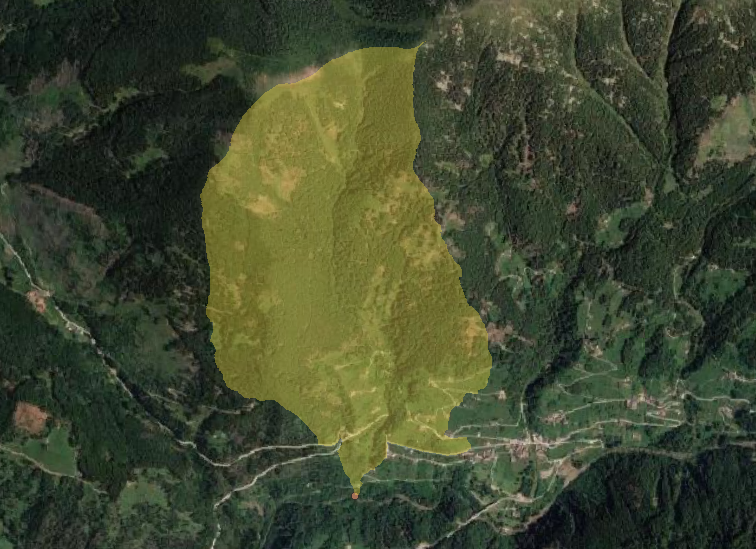
\includegraphics[scale=.50]{immagini/bacino_qgis.PNG}
    \caption{Rappresentazione del bacino idrografico e della sua sezione di chiusura.}
    \label{bacino_qgis}
\end{figure}
\noindent Per migliorare la visione, e comprendere meglio il territorio in analisi, è possibile simulare il fenomeno di ombreggiamento creato dal sole sui versanti e sulle valli.
\begin{figure}[H]\centering
    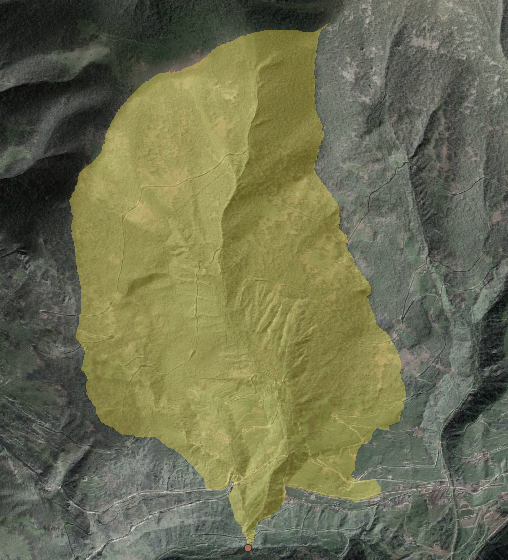
\includegraphics[scale=.50]{immagini/bacino_ombreggiatura_qgis.PNG}
    \caption{Rappresentazione del bacino idrografico, della sua sezione di chiusura e dell'effetto di ombreggiamento.}
    \label{bacino_ombreggiatura_qgis}
\end{figure}

\begin{figure}[H]
    \centering
    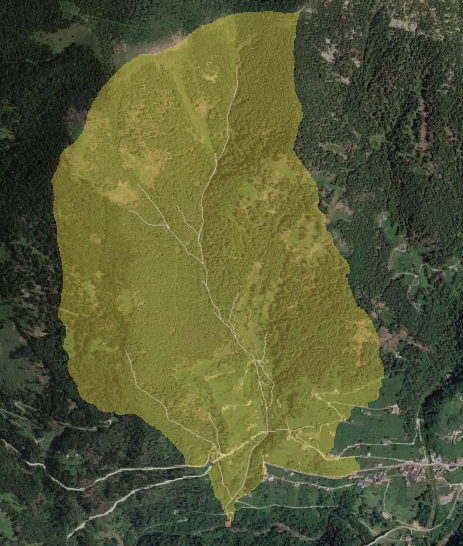
\includegraphics[scale=0.60]{immagini/bacino_reticolo_ombreg_qgis.PNG}
    \caption{Rappresentazione del bacino e del reticolo idrografico, con indicazione della sezione di chiusura.}
    \label{bacino_reticolo_qgis}
    \end{figure}

\noindent Dal reticolo idrografico di un bacino è possibile svolgere alcune considerazioni, come per esempio quella riguardante i suoi segmenti.\\
A seconda del numero di segmenti di cui è formato il reticolo, il bacino assume lo stesso valore di ordine, detto ``ordine del bacino" ed indicato con la lettera $k$.\\
Secondo il metodo di Horton-Strahler, l'attribuzione dell'ordine al segmento del reticolo idrografico avviene mediante tre regole: 
\begin{enumerate}
    \item ai tratti iniziali (di sorgente) viene attribuito valore 1;
    \item nel caso di confluenza di due tratti di diverso ordine, al segmento a valle viene attribuito il valore maggiore tra i due;
    \item nel caso di confluenza di due tratti con ordine $x$, al segmento a valle viene attribuito un valore $x+1$.
\end{enumerate} 
Avendo assegnato ad ogni tratto un certo valore numerico, è possibile conoscere la numerosità di ogni ordine.
\begin{figure}[H]\centering
    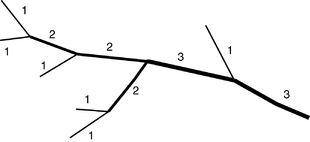
\includegraphics[scale=.75]{immagini/ordine_horton.png}
    \caption{Criterio di assegnazione dell'ordine ai segmenti del reticolo idrografico, secondo Horton-Strahler.}
  \label{ordine_horton}
\end{figure}
 
\paragraph{Reticolo idrografico secondo la CTP}
Nel caso di studio mediante l'utilizzo della Carta Tecnica Provinciale (\ref{scan_ctp}), il reticolo idrografico del bacino è formato da un'asta principale e da quattro tratti laterali, disposti sulla destra idraulica di quella maggiore.\\
Essendo che il segmento coincidente con il punto di chiusura possiede valore 3, di conseguenza l'intero bacino idrologico è di ordine 3.\\
La frequenza degli ordini dei segmenti è la seguente:
\begin{table}[H] \centering
    \begin{tabular}{cc}
\toprule
    Ordine u & Segmenti Nu \\
\midrule    
    1        & 5           \\
    2        & 2           \\
    3        & 1           \\
\bottomrule    
\end{tabular}
\end{table}
\paragraph{Reticolo idrografico secondo il DTM}
Studiando il reticolo idrografico generato dal DTM (\ref{bacino_reticolo_qgis}), si può osservare un maggiore numero di segmenti di ordine primo.\\
Anche in questo caso, l'ordine del bacino è di ordine 3.\\
La frequenza degli ordini dei segmenti è la seguente:
\begin{table}[H] \centering
    \begin{tabular}{cc}
\toprule
    Ordine u & Segmenti Nu \\
\midrule    
    1        & 12          \\
    2        & 3          \\
    3        & 1           \\
\bottomrule    
\end{tabular}
\end{table}

\subsection{Ulteriori caratteristiche del bacino}
\begin{figure}[H] 
    \begin{minipage}[]{7cm}
        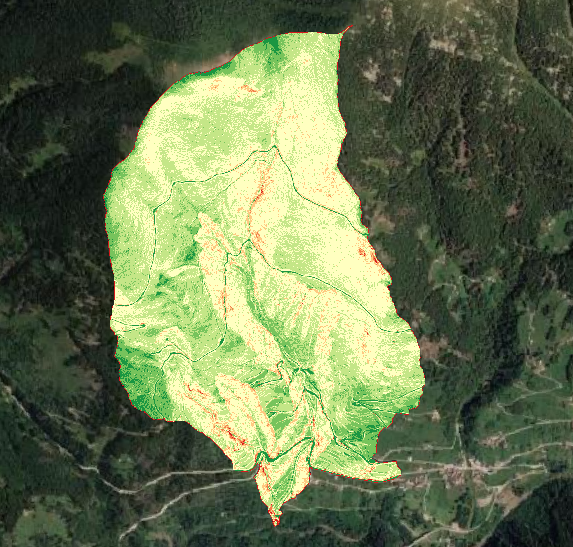
\includegraphics[scale=0.58]{immagini/bacino_slope.PNG}
        \caption{Rappresentazione della pendenza dei versanti del bacino.}
        \end{minipage}
        \hspace{2cm}
    \begin{minipage}[]{7cm}
        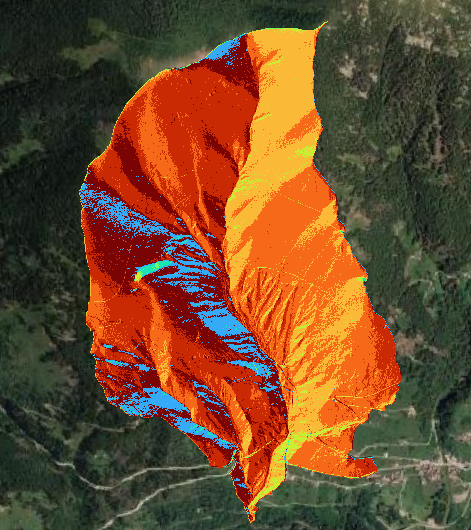
\includegraphics[scale=0.6]{immagini/bacino_orientamento_qgis.PNG}
        \caption{Orientamento dei versanti del bacino idrografico.}
    \end{minipage} 
        \end{figure}
       
\begin{figure}[H]  \centering
        \begin{minipage}[]{7cm}	
            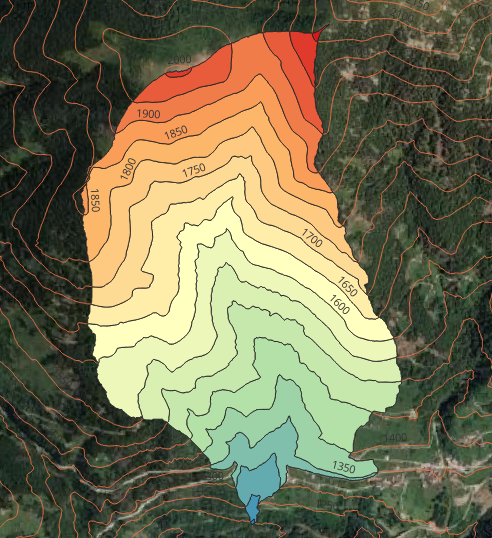
\includegraphics[scale=0.6]{immagini/bacino_fasce_quota_qgis.PNG}
        \caption{Rappresentazione delle fasce di quota altimetrica del bacino.}
        \end{minipage}  
\end{figure}

\section{Morfometria del bacino}
\subsection{Rapporto di biforcazione e prima legge di Horton}
Secondo la prima legge di Horton, il rapporto tra la numerosità dell'ordine precedente e la numerosità dell'ordine considerato (detto ``rapporto di biforcazione parziale")
\begin{equation}
    R_u = \frac{N_{u-1}}{N_u}
\end{equation}
è statisticamente costante, e regolata dalla funzione:
\begin{equation}
    N_u= \bar{R}_b ^{(k-u)}
\end{equation}
Dove: 
\begin{itemize}
    \item $R_b$ è la media tra i rapporti di biforcazione parziali;
    \item $k$ è l'ordine del bacino, nel caso di quello preso in considerazione il valore è 3;
    \item $u$ è l'ordine del tratto di reticolo considerato.
\end{itemize}
La prima legge di Horton inoltre, evidenzia come all'aumentare dell'ordine dei tratti, la lunghezza dei segmenti e le aree dei sottobacini aumentino, mentre cala la loro numerosità.\\
\paragraph{Reticolo idrografico, secondo la CTP} Nel caso del reticolo idrografico della CTP preso da noi in esame, i parametri sono: 

\begin{table}[H] \centering
    \caption{\textcolor{red}{Caratteristiche di biforcazione del reticolo idrografico ed applicazione della prima legge di Horton, secondo i dati ricavati dalla CTP.}}
    \label{tab:rapp_biforcazione_1_horton}
    \begin{tabular}{ cccc }
\toprule
    Ordine u & Segmenti Nu & Rapp. di biforcazione Rb & Nu (prima legge di Horton) \\
\midrule    
    1        & 5           &   /                     & 5.1                        \\
    2        & 2           & 2.5                      & 2.3                        \\
    3        & 1           & 2.0                      & 1.0                       \\
\bottomrule    
\end{tabular}
\end{table}
\noindent Il rapporto di biforcazione medio $\bar{R}_b$, secondo il ragionamento svolto sulla CTP è pari a \num{2.3}.\\
Interpolando i valori degli ordini dei segmenti, con la loro numerosità e con il parametro ricavato dalla prima legge di Horton, si ottiene un grafico caratteristico:
\begin{figure}[H]\centering
    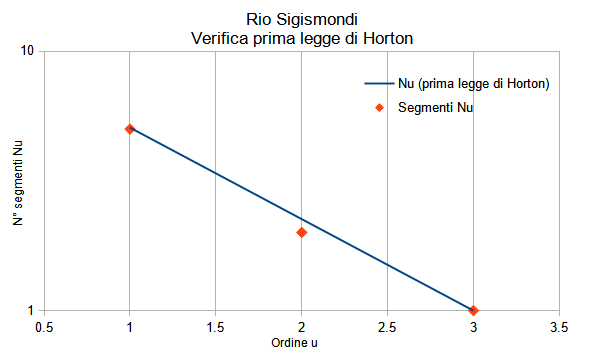
\includegraphics[scale=.75]{immagini/legge_horton.png}
    \caption{Relazione tra l'ordine del tratto, la sua numerosità e la funzione di Horton.}
    \label{legge_horton}
\end{figure}

\paragraph{Reticolo idrografico, secondo il DTM} Nel caso dello studio del reticolo idrografico mediante l'utilizzo di Qgis e del relativo file DTM, i parametri estratti sono i seguenti:
\begin{table}[H] \centering
    \caption{\textcolor{red}{Caratteristiche di biforcazione del reticolo idrografico ed applicazione della prima legge di Horton, secondo i dati ricavati dal DTM.}}
    \label{tab:rapp_biforcazione_2_horton}
    \begin{tabular}{ cccc }
\toprule
    Ordine u & Segmenti Nu & Rapp. di biforcazione Rb & Nu (prima legge di Horton) \\
\midrule    
    1        & 12          &   /        & 12.3                        \\
    2        & 3           & 4.0       & 3.5                        \\
    3        & 1           & 3.0      & 1.0                       \\
\bottomrule    
\end{tabular}
\end{table}

\noindent Il rapporto di biforcazione medio $\bar{R}_b$, secondo il ragionamento svolto sul DTM è pari a \num{3.5}.\\
Interpolando i valori degli ordini dei segmenti, con la loro numerosità e con il parametro ricavato dalla prima legge di Horton, si ottiene un grafico caratteristico:
\begin{figure}[H]\centering
    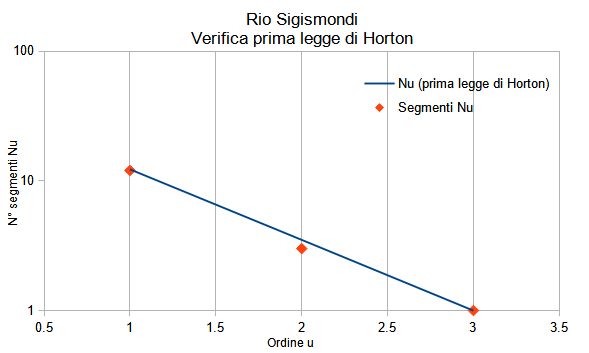
\includegraphics[scale=.75]{immagini/legge_horton_qgis.png}
    \caption{Relazione tra l'ordine del tratto, la sua numerosità e la funzione di Horton.}
    \label{legge_horton_qgis}
\end{figure}

\vspace{1cm}
In entrambi i casi, la prima legge di Horton viene soddisfatta, poichè la funzione del grafico interpola correttamente i dati reali del reticolo idrografico.\\
Lo scostamento dei dati nei due casi è dovuto alla differente estrazione del reticolo idrografico nei due metodi.

\subsection{Coefficiente di forma di Gravelius}
Il coefficiente di forma di Gravelius è un parametro che indica quanto la forma di un bacino sia compatta.\\
Questo indicatore confronta le misure di area e perimetro del bacino in analisi, con le misure che avrebbe un cerchio di uguale superficie; quindi, più l'indice tende ad uno e maggiore sarà la compattezza dell'area studiata.\\
Al fine di applicare la relativa formula, è necessario conoscere i valori di perimetro del bacino (lunghezza dello spartiacque), e l'area della superficie dell'intera area di studio.\\
La formula dell'indicatore è:
\begin{equation}
    F = \frac{0.28 \cdot P}{\sqrt{A}} = \frac{0.28 \cdot 8.690}{2.01} = 1.21
    \label{gravelius}
\end{equation}

\subsection{Indice di compattezza $F_c$}
Proprio come per l'indice precedente, questa formula permette di comprendere la forma del bacino.\\
Al contrario del coefficiente precedente, che utilizza il valore del perimetro, questa formula necessita di conoscere la lunghezza del reticolo idrografico del bacino, oltre che alla superficie drenante interna allo spartiacque.\\
La formula dell'indicatore è:
\begin{equation}
    F_c = \frac{L}{\sqrt{A}} = \frac{5.290}{\sqrt{2.01}} = 1.42
    \label{compatezza}
\end{equation}

\subsection{Indice di Melton}
L'indice di Melton quantifica l'energia potenziale (gravitativa) del bacino.\\
La formula è applicabile conoscendo il dislivello di quota tra quella massima del bacino e quella dell'apice del cono di deiezione, oltre che l'area totale del bacino. 
\begin{equation}
    Me = \frac{\Delta H}{\sqrt{A}}
    \label{melton}
\end{equation}
Questo fattore è importate per valutare i processi di trasporto solido che potrebbero avvenire; infatti, se questo valore è maggiore (o uguale) a 0.5, l'energia potenziale dei sedimenti potrebbe da dare luogo a fenomeni di trasporto, come per esempio le colate detritiche.

\subsection{Densità di drenaggio}
Questo indicatore, anche detto \textit{``drainage density"}, mette in relazione la lunghezza complessiva di tutti i rami del reticolo idrografico e l'area del bacino.\\
Tale valore è molto influenzato dalla quantità pluviometrica annua, dalle caratteristiche del suolo (litologia ed erodibilità) e dalla destinazione d'uso dell'area (copertura vegetale, impermeabilizzazione antropica,\dots).\\
La formula è:
\begin{equation}
    D_r = \frac{\Sigma L_i}{A} = \frac{5.290}{2.01} = 2.63 km^{-1}
    \label{drenaggio}
\end{equation}

\subsection{Indice di torrenzialità}
Questo indice rapporta il numero dei rami del reticolo con l'area totale del bacino idrografico.
La formula è:
\begin{equation}
I_t = \frac{N}{A} = \frac{16}{2.01} = 7.96 \hspace{3pt}\frac{n. segmenti}{km^2} 
\label{torrenzialità}
\end{equation}

\subsection{Quota media del bacino}
Questo valore quantifica l'altezza media del bacino rispetto alla sezione di chiusura, ponderando l'area.\\
Dal punto di vista geometrico, la quota media del bacino è il valore che, se introdotto nell'asse delle ordinate, crea un rettangolo di area uguale a quella sottesa alla curva ipsografica, aventi entrambi gli stessi valori in ascissa.\\
La formula è:
\begin{equation}
    H_m = h_m - h_0 = \frac{\Sigma (\bar{h}_i - h_0) \cdot A_i}{A}
    \label{quota_media}
\end{equation}

\noindent I calcoli, svolti in un foglio di calcolo elettronico, sono qui sotto riportati.

\begin{table}[H]
    \begin{tabular}{cccccccc}
        \toprule
    Quote (m s.l.m.) & n° celle & $A_i$ ($m^2$) & $A_i$ ($km^2$) & $Hi_{min}$ & $Hi_{max}$ & $Hi_{media}$ & $A_i \cdot Hi_{media}$ \\
   \midrule
    1183-1200                 & 261      & 261     & 0.000261 & 1183   & 1200   & 1192     & 0.311         \\
    1200-1250                 & 4874     & 4874    & 0.004874 & 1200   & 1250   & 1225     & 5.971         \\
    1250-1300                 & 27605    & 27605   & 0.027605 & 1250   & 1300   & 1275     & 35.196        \\
    1300-1350                 & 57101    & 57101   & 0.057101 & 1300   & 1350   & 1325     & 75.659        \\
    1350-1400                 & 108630   & 108630  & 0.10863  & 1350   & 1400   & 1375     & 149.366       \\
    1400-1450                 & 138207   & 138207  & 0.138207 & 1400   & 1450   & 1425     & 196.944       \\
    1450-1500                 & 160541   & 160541  & 0.160541 & 1450   & 1500   & 1475     & 236.797       \\
    1500-1550                 & 164185   & 164185  & 0.164185 & 1500   & 1550   & 1525     & 250.381       \\
    1550-1600                 & 199048   & 199048  & 0.199048 & 1550   & 1600   & 1575     & 313.500       \\
    1600-1650                 & 178951   & 178951  & 0.178951 & 1600   & 1650   & 1625     & 290.794       \\
    1650-1700                 & 175437   & 175437  & 0.175437 & 1650   & 1700   & 1675     & 293.856       \\
    1700-1750                 & 158025   & 158025  & 0.158025 & 1700   & 1750   & 1725     & 272.592       \\
    1750-1800                 & 152704   & 152704  & 0.152704 & 1750   & 1800   & 1775     & 271.049       \\
    1800-1850                 & 150620   & 150620  & 0.15062  & 1800   & 1850   & 1825     & 274.881       \\
    1850-1900                 & 115773   & 115773  & 0.115773 & 1850   & 1900   & 1875     & 217.074       \\
    1900-1950                 & 114122   & 114122  & 0.114122 & 1900   & 1950   & 1925     & 219.684       \\
    1950-2000                 & 82232    & 82232   & 0.082232 & 1950   & 2000   & 1975     & 162.408       \\
    2000-2050                 & 18149    & 18149   & 0.018149 & 2000   & 2050   & 2025     & 36.752        \\
    2050-2085                 & 1317     & 1317    & 0.001317 & 2050   & 2085   & 2067     & 2.723        \\
    \bottomrule
\end{tabular}
    \end{table}
\noindent Dove:
\begin{itemize}
    \item Quote: fasce di quota, secondo le linee di livello ortometriche;
    \item n° celle: numero di celle del raster, contenute in ogni fascia di quota;
    \item $A_i$: area di territorio ricadente in ogni fascia di quota (sia in $m^2$ che in $km^2$);
    \item $Hi_{min}$ e $Hi_{max}$: quota minima e massima della fascia di quota;
    \item $Hi_{media}$: valore altimetrico medio per ogni fascia di quota;
    \item $A_i \cdot Hi_{media}$: altezza media di ogni fascia altimetrica, soppesata per la propria estensione.
\end{itemize}
Considerando che le celle hanno estensione 1 $m^2$, l'area di ogni fascia di quota equivale (in $m^2$) al proprio numero di quadrati della matrice.\\
Essendo che l'area totale del bacino è di 2.01 $km^2$, la formula \ref{quota_media}, ricavata dal foglio di calcolo elettronico, restituisce il valore di 1646 $m$ sul livello del mare.

\subsection{Curva ipsometrica del bacino}
Al fine di valutare la condizione di dinamica temporale del bacino, risulta utile valutare le curve ipsometriche dello stesso.\\
Osservando l'andamento della curva che lega l'area del bacino e la quota ortometrica (siano queste dimensionali o adimensionali), è possibile capire se l'ara studiata è in una condizione giovanile (dove prevale l'erosione), maturità (equilibrio) o senilità.
\begin{figure}[H] \centering
          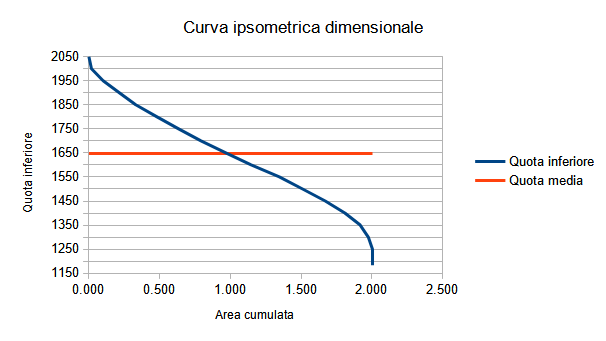
\includegraphics[scale=0.7]{immagini/curva_ipsografica_dimens.png}
        \caption{Curva ipsografica dimensionale del bacino. In ascissa è indicato il valore di area cumulata, ed in ordinata la relativa quota ortometrica.}
\end{figure}    
\begin{figure}[H] \centering
        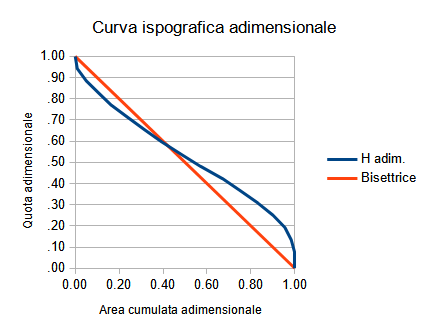
\includegraphics[scale=0.8]{immagini/curva_ipsografica_adimens.png}
        \caption{Curva ipsografica adimensionale del bacino. Al contrario dell'altro grafico, i valori degli assi sono adimensionali, ovvero rapportati con i massimi della serie.}
\end{figure}
Mediante entrambi i grafici è possibile osservare come il bacino si trovi in uno stato di equilibrio.\\
Mediante la bisettrice, nel secondo grafico, si può apprezzare maggiormente come, verso monte del bacino, l'erosione sia stata maggiore rispetto che a valle.

\subsection{Pendenza media dei versanti del bacino $i_m$}
L'indicatore in questione evidenzia, in modo mediato, la pendenza dei versanti del bacino.\\
Per calcolare tale numero si utilizza il Metodo Harlvord-Horton, mediante la formula:
\begin{equation}
    i_m = \Delta h \cdot \frac{\Sigma l_i}{A}
\end{equation}
dove: 
\begin{itemize}
 \item $l_i$ è la lunghezza totale dell'isoipsa considerata e delimitata all'interno dell'area del bacino;
 \item $A$ è la superficie totale del bacino idrografico.
\end{itemize}

\subsection{Caratteristiche del bacino idrografico}
Successivamente ad aver analizzato in modo completo il bacino idrografico, è possibile redigere una tabella riassuntiva.
\begin{table}[H] \centering
    \caption{\textcolor{red}{Caratteristiche del bacino idrografico  del torrente Sigismondi chiuso a ...}}
    \label{tab:caratteristiche_bacino}
    \begin{tabular}{ cccc } 
    \toprule
    Superficie planimetrica & A &  $\left[km^2\right]$ & 2.01 \\ 
    Perimetro & P & $\left[m\right]$        &      8690       \\ 
    Quota massima & $h_{max}$&  $\left[m s.m.\right]$       &    2084.6     \\
    Quota della sezione di chiusura & $h_0$ & $\left[m s.m.\right]$        &       1186      \\ 
    Quota apice del conoide &$h_{ap}$& $\left[m s.m.\right]$ & \\ 
    Quota media& $H_m$ & $\left[m s.m.\right]$ & 1646    \\ 
    Rilievo del bacino:& $h_{max} - h_o$ & $\left[m\right]$ &   901 \\ 
    Lunghezza del reticolo idrografico& $L_r$& $\left[m\right]$ & 5294,1 \\ 
    Pendenza media del bacino& $i_m$ & $\left[\%\right]$ & 54.19    \\ 
    Pendenza media del bacino& $i_m$& $\left[ ^\circ \right]$ & 28.45   \\ 
    Coefficiente di forma di Gravelius& F& $\left[\frac{0.28 \cdot P}{A^{0.5}} \right]$ & 1.21\\  
    Indice di compattezza &$F_c$  & $ \left[\frac{L}{A^{0.5}}\right]$ & 1.42\\ 
    Numero di Melton& & $\left[-\right]$ & \\ 
    Densità di drenaggio &$D_r$& $\left[\si{\km^{-1}}\right]$& 2.63 \\ 
    $N_1$& & & 12 \\ 
    Indice di torrenzialità& &$\left[\frac{n. segmenti }{km^2}\right]$ & 7.96 \\  
    Ordine di bacino& $k$ & $\left[-\right]$ & 3 \\ 
    Rapporto di biforcazione medio& $R_b$ & $\left[-\right]$ &  3.5 \\  
    Pendenza media del collettore principale & & $\left[\frac{m}{m}\right]$ & \\  
    \bottomrule
\end{tabular}
\end{table}
\section{Elaborazione statistico-probabilistica delle pioggie intense della stazione di riferimento per il bacino in esame (analisi degli afflussi)}
In questo capitolo della relazione si condurrà un'analisi statistico-probabilistica degli eventi pluviometrici del bacino. In particolare, si utilizzerà la distribuzione di probabilità dei valori estremi (legge di Gumbel).\\
Successivamente, verrà effettuata la verifica dell'adattamento della serie di valori pluviometrici alla distribuzione, facendo ricorso al test di Matalas.\\
Infine, si svolgeranno i calcoli per determinare la Linea Segnalatrice di Possibilità Pluviometrica (LSPP).\\
Essendo che si andrà a svolgere i calcoli considerando solamente i massimi annuali di precipitazione, occorre che tali valori debbano: 
\begin{itemize}
    \item essere relativi ad un certo periodo di tempo (almeno 30 anni);
    \item essere \textit{casuali, omogenei, indipendenti e stazionari}.
\end{itemize} 
In particolare, essendo la procedura di calcolo uguale per ogni serie numerica, verrà svolta la spiegazione per la durata pluviometrica di 30 minuti, per poi riportare solamente i risultati.

\subsection{Verifica preliminare visiva  (mediante \textit{Plotting position} e distribuzione delle classi)}
\label{sec_plotting_position}
Prima di svolgere l'adattamento della serie pluviometrica misurata a quella degli estremi di Gumbel, occorre valutare se tali valori si adattano correttamente lungo la retta di distribuzione teorica.\\
Ad ogni misura della serie, posta in ordine crescente, viene attribuito un valore a seconda della propria posizione nel campione, secondo il metodo di Weibull $(P_{em}= \frac{i}{N+1})$ o Hazen $\left(P_{em}=\frac{i-0.5}{N}\right)$. Entrambi questi parametri correlano l'evento di precipitazione con la probabilità di non superamento dell'evento (anche indicato come $P$).\\
Utilizzando il valore ricavato da uno di questi metodi, viene calcolata una variabile d'appoggio ($y$), secondo la formula $y = -ln(-ln(P))$, essendo che $P(x)= e ^{-e^ {-y}}$.\\
Successivamente, utilizzando i parametri $y$ (appena calcolato), $\alpha$ e $u$, quest'ultimi basati sul campione, si riesce a ricavare l'altezza di precipitazione dell'evento, regolarizzata secondo la distribuzione di Gumbel, secondo la formula inversa di $y = \alpha (h - u)$.
\begin{equation}
    \alpha = \left(\frac{1.283}{\sigma(h)}\right)
\end{equation}
\begin{equation}
    u = \left( h_m - \frac{0.5772}{\alpha} \right)
\end{equation}
\begin{equation}
    h = \frac{y}{\alpha}+u
    \label{h_tr}
\end{equation}
Al fine di verificare visivamente la bontà degli allineamenti delle distribuzioni della serie osservata e della serie attesa (teorica), occorre creare un grafico dove, in ascissa si pone il valore del parametro $y$ ed in ordinata si pongono i valori delle relative precipitazioni teoriche. I grafici sono riportati nel successivo capitoletto.\\
Maggiore è l'allineamento tra le due distribuzioni e migliore sarà la distribuzione della serie osservata.\\
Inoltre, per valutare preliminarmente la serie, può essere utile suddividere le precipitazioni per classi omogenee (per vedere come si distribuiscono i valori all'interno di esse) e calcolare i principali parametri statistici.

\begin{table}[H] \centering
    \caption{\textcolor{red}{Valori di probabilità di non superamento dell'evento (calcolata mediante Weibull e Hazen) e relativo valore del parametro d'appoggio $y$, riferito ad una durata di precipitazione di 0.5 ore.}}
    \begin{tabular}{cccccc}
 &  & \multicolumn{2}{c}{\textbf{Plotting Position}} & \multicolumn{2}{c}{\textbf{Y -ln( -ln (1- 1/Tr))}}\\
 \toprule
    \textbf{n} & \textbf{h [mm] 0.5 ore} & \textbf{P Weibull   n/N+1} & \textbf{P Hazen  (n-0,5)/N} & \textbf{y Weibull} & \textbf{y Hazen}\\
\midrule
    1          & 11.2                        & 0.026                      & 0.014                       & -1.291                  & -1.460                  \\
    2          & 12                          & 0.053                      & 0.041                       & -1.080                  & -1.165                  \\
    3          & 12.2                        & 0.079                      & 0.068                       & -0.932                  & -0.991                  \\
    4          & 12.6                        & 0.105                      & 0.095                       & -0.812                  & -0.858                  \\
    5          & 13.8                        & 0.132                      & 0.122                       & -0.707                  & -0.745                  \\
    6          & 14.2                        & 0.158                      & 0.149                       & -0.613                  & -0.645                  \\
    7          & 15                          & 0.184                      & 0.176                       & -0.526                  & -0.553                  \\
    8          & 16                          & 0.211                      & 0.203                       & -0.443                  & -0.468                  \\
    9          & 16.4                        & 0.237                      & 0.230                       & -0.365                  & -0.386                  \\
    10         & 16.6                        & 0.263                      & 0.257                       & -0.289                  & -0.307                  \\
    11         & 17.2                        & 0.289                      & 0.284                       & -0.215                  & -0.231                  \\
    12         & 17.4                        & 0.316                      & 0.311                       & -0.142                  & -0.156                  \\
    13         & 17.4                        & 0.342                      & 0.338                       & -0.070                  & -0.082                  \\
    14         & 18                          & 0.368                      & 0.365                       & 0.001                   & -0.008                  \\
    15         & 18                          & 0.395                      & 0.392                       & 0.073                   & 0.065                   \\
    16         & 18.6                        & 0.421                      & 0.419                       & 0.145                   & 0.139                   \\
    17         & 19                          & 0.447                      & 0.446                       & 0.218                   & 0.214                   \\
    18         & 19.6                        & 0.474                      & 0.473                       & 0.291                   & 0.289                   \\
    19         & 20                          & 0.500                      & 0.500                       & 0.367                   & 0.367                   \\
    20         & 20.2                        & 0.526                      & 0.527                       & 0.443                   & 0.446                   \\
    21         & 20.4                        & 0.553                      & 0.554                       & 0.522                   & 0.527                   \\
    22         & 21                          & 0.579                      & 0.581                       & 0.604                   & 0.611                   \\
    23         & 22.4                        & 0.605                      & 0.608                       & 0.689                   & 0.698                   \\
    24         & 22.6                        & 0.632                      & 0.635                       & 0.778                   & 0.790                   \\
    25         & 22.6                        & 0.658                      & 0.662                       & 0.871                   & 0.886                   \\
    26         & 23.4                        & 0.684                      & 0.689                       & 0.969                   & 0.988                   \\
    27         & 25.6                        & 0.711                      & 0.716                       & 1.074                   & 1.097                   \\
    28         & 25.6                        & 0.737                      & 0.743                       & 1.186                   & 1.215                   \\
    29         & 25.8                        & 0.763                      & 0.770                       & 1.308                   & 1.343                   \\
    30         & 26.6                        & 0.789                      & 0.797                       & 1.442                   & 1.485                   \\
    31         & 27                          & 0.816                      & 0.824                       & 1.592                   & 1.644                   \\
    32         & 27                          & 0.842                      & 0.851                       & 1.761                   & 1.827                   \\
    33         & 27.8                        & 0.868                      & 0.878                       & 1.958                   & 2.043                   \\
    34         & 27.8                        & 0.895                      & 0.905                       & 2.196                   & 2.309                   \\
    35         & 29.4                        & 0.921                      & 0.932                       & 2.498                   & 2.660                   \\
    36         & 32.6                        & 0.947                      & 0.959                       & 2.918                   & 3.185                   \\
    37         & 38.4                        & 0.974                      & 0.986                       & 3.624                   & 4.297         \\
    \bottomrule         
    \end{tabular}
    \end{table}

\begin{table}[H] \centering
    \caption{\textcolor{red}{Principali parametri statistici riferiti alla serie pluviometrica di durata 0.5 ore.}}
 \begin{tabular}{cc}
    \toprule
deviazione standard ($\sigma$) & 6.2  \\
media ($x_m$)              & 20.8 \\
$\alpha$            & 0.2  \\
$u$           & 18.1\\
N                & 37.0 \\
minimo ($x_{min}$)             & 11.2 \\
massimo ($x_{max}$)            & 38.4 \\
varianza ($\sigma^2$)             & 38.3 \\
coeff. variazione (CV)    & 0.30 \\
mediana ($x_{mediana}$)        & 20.0 \\
numero di classi (k)      & 5.5  \\
k scelto                 & 6.0  \\
verifica (Iman e Conover) & 64.0 \\
delta classe ($\Delta$)          & 4.5  \\
delta scelto             & 5.0 \\
        \bottomrule
        \end{tabular}
\end{table}    

La varianza ($\sigma ^2$) è un fattore che indica come i valori della serie si discostano dal quello medio (o da uno atteso).\\
La deviazione standard ($\sigma$), in modo simile alla variazione, indica la dispersione della serie numerica rispetto alla media; al contrario dell'indice statistico precedente, questo valore ha la stessa unità di misura della serie numerica, permettendo quindi il reciproco confronto.\\
Anche il coefficiente di variazione permette il confronto di fenomeni fisici o statistici aventi unità di misura differenti, essendo un parametro adimensionale.\\
La verifica di Iman e Conover ($2^k>N$) permette valutare se il numero di classi scelto per suddividere la serie è sufficientemente alto, per non averne un numero troppo basso e con un'alta densità di valori.\\
Il delta della classe ($\Delta$) indica la differenza tra il massimo valore della classe ed il minimo.

\begin{figure}[H]\centering
    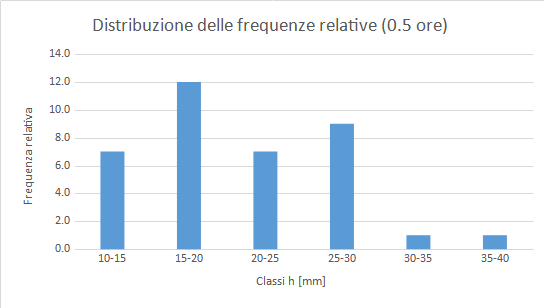
\includegraphics[scale=.6]{immagini/freq_piogg_rel_05ore.png}
    \caption{Distribuzione delle frequenze relative di pioggia (suddivise per classi omogenee), di un evento di durata 0.5 ore.}
  \label{freq_rel_piogg_05ore}
\end{figure}

\begin{figure}[H]\centering
    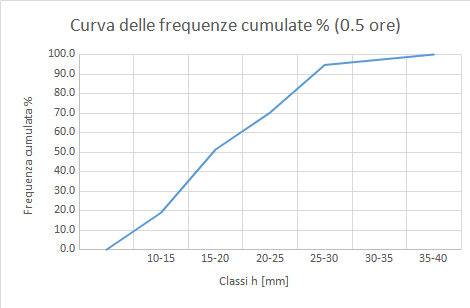
\includegraphics[scale=.6]{immagini/freq_piogg_cum_05ore.png}
    \caption{Frequenze di pioggia cumulata, relative ad un evento di durata 0.5 ore.}
  \label{freq_cum_piogg_05ore}
\end{figure}

\subsection{Calcolo delle altezze di pioggia per il $T_r$ di riferimento}
Successivamente ad aver verificato che l'allineamento tra le due distribuzioni è apprezzabile, occorre svolgere il calcolo delle altezze di pioggia, dati dei tempi di ritorno.\\
Essendo che $y = -ln(-ln(P))$ e $P = 1-\frac{1}{T_r}$, allora 
\begin{equation}
y = -ln\left(-ln\left(1-\frac{1}{T_r}\right)\right)
\end{equation}
Partendo da questo calcolo della variabile d'appoggio, è possibile ricavare l'altezza di precipitazione mediante la formula \ref{h_tr}.

\begin{table}[H] \centering
    \caption{\textcolor{red}{Valori di altezza di pioggia attesa (teorica), calcolata mediante la variabile d'appoggio $y$ di Weibull o di Hazen.}}
    \begin{tabular}{cccc}
 & & \multicolumn{2}{c}{$h = Y/\alpha + u$}       \\
 \toprule
    \textbf{n} & \textbf{h (mm)     0.5 ore} & \textbf{h mediante Weibull} & \textbf{h mediante Hazen} \\
\midrule
    1          & 11.2                        & 11.839                & 11.028                 \\
    2          & 12                          & 12.858                & 12.449                 \\
    3          & 12.2                        & 13.573                & 13.286                 \\
    4          & 12.6                        & 14.153                & 13.929                 \\
    5          & 13.8                        & 14.656                & 14.472                 \\
    6          & 14.2                        & 15.110                & 14.955                 \\
    7          & 15                          & 15.531                & 15.397                 \\
    8          & 16                          & 15.927                & 15.811                 \\
    9          & 16.4                        & 16.306                & 16.205                 \\
    10         & 16.6                        & 16.672                & 16.584                 \\
    11         & 17.2                        & 17.029                & 16.953                 \\
    12         & 17.4                        & 17.380                & 17.314                 \\
    13         & 17.4                        & 17.727                & 17.671                 \\
    14         & 18                          & 18.073                & 18.026                 \\
    15         & 18                          & 18.418                & 18.380                 \\
    16         & 18.6                        & 18.765                & 18.737                 \\
    17         & 19                          & 19.115                & 19.096                 \\
    18         & 19.6                        & 19.471                & 19.461                 \\
    19         & 20                          & 19.833                & 19.833                 \\
    20         & 20.2                        & 20.203                & 20.214                 \\
    21         & 20.4                        & 20.585                & 20.606                 \\
    22         & 21                          & 20.979                & 21.011                 \\
    23         & 22.4                        & 21.388                & 21.433                 \\
    24         & 22.6                        & 21.815                & 21.874                 \\
    25         & 22.6                        & 22.263                & 22.338                 \\
    26         & 23.4                        & 22.738                & 22.831                 \\
    27         & 25.6                        & 23.243                & 23.356                 \\
    28         & 25.6                        & 23.785                & 23.924                 \\
    29         & 25.8                        & 24.374                & 24.542                 \\
    30         & 26.6                        & 25.020                & 25.225                 \\
    31         & 27                          & 25.740                & 25.993                 \\
    32         & 27                          & 26.557                & 26.874                 \\
    33         & 27.8                        & 27.509                & 27.915                 \\
    34         & 27.8                        & 28.655                & 29.199                 \\
    35         & 29.4                        & 30.111                & 30.891                 \\
    36         & 32.6                        & 32.133                & 33.422                 \\
    37         & 38.4                        & 35.541                & 38.786          \\
    \bottomrule      
    \end{tabular}
    \end{table}

    \begin{figure}[H]\centering
        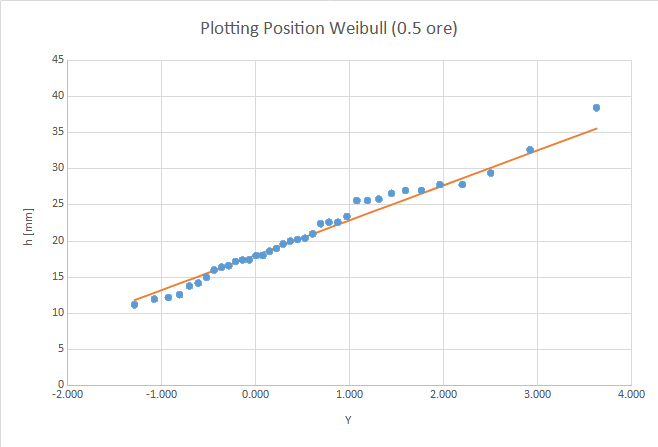
\includegraphics[scale=.5]{immagini/plot_pos_weib_05ore.png}
        \caption{Plotting position mediante weibull.}
      \label{plot_pos_weib_05ore}
    \end{figure}

    \begin{figure}[H]\centering
        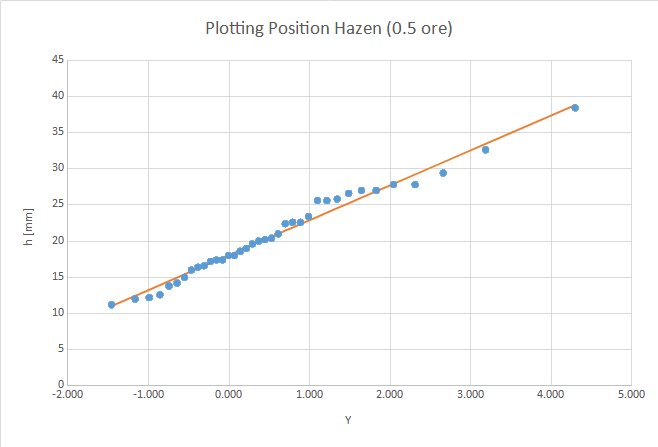
\includegraphics[scale=.5]{immagini/plot_pos_hazen_05ore.png}
        \caption{Plottin position mediante Hazen.}
      \label{plot_pos_hazen_05ore}
    \end{figure}

\begin{table}[H] \centering
    \caption{\textcolor{red}{Altezze di pioggia attese per il $T_r$ di riferimento e durata di 0.5 ore.}}
        \begin{tabular}{ccc}
        \toprule
        Tr (anni) & y     & h attesa (mm) \\
        \midrule
        2 & 0.367 & 19.8  \\
        5 & 1.500 & 25.3  \\
        10  & 2.250 & 28.9          \\
        30  & 3.384 & 34.4          \\
        50  & 3.902 & 36.9          \\
        100 & 4.600 & 40.2          \\
        200 & 5.296 & 43.6          \\         
        \bottomrule
        \end{tabular}
\end{table}
    
\subsection{Test statistico di Matalas}
Similmente a come è stata svolta la verifica grafica (\ref{sec_plotting_position}), è necessario accertarsi che l'asimmetria ($G$) della serie osservata (storica) non differisca eccessivamente dalla serie teorica.\\
La procedura del test statistico è:
\begin{itemize}
\item calcolo del coefficiente di asimmetria $G$, mediante \ref{coef_asimmetria};
\item estrapolazione dei parametri $E(y)$ e $\sigma(y)$, in funzione di N;
\item verifica della disequazione \ref{disequazione_matalas}.
\end{itemize}
\begin{equation}
    G = \frac{m_3}{m_2^{\frac{3}{2}}} = N^{\frac{1}{2}} \frac{\sum_{i=1,N}(x_i - x_m)^3}{\left[\sum_{i=1,N}(x_i-x_m)^2\right]^{\frac{3}{2}}}
    \label{coef_asimmetria}
\end{equation}
\begin{equation}
    |G - E (y)| < 2 \sigma(y)
    \label{disequazione_matalas}
\end{equation}
Dove:
\begin{itemize}
    \item $G$: coefficiente di asimmetria del campione;
    \item $E(y)$: coefficiente di asimmetria del campione perfetto, che segue l'andamento di Gumbel;
    \item $\sigma (y)$: deviazione standard del campione.
\end{itemize}
Nel caso in cui la disequazione fosse corretta, è possibile accettare la distribuzione di probabilità di Gumbel. In caso contrario occorrerebbe provare un'altra distribuzione teorica di probabilità.

\begin{table}[H] \centering
    \caption{\textcolor{red}{Parametri per l'esecuzione del test statistico di Matalas, relativi alla durata di precipitazione di 0.5 ore.}}
    \begin{tabular}{cc}
    \toprule
    media                  & 20.85 \\
    $N ^{0.5}$ & 6.083 \\
    G                      & 0.622 \\
    G - E                  & 0.259 \\
    2 $\sigma$             & 1.069 \\
    TEST                   & Vero \\
    \bottomrule
    \end{tabular}
\end{table}

\subsection{Risultati delle altre durate di precipitazione}
Come anticipato precedentemente, in questa sezione vengono riportati solamente i risultati delle analisi matematiche (tabelle e grafici) per le altre durate di precipitazione.\\
I procedimenti per le seguenti durate sono i medesimi utilizzati per la durata di 0.5 ore.
\subsubsection{Durata di 1 ora}
\begin{table}[H] \centering
    \caption{\textcolor{red}{Valori di probabilità di non superamento dell'evento (calcolata mediante Weibull e Hazen) e relativo valore del parametro d'appoggio $y$, riferito ad una durata di precipitazione di 1 ora.}}
    \begin{tabular}{cccccc}
        &  & \multicolumn{2}{c}{\textbf{Plotting Position}} & \multicolumn{2}{c}{\textbf{Y -ln( -ln (1- 1/Tr))}}\\
        \toprule
           \textbf{n} & \textbf{h [mm] 1 ora} & \textbf{P Weibull   n/N+1} & \textbf{P Hazen  (n-0,5)/N} & \textbf{y Weibull} & \textbf{y Hazen}\\
       \midrule
    1          & 13.8                      & 0.026                      & 0.014                       & -1.291                  & -1.460                  \\
    2          & 14.4                      & 0.053                      & 0.041                       & -1.080                  & -1.165                  \\
    3          & 16.2                      & 0.079                      & 0.068                       & -0.932                  & -0.991                  \\
    4          & 17                        & 0.105                      & 0.095                       & -0.812                  & -0.858                  \\
    5          & 17.6                      & 0.132                      & 0.122                       & -0.707                  & -0.745                  \\
    6          & 17.8                      & 0.158                      & 0.149                       & -0.613                  & -0.645                  \\
    7          & 19.2                      & 0.184                      & 0.176                       & -0.526                  & -0.553                  \\
    8          & 19.4                      & 0.211                      & 0.203                       & -0.443                  & -0.468                  \\
    9          & 19.4                      & 0.237                      & 0.230                       & -0.365                  & -0.386                  \\
    10         & 20.6                      & 0.263                      & 0.257                       & -0.289                  & -0.307                  \\
    11         & 20.6                      & 0.289                      & 0.284                       & -0.215                  & -0.231                  \\
    12         & 21.2                      & 0.316                      & 0.311                       & -0.142                  & -0.156                  \\
    13         & 21.6                      & 0.342                      & 0.338                       & -0.070                  & -0.082                  \\
    14         & 21.8                      & 0.368                      & 0.365                       & 0.001                   & -0.008                  \\
    15         & 23.6                      & 0.395                      & 0.392                       & 0.073                   & 0.065                   \\
    16         & 23.6                      & 0.421                      & 0.419                       & 0.145                   & 0.139                   \\
    17         & 23.8                      & 0.447                      & 0.446                       & 0.218                   & 0.214                   \\
    18         & 24                        & 0.474                      & 0.473                       & 0.291                   & 0.289                   \\
    19         & 24.2                      & 0.500                      & 0.500                       & 0.367                   & 0.367                   \\
    20         & 24.4                      & 0.526                      & 0.527                       & 0.443                   & 0.446                   \\
    21         & 24.4                      & 0.553                      & 0.554                       & 0.522                   & 0.527                   \\
    22         & 24.8                      & 0.579                      & 0.581                       & 0.604                   & 0.611                   \\
    23         & 25.8                      & 0.605                      & 0.608                       & 0.689                   & 0.698                   \\
    24         & 26.8                      & 0.632                      & 0.635                       & 0.778                   & 0.790                   \\
    25         & 27                        & 0.658                      & 0.662                       & 0.871                   & 0.886                   \\
    26         & 27.6                      & 0.684                      & 0.689                       & 0.969                   & 0.988                   \\
    27         & 28                        & 0.711                      & 0.716                       & 1.074                   & 1.097                   \\
    28         & 28.8                      & 0.737                      & 0.743                       & 1.186                   & 1.215                   \\
    29         & 30.2                      & 0.763                      & 0.770                       & 1.308                   & 1.343                   \\
    30         & 30.2                      & 0.789                      & 0.797                       & 1.442                   & 1.485                   \\
    31         & 30.4                      & 0.816                      & 0.824                       & 1.592                   & 1.644                   \\
    32         & 31.2                      & 0.842                      & 0.851                       & 1.761                   & 1.827                   \\
    33         & 31.6                      & 0.868                      & 0.878                       & 1.958                   & 2.043                   \\
    34         & 34.2                      & 0.895                      & 0.905                       & 2.196                   & 2.309                   \\
    35         & 37.8                      & 0.921                      & 0.932                       & 2.498                   & 2.660                   \\
    36         & 42.6                      & 0.947                      & 0.959                       & 2.918                   & 3.185                   \\
    37         & 49.8                      & 0.974                      & 0.986                       & 3.624                   & 4.297        \\
    \bottomrule          
    \end{tabular}
    \end{table}
    
\begin{table}[H] \centering
    \caption{\textcolor{red}{Principali parametri statistici riferiti alla serie pluviometrica di durata 1 ora.}}
        \begin{tabular}{cc}
    \toprule
        deviazione standard ($\sigma$)   & 7.5  \\
        media (xm)                & 25.3 \\
        $\alpha$                & 0.2  \\
        u                & 21.9 \\
        N                & 37.0 \\
        minimo ($x_{min}$)             & 13.8 \\
        massimo ($x_{max}$)            & 49.8 \\
        varianza ($\sigma ^2$)             & 56.6 \\
        coeff. Variazione (CV)    & 0.30 \\
        mediana ($x_{mediana}$)        & 24.2 \\
        numero di classi (k)      & 5.5  \\
        k scelto:                 & 6.0  \\
        verifica (Iman e Conover) & 64.0 \\
        delta classe ($\Delta$)          & 6.0  \\
        delta scelto             & 7.0 \\
        \bottomrule 
 \end{tabular}
\end{table}



\begin{figure}[H]\centering
    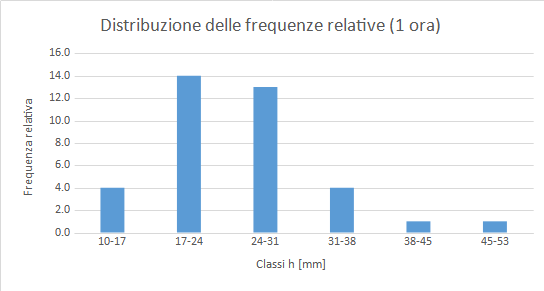
\includegraphics[scale=.6]{immagini/freq_piogg_rel_1ora.png}
    \caption{Distribuzione delle frequenze relative di pioggia (suddivise per classi omogenee), di un evento di durata 1 ora.}
  \label{freq_rel_piogg_05ore}
\end{figure}

\begin{figure}[H]\centering
    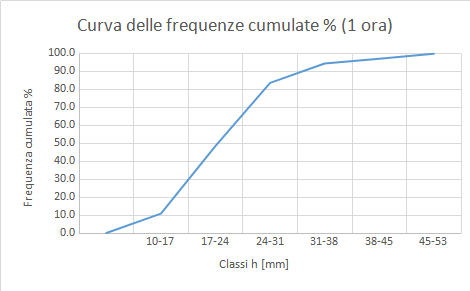
\includegraphics[scale=.6]{immagini/freq_piogg_cum_1ora.png}
    \caption{Frequenze di pioggia cumulata, relative ad un evento di durata 1 ora.}
  \label{freq_cum_piogg_05ore}
\end{figure}

\begin{table}[H] \centering
    \caption{\textcolor{red}{Valori di altezza di pioggia attesa (teorica), calcolata mediante la variabile d'appoggio $y$ di Weibull o di Hazen.}}
    \begin{tabular}{cccc}
 & & \multicolumn{2}{c}{$h = Y/\alpha + u$}       \\
 \toprule
    \textbf{n} & \textbf{h (mm)  1 ora} & \textbf{h mediante Weibull} & \textbf{h mediante Hazen} \\
\midrule
    n         & h (mm)     1 ora & h\_calc Weib   & h\_calc Hazen  \\
    1         & 13.8             & 14.322         & 13.335         \\
    2         & 14.4             & 15.562         & 15.063         \\
    3         & 16.2             & 16.431         & 16.082         \\
    4         & 17               & 17.136         & 16.864         \\
    5         & 17.6             & 17.748         & 17.525         \\
    6         & 17.8             & 18.301         & 18.112         \\
    7         & 19.2             & 18.812         & 18.650         \\
    8         & 19.4             & 19.294         & 19.154         \\
    9         & 19.4             & 19.755         & 19.633         \\
    10        & 20.6             & 20.201         & 20.094         \\
    11        & 20.6             & 20.635         & 20.542         \\
    12        & 21.2             & 21.062         & 20.982         \\
    13        & 21.6             & 21.484         & 21.416         \\
    14        & 21.8             & 21.904         & 21.848         \\
    15        & 23.6             & 22.324         & 22.279         \\
    16        & 23.6             & 22.746         & 22.712         \\
    17        & 23.8             & 23.172         & 23.149         \\
    18        & 24               & 23.605         & 23.593         \\
    19        & 24.2             & 24.045         & 24.045         \\
    20        & 24.4             & 24.496         & 24.509         \\
    21        & 24.4             & 24.960         & 24.985         \\
    22        & 24.8             & 25.439         & 25.479         \\
    23        & 25.8             & 25.937         & 25.992         \\
    24        & 26.8             & 26.456         & 26.528         \\
    25        & 27               & 27.002         & 27.093         \\
    26        & 27.6             & 27.579         & 27.692         \\
    27        & 28               & 28.193         & 28.332         \\
    28        & 28.8             & 28.853         & 29.022         \\
    29        & 30.2             & 29.569         & 29.774         \\
    30        & 30.2             & 30.355         & 30.605         \\
    31        & 30.4             & 31.231         & 31.539         \\
    32        & 31.2             & 32.225         & 32.610         \\
    33        & 31.6             & 33.382         & 33.877         \\
    34        & 34.2             & 34.777         & 35.438         \\
    35        & 37.8             & 36.548         & 37.496         \\
    36        & 42.6             & 39.008         & 40.576         \\
    37        & 49.8             & 43.153         & 47.100         \\
    \bottomrule
    \end{tabular}
    \end{table}

\begin{figure}[H]\centering
        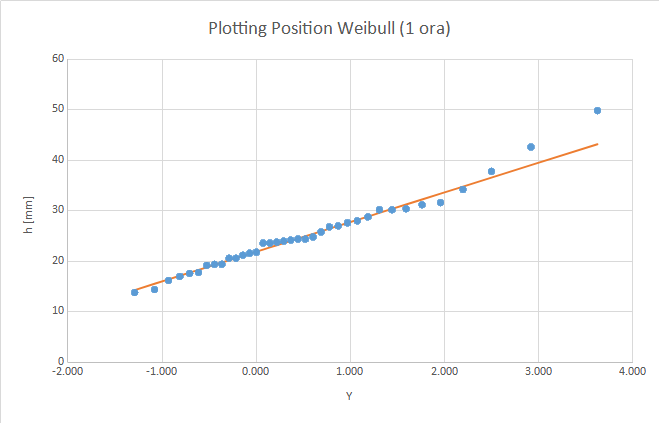
\includegraphics[scale=.5]{immagini/plot_pos_weib_1ora.png}
        \caption{Plotting position mediante Weibull.}
      \label{plot_pos_weib_1ora}
 \end{figure}

\begin{figure}[H]\centering
        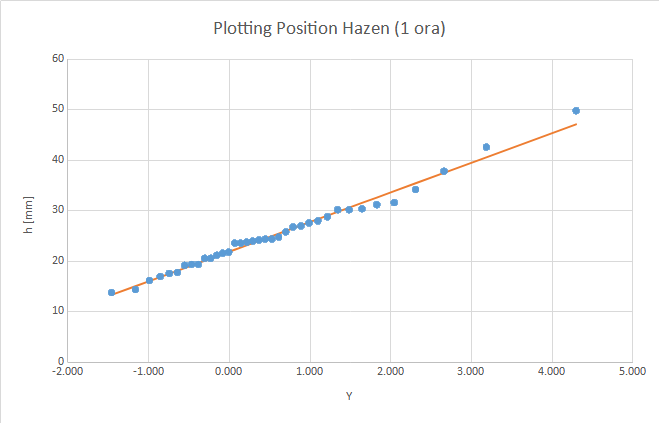
\includegraphics[scale=.5]{immagini/plot_pos_hazen_1ora.png}
        \caption{Plotting position mediante Hazen.}
      \label{plot_pos_hazen_1ora}
\end{figure}

\begin{table}[H] \centering
    \caption{\textcolor{red}{Altezze di pioggia attese per il $T_r$ di riferimento e durata di 1 ora.}}
        \begin{tabular}{ccc}
        \toprule
        Tr (anni) & y     & h attesa (mm) \\
        \midrule
        2 & 0.367 & 24.0  \\
        5 & 1.500 & 30.7  \\
        10  & 2.250 & 35.1          \\
        30  & 3.384 & 41.7          \\
        50  & 3.902 & 44.8          \\
        100 & 4.600 & 48.9          \\
        200 & 5.296 & 53.0          \\         
        \bottomrule
        \end{tabular}
\end{table}

\begin{table}[H] \centering
    \caption{\textcolor{red}{Parametri per l'esecuzione del test statistico di Matalas, relativi alla durata di precipitazione di 1 ora.}}
    \begin{tabular}{cc}
    \toprule
    media                  & 25.28 \\
    $N ^{0.5}$             &  6.083\\
    G                      & 1.158 \\
    G - E                  &  0.277\\
    2 $\sigma$             & 1.069 \\
    TEST                   & Vero \\
    \bottomrule
    \end{tabular}
\end{table}

\subsubsection{Durata di 3 ore}
\begin{table}[H] \centering
    \caption{\textcolor{red}{Valori di probabilità di non superamento dell'evento (calcolata mediante Weibull e Hazen) e relativo valore del parametro d'appoggio $y$, riferito ad una durata di precipitazione di 3 ore.}}
\begin{tabular}{cccccc}
    &  & \multicolumn{2}{c}{\textbf{Plotting Position}} & \multicolumn{2}{c}{\textbf{Y -ln( -ln (1- 1/Tr))}}\\
    \toprule
       \textbf{n} & \textbf{h [mm] 1 ora} & \textbf{P Weibull   n/N+1} & \textbf{P Hazen  (n-0,5)/N} & \textbf{y Weibull} & \textbf{y Hazen}\\
   \midrule 
    1          & 18.6                      & 0.026                      & 0.014                       & -1.291                  & -1.460                  \\
    2          & 19.6                      & 0.053                      & 0.041                       & -1.080                  & -1.165                  \\
    3          & 21.8                      & 0.079                      & 0.068                       & -0.932                  & -0.991                  \\
    4          & 21.8                      & 0.105                      & 0.095                       & -0.812                  & -0.858                  \\
    5          & 23.4                      & 0.132                      & 0.122                       & -0.707                  & -0.745                  \\
    6          & 24.6                      & 0.158                      & 0.149                       & -0.613                  & -0.645                  \\
    7          & 24.8                      & 0.184                      & 0.176                       & -0.526                  & -0.553                  \\
    8          & 25.4                      & 0.211                      & 0.203                       & -0.443                  & -0.468                  \\
    9          & 26.8                      & 0.237                      & 0.230                       & -0.365                  & -0.386                  \\
    10         & 27.8                      & 0.263                      & 0.257                       & -0.289                  & -0.307                  \\
    11         & 28                        & 0.289                      & 0.284                       & -0.215                  & -0.231                  \\
    12         & 30.4                      & 0.316                      & 0.311                       & -0.142                  & -0.156                  \\
    13         & 30.4                      & 0.342                      & 0.338                       & -0.070                  & -0.082                  \\
    14         & 31.2                      & 0.368                      & 0.365                       & 0.001                   & -0.008                  \\
    15         & 31.8                      & 0.395                      & 0.392                       & 0.073                   & 0.065                   \\
    16         & 32.8                      & 0.421                      & 0.419                       & 0.145                   & 0.139                   \\
    17         & 33                        & 0.447                      & 0.446                       & 0.218                   & 0.214                   \\
    18         & 33.2                      & 0.474                      & 0.473                       & 0.291                   & 0.289                   \\
    19         & 33.2                      & 0.500                      & 0.500                       & 0.367                   & 0.367                   \\
    20         & 33.8                      & 0.526                      & 0.527                       & 0.443                   & 0.446                   \\
    21         & 34                        & 0.553                      & 0.554                       & 0.522                   & 0.527                   \\
    22         & 35.4                      & 0.579                      & 0.581                       & 0.604                   & 0.611                   \\
    23         & 35.8                      & 0.605                      & 0.608                       & 0.689                   & 0.698                   \\
    24         & 35.8                      & 0.632                      & 0.635                       & 0.778                   & 0.790                   \\
    25         & 35.8                      & 0.658                      & 0.662                       & 0.871                   & 0.886                   \\
    26         & 36                        & 0.684                      & 0.689                       & 0.969                   & 0.988                   \\
    27         & 36.2                      & 0.711                      & 0.716                       & 1.074                   & 1.097                   \\
    28         & 37.2                      & 0.737                      & 0.743                       & 1.186                   & 1.215                   \\
    29         & 38.2                      & 0.763                      & 0.770                       & 1.308                   & 1.343                   \\
    30         & 38.4                      & 0.789                      & 0.797                       & 1.442                   & 1.485                   \\
    31         & 41.4                      & 0.816                      & 0.824                       & 1.592                   & 1.644                   \\
    32         & 41.6                      & 0.842                      & 0.851                       & 1.761                   & 1.827                   \\
    33         & 44.8                      & 0.868                      & 0.878                       & 1.958                   & 2.043                   \\
    34         & 45.8                      & 0.895                      & 0.905                       & 2.196                   & 2.309                   \\
    35         & 46                        & 0.921                      & 0.932                       & 2.498                   & 2.660                   \\
    36         & 50.6                      & 0.947                      & 0.959                       & 2.918                   & 3.185                   \\
    37         & 75.4                      & 0.974                      & 0.986                       & 3.624                   & 4.297              \\
    \bottomrule    
    \end{tabular}
    \end{table}

\begin{table}[H] \centering
        \caption{\textcolor{red}{Principali parametri statistici riferiti alla serie pluviometrica di durata 3 ore.}}
     \begin{tabular}{cc}
        \toprule
    deviazione standard ($\sigma$) & 10.3 \\
    media ($x_m$)              & 34.1 \\
    $\alpha$            &  0.1 \\
    $u$           & 29.4\\
    N                & 37 \\
    minimo ($x_{min}$)      & 18.6 \\
    massimo ($x_{max}$)     & 75.4 \\
    varianza ($\sigma^2$)            & 106.7 \\
    coeff. variazione (CV)    &  0.3\\
    mediana ($x_{mediana}$)        & 33.2 \\
    numero di classi (k)      & 5.5  \\
    k scelto                 &  6.0 \\
    verifica (Iman e Conover) & 64.0 \\
    delta classe ($\Delta$)          & 9.5  \\
    delta scelto             & 10.0 \\
            \bottomrule
            \end{tabular}
    \end{table}

\begin{figure}[H]\centering
        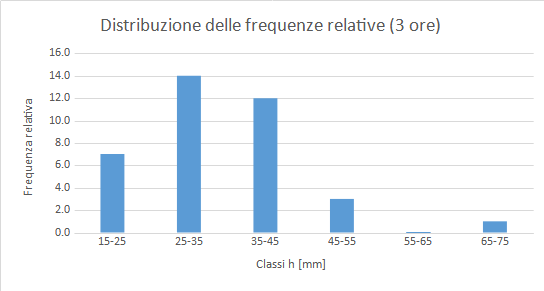
\includegraphics[scale=.6]{immagini/freq_piogg_rel_3ore.png}
        \caption{Distribuzione delle frequenze relative di pioggia (suddivise per classi omogenee), di un evento di durata 3 ore.}
      \label{freq_rel_piogg_05ore}
\end{figure}
    
\begin{figure}[H]\centering
        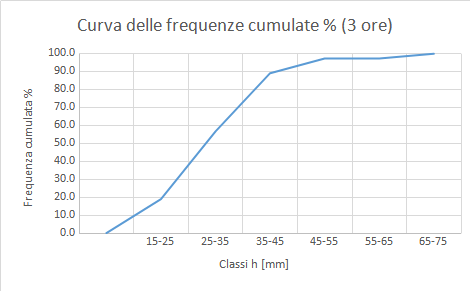
\includegraphics[scale=.6]{immagini/freq_piogg_cum_3ore.png}
        \caption{Frequenze di pioggia cumulata, relative ad un evento di durata 3 ore.}
      \label{freq_cum_piogg_05ore}
\end{figure}

\begin{table}[H] \centering
    \caption{\textcolor{red}{Valori di altezza di pioggia attesa (teorica), calcolata mediante la variabile d'appoggio $y$ di Weibull o di Hazen.}}
    \begin{tabular}{cccc}
 & & \multicolumn{2}{c}{$h = Y/\alpha + u$}       \\
 \toprule
    \textbf{n} & \textbf{h (mm)  3 ore} & \textbf{h mediante Weibull} & \textbf{h mediante Hazen} \\
\midrule
    1          & 18.6                      & 19.035                & 17.681                 \\
    2          & 19.6                      & 20.737                & 20.053                 \\
    3          & 21.8                      & 21.929                & 21.450                 \\
    4          & 21.8                      & 22.897                & 22.524                 \\
    5          & 23.4                      & 23.738                & 23.431                 \\
    6          & 24.6                      & 24.496                & 24.237                 \\
    7          & 24.8                      & 25.198                & 24.975                 \\
    8          & 25.4                      & 25.860                & 25.666                 \\
    9          & 26.8                      & 26.492                & 26.324                 \\
    10         & 27.8                      & 27.104                & 26.957                 \\
    11         & 28                        & 27.700                & 27.572                 \\
    12         & 30.4                      & 28.286                & 28.176                 \\
    13         & 30.4                      & 28.865                & 28.771                 \\
    14         & 31.2                      & 29.441                & 29.364                 \\
    15         & 31.8                      & 30.018                & 29.955                 \\
    16         & 32.8                      & 30.597                & 30.550                 \\
    17         & 33                        & 31.182                & 31.150                 \\
    18         & 33.2                      & 31.775                & 31.759                 \\
    19         & 33.2                      & 32.380                & 32.380                 \\
    20         & 33.8                      & 32.999                & 33.016                 \\
    21         & 34                        & 33.635                & 33.670                 \\
    22         & 35.4                      & 34.293                & 34.347                 \\
    23         & 35.8                      & 34.975                & 35.051                 \\
    24         & 35.8                      & 35.688                & 35.787                 \\
    25         & 35.8                      & 36.437                & 36.562                 \\
    26         & 36                        & 37.229                & 37.384                 \\
    27         & 36.2                      & 38.072                & 38.262                 \\
    28         & 37.2                      & 38.978                & 39.209                 \\
    29         & 38.2                      & 39.960                & 40.241                 \\
    30         & 38.4                      & 41.039                & 41.382                 \\
    31         & 41.4                      & 42.241                & 42.663                 \\
    32         & 41.6                      & 43.606                & 44.134                 \\
    33         & 44.8                      & 45.194                & 45.872                 \\
    34         & 45.8                      & 47.108                & 48.015                 \\
    35         & 46                        & 49.538                & 50.840                 \\
    36         & 50.6                      & 52.914                & 55.066                 \\
    37         & 75.4                      & 58.603                & 64.020          \\
    \bottomrule      
    \end{tabular}
    \end{table}

    \begin{figure}[H]\centering
        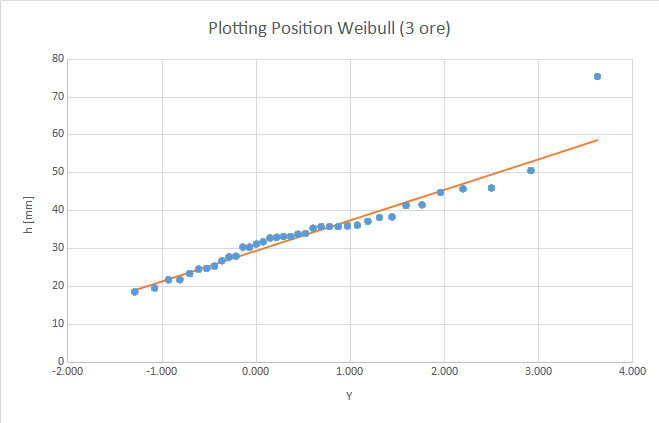
\includegraphics[scale=.5]{immagini/plot_pos_weib_3ore.png}
        \caption{Plotting position mediante Weibull.}
      \label{plot_pos_weib_3ore}
 \end{figure}

\begin{figure}[H]\centering
        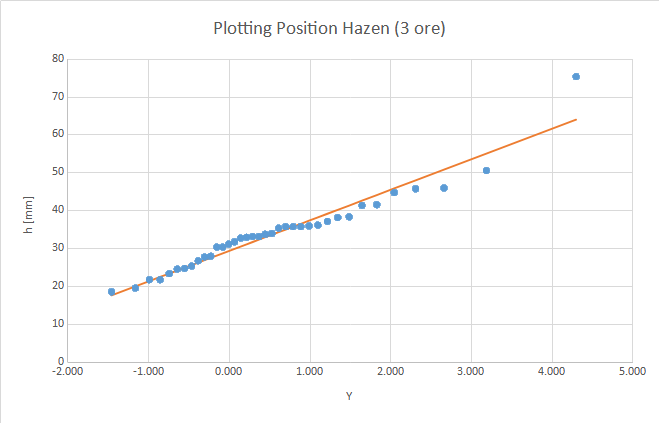
\includegraphics[scale=.5]{immagini/plot_pos_hazen_3ore.png}
        \caption{Plotting position mediante Hazen.}
      \label{plot_pos_hazen_3ore}
\end{figure}

\begin{table}[H] \centering
    \caption{\textcolor{red}{Altezze di pioggia attese per il $T_r$ di riferimento e durata di 3 ore.}}
        \begin{tabular}{ccc}
        \toprule
        Tr (anni) & y     & h attesa (mm) \\
        \midrule
        2 & 0.367 & 32.4  \\
        5 & 1.500 & 41.5  \\
        10  & 2.250 & 47.5          \\
        30  & 3.384 & 56.7          \\
        50  & 3.902 & 60.8          \\
        100 & 4.600 & 66.5          \\
        200 & 5.296 & 72.1          \\         
        \bottomrule
        \end{tabular}
\end{table}

\begin{table}[H] \centering
    \caption{\textcolor{red}{Parametri per l'esecuzione del test statistico di Matalas, relativi alla durata di precipitazione di 3 ore.}}
    \begin{tabular}{cc}
    \toprule
    media                  & 34.08 \\
    $N ^{0.5}$             &  6.083\\
    G                      & 1.680 \\
    G - E                  &  0.799\\
    2 $\sigma$             & 1.069 \\
    TEST                   & Vero \\
    \bottomrule
    \end{tabular}
\end{table}

\subsubsection{Durata di 6 ore}
\begin{table}[H] \centering
    \caption{\textcolor{red}{Valori di probabilità di non superamento dell'evento (calcolata mediante Weibull e Hazen) e relativo valore del parametro d'appoggio $y$, riferito ad una durata di precipitazione di 6 ore.}}
\begin{tabular}{cccccc}
        &  & \multicolumn{2}{c}{\textbf{Plotting Position}} & \multicolumn{2}{c}{\textbf{Y -ln( -ln (1- 1/Tr))}}\\
        \toprule
           \textbf{n} & \textbf{h [mm] 1 ora} & \textbf{P Weibull   n/N+1} & \textbf{P Hazen  (n-0,5)/N} & \textbf{y Weibull} & \textbf{y Hazen}\\
       \midrule 
    1          & 25                          & 0.026                      & 0.014                       & -1.291                  & -1.460                  \\
    2          & 26.4                        & 0.053                      & 0.041                       & -1.080                  & -1.165                  \\
    3          & 26.8                        & 0.079                      & 0.068                       & -0.932                  & -0.991                  \\
    4          & 27.8                        & 0.105                      & 0.095                       & -0.812                  & -0.858                  \\
    5          & 30.4                        & 0.132                      & 0.122                       & -0.707                  & -0.745                  \\
    6          & 32.6                        & 0.158                      & 0.149                       & -0.613                  & -0.645                  \\
    7          & 32.8                        & 0.184                      & 0.176                       & -0.526                  & -0.553                  \\
    8          & 33                          & 0.211                      & 0.203                       & -0.443                  & -0.468                  \\
    9          & 33.6                        & 0.237                      & 0.230                       & -0.365                  & -0.386                  \\
    10         & 35.6                        & 0.263                      & 0.257                       & -0.289                  & -0.307                  \\
    11         & 37.2                        & 0.289                      & 0.284                       & -0.215                  & -0.231                  \\
    12         & 37.6                        & 0.316                      & 0.311                       & -0.142                  & -0.156                  \\
    13         & 37.8                        & 0.342                      & 0.338                       & -0.070                  & -0.082                  \\
    14         & 38.4                        & 0.368                      & 0.365                       & 0.001                   & -0.008                  \\
    15         & 39.4                        & 0.395                      & 0.392                       & 0.073                   & 0.065                   \\
    16         & 41.8                        & 0.421                      & 0.419                       & 0.145                   & 0.139                   \\
    17         & 41.8                        & 0.447                      & 0.446                       & 0.218                   & 0.214                   \\
    18         & 42.2                        & 0.474                      & 0.473                       & 0.291                   & 0.289                   \\
    19         & 42.6                        & 0.500                      & 0.500                       & 0.367                   & 0.367                   \\
    20         & 44.4                        & 0.526                      & 0.527                       & 0.443                   & 0.446                   \\
    21         & 44.8                        & 0.553                      & 0.554                       & 0.522                   & 0.527                   \\
    22         & 45                          & 0.579                      & 0.581                       & 0.604                   & 0.611                   \\
    23         & 46.6                        & 0.605                      & 0.608                       & 0.689                   & 0.698                   \\
    24         & 47.2                        & 0.632                      & 0.635                       & 0.778                   & 0.790                   \\
    25         & 48                          & 0.658                      & 0.662                       & 0.871                   & 0.886                   \\
    26         & 48.8                        & 0.684                      & 0.689                       & 0.969                   & 0.988                   \\
    27         & 50.6                        & 0.711                      & 0.716                       & 1.074                   & 1.097                   \\
    28         & 51.4                        & 0.737                      & 0.743                       & 1.186                   & 1.215                   \\
    29         & 51.4                        & 0.763                      & 0.770                       & 1.308                   & 1.343                   \\
    30         & 51.8                        & 0.789                      & 0.797                       & 1.442                   & 1.485                   \\
    31         & 52.8                        & 0.816                      & 0.824                       & 1.592                   & 1.644                   \\
    32         & 53.2                        & 0.842                      & 0.851                       & 1.761                   & 1.827                   \\
    33         & 55.6                        & 0.868                      & 0.878                       & 1.958                   & 2.043                   \\
    34         & 58.2                        & 0.895                      & 0.905                       & 2.196                   & 2.309                   \\
    35         & 65.4                        & 0.921                      & 0.932                       & 2.498                   & 2.660                   \\
    36         & 71.6                        & 0.947                      & 0.959                       & 2.918                   & 3.185                   \\
    37         & 130.2                       & 0.974                      & 0.986                       & 3.624                   & 4.297   \\
    \bottomrule               
    \end{tabular}
    \end{table}

\begin{table}[H] \centering
        \caption{\textcolor{red}{Principali parametri statistici riferiti alla serie pluviometrica di durata 6 ore.}}
     \begin{tabular}{cc}
        \toprule
    deviazione standard ($\sigma$) &  10.8\\
    media ($x_m$)              &  43.0\\
    $\alpha$            &  0.1 \\
    $u$           & 38.2\\
    N                &  37\\
    minimo ($x_{min}$)             & 25.0 \\
    massimo ($x_{max}$)            &  71.6\\
    varianza ($\sigma^2$)            &  117.7\\
    coeff. variazione (CV)    & 0.24 \\
    mediana ($x_{mediana}$)        &42.4  \\
    numero di classi (k)      &  5.4 \\
    k scelto                 &  6.0 \\
    verifica (Iman e Conover) &  64.0\\
    delta classe ($\Delta$)          & 7.8  \\
    delta scelto             & 8.0 \\
            \bottomrule
            \end{tabular}
    \end{table}

\begin{figure}[H]\centering
        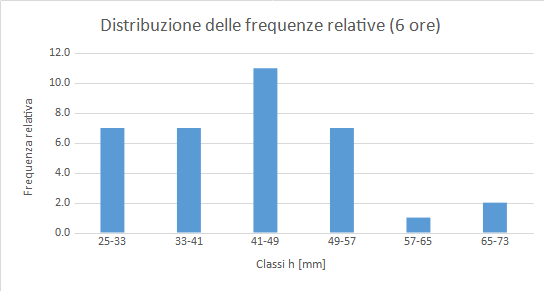
\includegraphics[scale=.6]{immagini/freq_piogg_rel_6ore.png}
        \caption{Distribuzione delle frequenze relative di pioggia (suddivise per classi omogenee), di un evento di durata 6 ore.}
      \label{freq_rel_piogg_05ore}
\end{figure}
    
\begin{figure}[H]\centering
        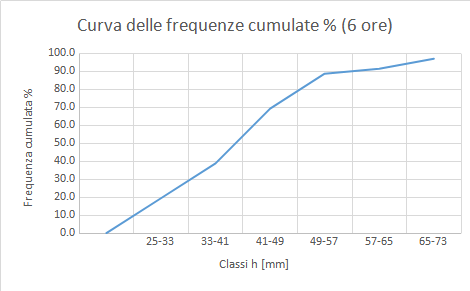
\includegraphics[scale=.6]{immagini/freq_piogg_cum_6ore.png}
        \caption{Frequenze di pioggia cumulata, relative ad un evento di durata 6 ore.}
      \label{freq_cum_piogg_05ore}
\end{figure}    

\begin{table}[H] \centering
    \caption{\textcolor{red}{Valori di altezza di pioggia attesa (teorica), calcolata mediante la variabile d'appoggio $y$ di Weibull o di Hazen.}}
    \begin{tabular}{cccc}
 & & \multicolumn{2}{c}{$h = Y/\alpha + u$}       \\
 \toprule
    \textbf{n} & \textbf{h (mm)  6 ore} & \textbf{h mediante Weibull} & \textbf{h mediante Hazen} \\
\midrule
    1          & 25                          & 27.245                & 25.823                 \\
    2          & 26.4                        & 29.033                & 28.315                 \\
    3          & 26.8                        & 30.285                & 29.782                 \\
    4          & 27.8                        & 31.302                & 30.910                 \\
    5          & 30.4                        & 32.185                & 31.863                 \\
    6          & 32.6                        & 32.981                & 32.709                 \\
    7          & 32.8                        & 33.719                & 33.485                 \\
    8          & 33                          & 34.414                & 34.211                 \\
    9          & 33.6                        & 35.079                & 34.901                 \\
    10         & 35.6                        & 35.721                & 35.566                 \\
    11         & 37.2                        & 36.347                & 36.213                 \\
    12         & 37.6                        & 36.963                & 36.847                 \\
    13         & 37.8                        & 37.571                & 37.473                 \\
    14         & 38.4                        & 38.176                & 38.095                 \\
    15         & 39.4                        & 38.782                & 38.716                 \\
    16         & 41.8                        & 39.390                & 39.341                 \\
    17         & 41.8                        & 40.005                & 39.971                 \\
    18         & 42.2                        & 40.628                & 40.611                 \\
    19         & 42.6                        & 41.263                & 41.263                 \\
    20         & 44.4                        & 41.913                & 41.931                 \\
    21         & 44.8                        & 42.582                & 42.618                 \\
    22         & 45                          & 43.272                & 43.329                 \\
    23         & 46.6                        & 43.990                & 44.069                 \\
    24         & 47.2                        & 44.738                & 44.842                 \\
    25         & 48                          & 45.525                & 45.657                 \\
    26         & 48.8                        & 46.357                & 46.520                 \\
    27         & 50.6                        & 47.242                & 47.442                 \\
    28         & 51.4                        & 48.194                & 48.437                 \\
    29         & 51.4                        & 49.226                & 49.521                 \\
    30         & 51.8                        & 50.359                & 50.719                 \\
    31         & 52.8                        & 51.622                & 52.065                 \\
    32         & 53.2                        & 53.055                & 53.610                 \\
    33         & 55.6                        & 54.723                & 55.436                 \\
    34         & 58.2                        & 56.734                & 57.687                 \\
    35         & 65.4                        & 59.287                & 60.654                 \\
    36         & 71.6                        & 62.833                & 65.093                 \\
    37         & 130.2                       & 68.809                & 74.499       \\
    \bottomrule         
    \end{tabular}
    \end{table}

\begin{figure}[H]\centering
        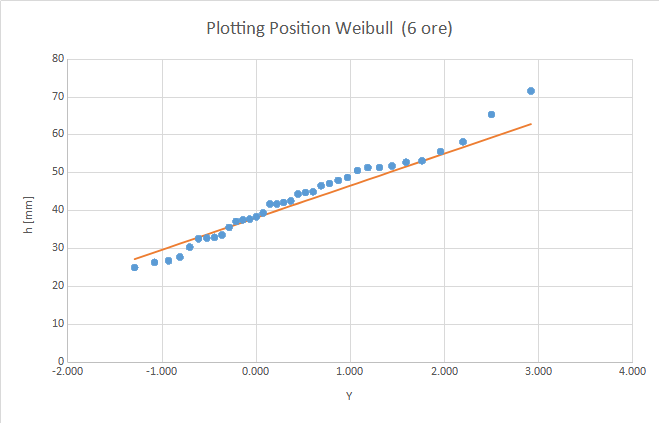
\includegraphics[scale=.5]{immagini/plot_pos_weib_6ore.png}
        \caption{Plotting position mediante Weibull.}
      \label{plot_pos_weib_6ore}
 \end{figure}

\begin{figure}[H]\centering
        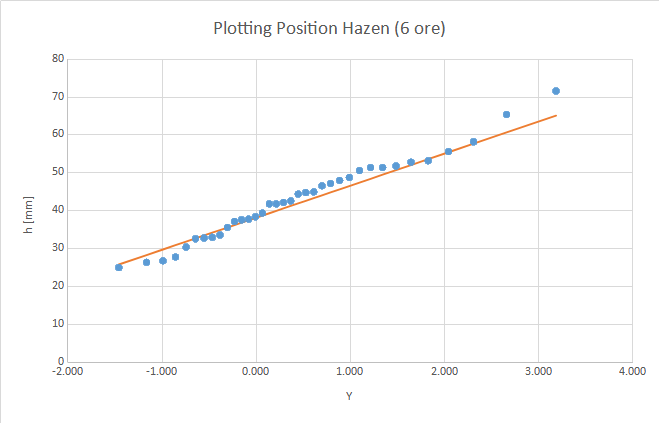
\includegraphics[scale=.5]{immagini/plot_pos_hazen_6ore.png}
        \caption{Plotting position mediante Hazen.}
      \label{plot_pos_hazen_6ore}
\end{figure}

\begin{table}[H] \centering
    \caption{\textcolor{red}{Altezze di pioggia attese per il $T_r$ di riferimento e durata di 6 ore.}}
        \begin{tabular}{ccc}
        \toprule
        Tr (anni) & y     & h attesa (mm) \\
        \midrule
        2 & 0.367 & 41.3  \\
        5 & 1.500 & 50.8  \\
        10  & 2.250 & 57.2          \\
        30  & 3.384 & 66.8          \\
        50  & 3.902 & 71.2          \\
        100 & 4.600 & 77.1          \\
        200 & 5.296 & 82.9          \\         
        \bottomrule
        \end{tabular}
\end{table}

\begin{table}[H] \centering
    \caption{\textcolor{red}{Parametri per l'esecuzione del test statistico di Matalas, relativi alla durata di precipitazione di 6 ore.}}
    \begin{tabular}{cc}
    \toprule
    media                  & 43.04 \\
    $N ^{0.5}$             &  6.000\\
    G                      & 0.434 \\
    G - E                  &  0.447\\
    2 $\sigma$             & 1.069 \\
    TEST                   & Vero \\
    \bottomrule
    \end{tabular}
\end{table}

\subsection{LSPP - Linee segnalatrici di probabilità pluviometrica}
Dopo aver ottenuto le quantità di precipitazioni teoriche, per ogni durata di evento pluviometrico e per diversi tempi di ritorno, è possibile creare un grafico che metta in relazione tutti questi parametri.

\begin{table}[H]\centering
    \caption{\textcolor{red}{Tabella riassuntiva delle altezze di pioggia previste per determinate durate e per determinati tempi di ritorno.}}
    \begin{tabular}{ccccccc}
    \toprule
    \multirow{2}{*}{\textbf{durata t (ore)}} & \multicolumn{6}{c}{\textbf{Altezza di pioggia attesa h (mm) per Tr}} \\
  & \textbf{2 anni} & \textbf{5 anni} & \textbf{30 anni} & \textbf{50 anni} & \textbf{100 anni} & \textbf{200 anni} \\
    \textbf{0.5}                             & 19.83           & 25.30           & 34.38            & 36.88            & 40.25             & 43.60             \\
    \textbf{1}                               & 24.05           & 30.69           & 41.75            & 44.78            & 48.88             & 52.96             \\
    \textbf{3}                               & 32.38           & 41.50           & 56.67            & 60.84            & 66.46             & 72.06             \\
    \textbf{6}                               & 41.26           & 50.85           & 66.78            & 71.16            & 77.06             & 82.94            \\
    \bottomrule
    \end{tabular}
    \label{altezze_critiche_pioggia}
    \end{table}

La curva interpolatrice ha un andamento caratteristico che segue la funzione $h=at^n$, con $a$ che dipende dal tempo di ritorno T e con $n$ che risulta essere una costante per la stazione di rilevamento dei dati (in Italia generalmente è tra 0.20 e 0.55). Il parametro $n$ è un valore sempre inferiore ad 1 perchè all'aumentare del tempo dell'evento pluviometrico, l'intensità di pioggia cala.\\
Essendo che:
\begin{equation}
    h=at^n \rightarrow \log h = \log a + n \log t \rightarrow H=A+nT
    \label{formula_LSPP}
\end{equation}
Mediante l'equazione $H = \log h$, possiamo calcolare il valore di H della tabella \ref{altezze_critiche_pioggia}:

\begin{table}[H] \centering
    \caption{\textcolor{red}{Tabella riassuntiva delle altezze di pioggia previste per determinate durate e per determinati tempi di ritorno, in scala logaritmica.}}
    \begin{tabular}{ccccccc}
        \toprule
    \multirow{2}{*}{\textbf{T}} & \multicolumn{6}{c}{\textit{\textbf{H = log h}}}                                                            \\ & \textbf{2 anni} & \textbf{5 anni} & \textbf{30 anni} & \textbf{50 anni} & \textbf{100 anni} & \textbf{200 anni} \\
    \textbf{-0.301}             & 1.297           & 1.403           & 1.536            & 1.567            & 1.605             & 1.639             \\
    \textbf{0.000}              & 1.381           & 1.487           & 1.621            & 1.651            & 1.689             & 1.724             \\
    \textbf{0.477}              & 1.510           & 1.618           & 1.753            & 1.784            & 1.823             & 1.858             \\
    \textbf{0.778}              & 1.616           & 1.706           & 1.825            & 1.852            & 1.887             & 1.919  \\
    \bottomrule          
    \end{tabular}
    \end{table}
Nel caso in cui gli assi del grafico avessero entrambi la scala logaritmica, la linea interpolatrice dei punti sarebbe una retta.\\
Invertendo la formula della LSPP \ref{formula_LSPP}, è possibile calcolarsi i valori dei rimanenti parametri:
\begin{table}[H] \centering
    \begin{tabular}{ccccccc}
    \toprule
 & \textbf{2 anni} & \textbf{5 anni} & \textbf{30 anni} & \textbf{50 anni} & \textbf{100 anni} & \textbf{200 anni} \\
    \textit{A} & 1.382  & 1.487  & 1.620  & 1.650  & 1.688  & 1.722  \\
    \textit{a} & 24.080 & 30.679 & 41.647 & 44.659 & 48.722 & 52.771 \\
    \textit{n} & 0.291  & 0.280  & 0.269  & 0.267  & 0.264  & 0.262  \\
    \bottomrule
    \end{tabular}
    \end{table}
Riassumendo, le equazioni delle LSPP per la nostra area di studio, possiedono i parametri numerici:

\begin{table}[H] \centering
    \caption{\textcolor{red}{Parametri a e n per poter ricavare la funzione LSPP, dato un certo tempo di ritorno e di durata di pioggia.}}
    \begin{tabular}{ccc}
    \toprule
    \multirow{2}{*}{\textbf{Tempo di ritorno (anni)}} & \multicolumn{2}{c}{\textbf{LSPP}} \\
     & \textbf{a}      & \textbf{n}      \\
    2                                                 & 24.080          & 0.291           \\
    5                                                 & 30.679          & 0.280           \\
    30                                                & 41.647          & 0.269           \\
    50                                                & 44.659          & 0.267           \\
    100                                               & 48.722          & 0.264           \\
    200                                               & 52.771          & 0.262   \\
    \bottomrule  
    \label{parametri_LSPP}     
    \end{tabular}
    \end{table}

Per le durate di precipitazione già studiate in questa relazione (0.5, 1, 3 e 6 ore), la LSPP attribuisce le seguenti altezze di pioggia:

\begin{table}[H]\centering
    \caption{\textcolor{red}{Calcolo per le principali durate temporali dell'altezza di precipitazione prevista per un dato tempo di ritorno (mediante l'equazione LSPP).}}
    \begin{tabular}{ccccccc}
        \toprule
    \multirow{2}{*}{\textbf{$T_p$ (ore)}} & \multicolumn{6}{c}{\textit{\textbf{h calcolata (mm)}}}  \\
    & \textbf{Tr=2anni} & \textbf{Tr=5anni} & \textbf{Tr=30anni} & \textbf{Tr=50anni} & \textbf{Tr=100anni} & \textbf{Tr=200anni} \\
    \textbf{0.5}                           & 19.68                & 25.27                & 34.56                 & 37.12                 & 40.56                  & 44.00                  \\
    \textbf{1}                             & 24.08                & 30.68                & 41.65                 & 44.66                 & 48.72                  & 52.77                  \\
    \textbf{3}                             & 33.15                & 41.72                & 55.96                 & 59.87                 & 65.14                  & 70.40                  \\
    \textbf{6}                             & 40.55                & 50.66                & 67.43                 & 72.04                 & 78.25                  & 84.43           \\
    \bottomrule      
    \end{tabular}
    \end{table}

Conoscendo i parametri delle funzioni matematiche delle LSPP, è possibile vedere graficamente l'andamento di tali curve, creando un apposito grafico.

\begin{figure}[H]\centering
        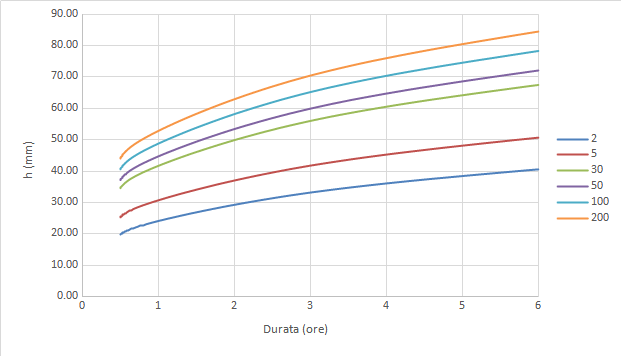
\includegraphics[scale=.75]{immagini/LSPP.png}
        \caption{Grafico della LSPP per ogni tempo di ritorno studiato, in anni.}
      \label{LSPP}
\end{figure}


\section{Calcolo delle portate di progetto (analisi dei deflussi di piena)}
Al fine di conoscere la quantità di deflusso prevista alla sezione di chiusura, occorre prima ricavarsi dei parametri fisici del bacino.

\subsection{Calcolo del tempo di corrivazione del bacino}
Il tempo di corrivazione di un bacino è il tempo che impiega una particella d'acqua ad arrivare alla sezione di chiusura, partendo dal punto idraulicamente più distante da essa.\\
La conoscenza del tempo di corrivazione del bacino permette di prevedere il momento in cui avviene il picco di deflusso alla sezione di chiusura.\\
Esistono diverse metodologie per calcolare il tempo di corrivazione del bacino: metodo cinematico, metodo empirico di Giandotti, di Ferro,...
\subsubsection{Metodo cinematico}
Il metodo cinematico per il calcolo del tempo di corrivazione del bacino implica lo studio del moto dell'acqua sia nel tratto di versante e sia nel tratto di reticolo idrografico.
\begin{equation}
    T_c = T_v + T_r
    \label{tempo_corrivazione}
\end{equation}
Dove:
\begin{itemize}
    \item $T_c$: tempo di corrivazione;
    \item $T_v$: tempo di versante;
    \item $T_r$: tempo di reticolo.
\end{itemize}
Sia per il calcolo del movimento dell'acqua nel reticolo e sia per quello nel versante, è necessario conoscere alcune quote altimetriche del bacino:
\begin{itemize}
    \item $h_0$ (quota della sezione di chiusura): 1183 m s.l.m.;
    \item $h_r$ (quota superiore del collettore principale): 1883 m s.l.m.;
    \item $h_s$ (quota massima del bacino): 2084.3 m s.l.m. 
\end{itemize}
Partendo dalla formula generale della velocità di un fluido: 
\begin{equation}
    V = K_s \cdot R_h^{\frac{2}{3}} \cdot i ^{\frac{1}{2}}
\end{equation}
e svolgendo alcune semplificazioni, è possibile ottenere le formule per il calcolo della velocità nel reticolo e nel versante:
\begin{equation}
    V_R \approx (5 - 10) \cdot i^{\frac{1}{2}}
    \label{vel_reticolo}
\end{equation}
\begin{equation}
    V_v \approx (0.1 - 0.15) i_v^{\frac{1}{2}}
    \label{vel_versante}
\end{equation}
La formula del tempo di corrivazione \ref{tempo_corrivazione} può essere implementata con le formule \ref{vel_versante} e \ref{vel_reticolo}:
\begin{equation}
    T_c = \frac{L_R}{V_R}+ \frac{L_V}{V_V} \approx \frac{L_R}{(5 - 10) \cdot i^{\frac{1}{2}}} + \frac{L_V}{(0.1 - 0.15) i_v^{\frac{1}{2}}}
\end{equation}

Per il calcolo della velocità di reticolo dell'acqua nel bacino, è necessario imporre un valore di pendenza del retico; questo valore si ricava dal rapporto tra la differenza di quota del collettore principale (1883 m-1183 m) e la sua lunghezza (2401 m).\\
Svolgendo la formula \ref{vel_reticolo}, imponendo un coefficiente medio di 7.5, il risultato è $4.05 \frac{m}{s}$.\\
Conoscendo la lunghezza del collettore principale, è possibile ricavare il tempo di corrivazione della componente del reticolo idrografico.\\
In modo analogo, il calcolo della velocità dell'acqua nel versante avviene conoscendo la pendenza del tratto di terreno, ovvero il rapporto tra la differenza di quota (2084.3 m-1883 m) e la sua distanza, ricavata dal GIS, di 445.16 m.\\
Applicando la formula \ref{vel_versante}, applicando un coefficiente di 0.1, la velocità di versante risulta essere di $0.07 \frac{m}{s}$.\\
Anche in questo caso, il tempo di corrivazione nel versante è ricavabile invertendo la formula della velocità.
I tempi di percorrenza dell'acqua sono:
\begin{table}[H] \centering
    \begin{tabular}{ccc}
        \toprule
    \textbf{$T_v$} & \textbf{$T_r$} & {\color[HTML]{000000} } \\
    6619.91     & 592.90      & sec                     \\
    1.84        & 0.16        & ore       \\
    \bottomrule             
    \end{tabular}
    \end{table}
Il tempo di corrivazione totale, ovvero la somma dei due parziali, risulta essere pari a 120.21 minuti (ovvero 2 ore).

\subsubsection{Metodo empirico di Giandotti}
Il metodo di Giandotti, per il calcolo del tempo di corrivazione del bacino, richiede l'applicazione della relativa formula:
\begin{equation}
    T_c = \frac{4 \cdot \sqrt{A}+ 1.5 \cdot L}{0.8 \cdot \sqrt{H_m}}
\label{formula_giandotti}
\end{equation}
Dove: 
\begin{itemize}
    \item $T_c$: è il tempo di corrivazione, espresso in ore;
    \item A: è l'area del bacino, espressa in $km^2$;
    \item L: è lunghezza del collettore idraulico, estesa fino allo spartiacque, espressa in km;
    \item $H_m$: è l'altezza media del bacino, riferita alla sezione di chiusura ed espressa in m.
\end{itemize}
Per il bacino in esame:
\begin{itemize}
    \item A: 2.01 $km^2$;
    \item $L_c$: 2.846 $km$;
    \item $H_m$: 470.9 $m$.
\end{itemize}
La formula di Giandotti \ref{formula_giandotti}, con i parametri del bacino in esame, restituisce il tempo di corrivazione di 34.4 minuti (0.573 ore).\\
Questa formula notoriamente restituisce valori di corrivazione molto contenuti rispetto a quelli reali.

\subsubsection{Metodo empirico di Ferro (I)}
La formula necessaria da applicare per questo metodo è la seguente:
\begin{equation}
    T_c = 0.022 \cdot \left(\frac{L_C}{i^{0.5}}\right)^{0.8}
    \label{formula_ferro_I}
\end{equation}
Dove: 
\begin{itemize}
    \item $T_c$: viene espressa in minuti;
    \item $L_C$: viene espressa in metri;
    \item i: viene espressa $\frac{m}{m}$.
\end{itemize}
Nel caso del bacino in esame:
\begin{itemize}
    \item A: 2.01 $km^2$;
    \item $L_C$: 2401 $m$;
    \item $i_r$: 0.293 $\frac{m}{m}$.
\end{itemize}
La formula del metodo di Ferro (I) \ref{formula_ferro_I} restituisce il valore di 18.19 minuti.\\
Nel caso di bacini montani con collettore principale corto (qualche chilometro), e ripido, la formula tende a sottostimare il valore reale.

\subsubsection{Metodo empirico di Ferro (II)}
La formula di Ferro (II) richiede solamente la conoscenza dell'area del bacino:
\begin{equation}
    T_c = 0.675 \cdot \sqrt{A}
    \label{formula_ferro_II}
\end{equation}
Dove:
\begin{itemize}
    \item $T_c$: viene espressa in ore;
    \item $A$: viene espressa in $km^2$.
\end{itemize}
Nel caso del nostro bacino, come già riportato prima, l'area è pari a 2.01 $km^2$.\\
La formula \ref{formula_ferro_II} restituisce un tempo di corrivazione pari a 57.42 minuti (0.96 ore).

\subsection{Comparazione dei metodi di corrivazione}
Dopo aver applicato diversi metodi per il calcolo del tempo di corrivazione, risulta utile compararli.
\begin{table}[H] \centering
    \caption{\textcolor{red}{Comparazione dei diversi metodi di calcolo del tempo di corrivazione.}}
    \begin{tabular}{ccc}
        \toprule
  Metodo di calcolo   & $T_c$ in minuti & $T_c$ in ore\\
     \midrule
   Cinematico  & 120.21 & 2.00\\
   Giandotti  & 34.356 & 0.573\\
   Ferro (I)  & 18.19 & 0.30\\
   Ferro (II)  &57.42 & 0.96\\
     \bottomrule
    \end{tabular}
    \end{table}
\section{Definizione dell'intervento di sistemazione e trasporto solido atteso}
Al fine di dimensionare le opere idrauliche da poter costruire all'interno del bacino idraulico, è necessario studiare le caratteristiche morfologiche del bacino stesso e del reticolo idraulico che lo attraversa.\\
Infatti, il processo erosivo prodotto dal reticolo idraulico dipende da:
\begin{itemize}
    \item tipologia del corso d'acqua alluvionale ed i suoi gradi di libertà (incisione ed allargamento);
    \item forma di trasporto solido prevalente: di fondo, iperconcentrato, colate detritiche,...;
    \item tipo di torrente: di scavo o di trasporto.
\end{itemize}
Il trasporto solido generato dalla corrente può essere:
\begin{itemize}
    \item ``bedload" (di fondo): comprende lo strisciamento, rotolamento o saltellamento dei sedimenti del letto del fiume;
    \item ``suspended load" (in sospensione): è generato dai vortici di turbolenza del flusso d'acqua, e trasporta generalmente il materiale di piccole dimensioni.
\end{itemize} 
\subsubsection{Equilibrio e dinamica del torrente}
Le modificazioni che si verificano in un corso d'acqua sono il risultato della sua tendenza a trovare uno stato di equilibrio.\\
Questo concetto può essere compreso considerando la ``Bilancia di Lane" (1955), ovvero una rappresentazione grafica che permette di capire come sarà il comportamento di un corso d'acqua al fine di raggiungere il proprio equilibrio.
\begin{figure}[H]  \centering
    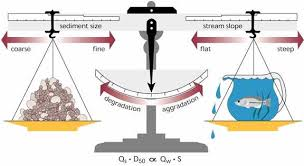
\includegraphics[scale=1]{immagini/bilancia_lane.jpg}
    \caption{Bilancia di Lane}
    \label{bilancia_lane}
\end{figure}
Matematicamente, il comportamento di un torrente al fine di ottenere l'equilibrio può essere riportato con questa formula:
\begin{equation}
    Q_L \cdot S \overset{=}{\propto} Q_S \cdot D_{50}
    \label{bilancia_lane}
\end{equation}
Dove:
\begin{itemize}
    \item $Q_L$ è la portata liquida del corso d'acqua;
    \item $S$ è la pendenza del thalweg;
    \item $Q_S$ indica la portata solida di sedimenti trasportata;
    \item $D_{50}$ indica il valore mediano della serie granulometrica rilevata nell'alveo.
\end{itemize}
La formula \ref{bilancia_lane} può anche essere considerata come se al primo membro fosse rappresentata la ``stream power" del fiume ed al secondo membro fosse riportato l'attrito al movimento.\\
Secondo la ``Classificazione di Horatiis" (1930), i tratti fluviali di montagna possono essere suddivisi in:
\begin{itemize}
    \item torrenti di trasporto: l'energia della corrente è tale da essere completamente impegnata nel trasporto di materiale solido a valle; il letto tende a non abbassarsi o ad alzarsi. Le opere progettate per questi tratti hanno l'obiettivo di trattenere il sedimento;
    \item torrenti di scavo: l'energia della corrente produce trasporto solido ed incisione del letto; il letto tende ad abbassarsi, generando una tendenza all'incisione verso monte. Le opere progettate per questi tratti hanno l'obiettivo di consolidare maggiormente i tratti dove l'opera di erosione ha una maggiore presenza.
\end{itemize}

\subsection{Briglie di consolidamento}
Mediante le briglie di consolidamento si vuole indurre il tratto di reticolo verso una pendenza di equilibrio dinamico del profilo ($i_c$) \ref{profilo_briglia_consolidamento}.\\
La pendenza $i_c$ equivale alla pendenza che è necessario assegnare ad un certo tratto fluviale, affinché si trovi nelle condizioni di mettere in mobilità una precisa quantità granulometrica di sedimento al fondo.\\
Le briglie di consolidamento possono essere di tipo longitudinale (per la stabilizzazione delle sponde) o di tipo trasversale (al fine di ridurre o controllare la pendenza longitudinale del profilo.)
In molti casi, se necessario, vengono erette in successione una serie di briglie di consolidamento.

\begin{figure}[H] \centering
    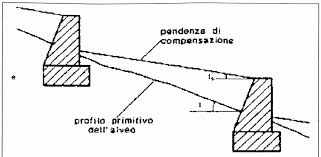
\includegraphics[scale=1]{immagini/profilo_briglia_consolidamento.jpg}
    \caption{Profilo di una briglia di consolidamento, con riportata la pendenza originaria e quella che si manifesta successivamente alla costruzione dell'opera.}
    \label{profilo_briglia_consolidamento}
\end{figure}

Il dimensionamento ed ulteriori informazioni su queste opere idrauliche verranno riportate più approfonditamente nel capitolo successivo.

\subsection{Studio della granulometria}
Con il termine ``granulometria" s'intende la proprietà con cui è possibile descrivere e studiare un insieme di particelle del suolo, siano queste sabbiose, ghiaiose,...\\
Lo studio granulometrico permette di conoscere, in modo statistico, la composizione del terreno di studio.\\
L'analisi granulometrica inizia andando a misurare, in modo sistematico, la grandezza (generalmente il diametro) dei clasti presenti nel letto dell'alveo o nelle barre.\\
Successivamente, si procede alla suddivisione in classi dei diametri misurati, per poi andare a calcolare la frequenza relativa, cumulata e percentuale per ognuna.\\
Per il caso di studio di questa relazione, la curva che interpola la frequenza cumulata e la classe diametrica dei sedimenti è la seguente.
\begin{figure}[H] \centering
    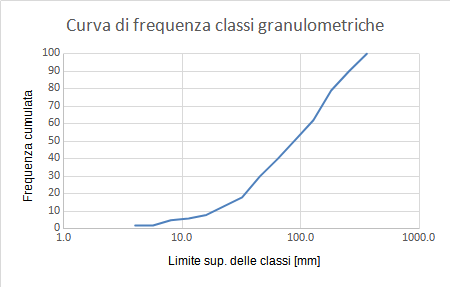
\includegraphics[scale=0.75]{immagini/curva_freq_classi_granuometriche.png}
    \caption{Curva della frequenza cumulata delle classi granulometriche.}
    \label{curva_freq_classi_granulometriche}
\end{figure}
Infine, per conoscere la distribuzione statistica delle grandezze dei  sedimenti, all'interno del campione rilevato, è necessario applicare la seguente formula:
\begin{equation}
D_\% = \left[\frac{D_2-D_1}{F_2-F_1}\right] \cdot (F-F_1)+D
\end{equation} 
Dove:
\begin{itemize}
    \item $D$ indica la classe diametrica;
    \item $F$ indica la frequenza cumulata.
\end{itemize}
Per il caso di studio inerente a questa relazione, i risultati sono:
\begin{table}[H]\centering
    \caption{\textcolor{red}{Classi di frequenza cumulata inerente ai sedimenti del bacino idrografico di studio. I valori relativi ai diametri sono espressi in $mm$.}}
    \begin{tabular}{cc}
    \toprule
    N   & 100      \\
    \midrule
    D16 & 28.25    \\
    D50 & 88.10    \\
    D84 & 215.10   \\
    D90 & 256.00   \\
    \bottomrule
    \end{tabular}
    \end{table}

\subsection{Calcolo della pendenza di correzione}
\subsubsection{Approccio statico per la stima di $i_c$}
Secondo Fattorelli et al. (1980), basandosi su 1000 tratti sistemati in Trentino, il valore $i_c$ può essere calcolato mediante le seguenti formule:
\begin{itemize}
    \item per bacini mediamente erodibili:
\begin{equation}
    i_c = 0.66 \cdot i_0 
\end{equation}
\item per bacini poco erodibili
\begin{equation}
    i_c = 0.77 \cdot i_0 
\end{equation}
\item per bacini molto erodibili
\begin{equation}
    i_c = 0.59 \cdot i_0 
\end{equation}
\end{itemize}
 
Secondo Heede (1960), il calcolo di $i_c$ avviene mediante:
\begin{equation}
    i_c = (0.6 - 0.7) \cdot i_0
\end{equation}

\subsubsection{Approccio mediante lo sforzo tangenziale medio}
Considerando le condizioni di moto uniforme ($i_F=i_E=i$), la corrente esercita sul contorno uno sforzo tangenziale medio, con formula:
\begin{equation}
    \tau = \gamma \cdot R_H \cdot i
\end{equation}
Conoscendo la $i_c$, ovvero la pendenza che si ambisce ad ottenere successivamente alla costruzione dell'opera, è possibile calcolare la $\tau_{c}$, mediante la formula precedentemente riportata.\\
Lo sforzo massimo che si genera nel letto del fiume, ha valore calcolabile mediante la formula:
\begin{equation}
    \tau_{max} = \gamma \cdot y \cdot i
\end{equation}
Mentre, per quanto riguarda lo sforzo agente sulle sponde, il calcolo avviene mediante:
\begin{equation}
    \tau_{sponde-fondo-max}= K \cdot (\gamma, y, i)
\end{equation}
Secondo le ricerche Shields (1936), e successive semplificazioni, la relazione tra sforzo al fondo e grandezza dei sedimenti è regolata dalla formula:
\begin{equation}
    \tau_c \approx 1000 \cdot D
    \label{tau_cr_shields}
\end{equation}
\subsubsection{Approccio deterministico per la stima di $i_c$}
Secondo Shields (1936), la formula per il calcolo dello sforzo tangenziale critico è:
\begin{equation}
    \tau_c = 0.06 \cdot (\gamma_s -\gamma) \cdot D
\end{equation}
Dove:
\begin{itemize}
   \item $D$ è la taglia granulometrica di riferimento;
    \item $\gamma_s$ è il peso specifico dei sedimenti;
    \item $\gamma$ è il peso specifico dell'acqua.
\end{itemize}
Tale formula può anche essere riscritta, diventando:
\begin{equation}
    i_c = \frac{\tau_c^* \cdot (\gamma_s-\gamma) \cdot D}{\gamma \cdot Rh}
\end{equation}

\subsubsection{Soluzione esplicita semplificata per sezioni rettangolari molto larghe}
Nel caso in cui il corso d'acqua dovesse passare attraverso una sezione rettangolare ampia e con un tirante idraulico ridotto, è possibile adottare alcune approssimazioni e semplificazioni.\\
Data una sezione rettangolare, potendo trascurare l'altezza del tirante idraulico $h$, il raggio idraulico $Rh$ risulta essere:
\begin{equation}
    \frac{B \cdot h}{B + 2\cdot h} \approx \frac{B \cdot h}{B} \approx h
\end{equation}
La formula per il calcolo del coefficiente di scabrezza $ks$, conoscendo il parametro relativo alla granulometria $D_{90}$ è:
\begin{equation}
K_s \approx \frac{26}{D_{90}^{1/6}}
\end{equation}
Essendo che la portata $Q$ è calcolabile come il prodotto dell'area per la velocità, è possibile esplicitare tutte e due le componenti della formula, che diventa:
\begin{equation}
    Q = (Ks \cdot Rh^{2/3} \cdot \sqrt{i_c}) \cdot (B \cdot h)
    \label{portata_sez_rett}
\end{equation}
Dove:
\begin{itemize}
    \item Ks è il coefficiente di scabrezza del fondo $\left[\frac{m^{1/3}}{s^{-1}}\right]$;
    \item Rh indica il raggio idraulico $[m]$;
    \item $i_c$ è la pendenza di correzione $\left[m/m\right]$;
    \item B è la larghezza dell'alveo $[m]$;
    \item h è la profondità del tirante idraulico $[m]$.
\end{itemize}
Sostituendo alla formula \ref{portata_sez_rett} il raggio idraulico, la formula diventa:
\begin{equation}
    Q = (Ks \cdot h^{2/3} \cdot \sqrt{i_c}) \cdot (B \cdot h)
\end{equation}
Che diventa:
\begin{equation}
    Q = (Ks \cdot h^{5/3} \cdot \sqrt{i_c}) \cdot B
\end{equation}

Il procedimento prosegue mediante il calcolo della pendenza di correzione:
\begin{equation}
    i_c = \left(\frac{0.1 \cdot D_{90} \cdot ks^{0.6} \cdot B^{0.6}}{Q^{0.6}_{30}} \right) ^{1.43}
    \label{pend_critica_iterativo}
\end{equation}
La profondità del tirante relativo alla condizione critica è calcolabile mediante la formula:
\begin{equation}
    h_c = \left( \frac{Q}{ks \cdot B \cdot \sqrt{i}}\right)^{3/5}
\end{equation}
Nel caso in cui il rapporto tra $h_c$ e $D_{84}$ è minore a 3.5, è possibile iniziare il procedimento di calcolo iterattivo mediante la formula di Barhurst (1985):
\begin{equation}
    Ks= \frac{\sqrt{g}}{h^{1/6}} \left[5.62 \cdot \log \left(\frac{h}{D_{84}}\right)+4\right]
    \label{ks_scabrezza_barhurst}
\end{equation}
Dal valore di scabrezza calcolato è possibile ricavare il valore di pendenza critica, sempre mediante la formula \ref{pend_critica_iterativo}. Il procedimento iterativo termina quando il valore di scabrezza ks non si discosta molto da quello ricavato precedentemente.

\subsection{Determinazione di altezza e numero di briglie di consolidamento}
Successivamente ad aver calcolato la pendenza di correzione più ottimale per il caso di studio, è necessario valutare le misure di massima delle briglie, quali altezza, numero ed interdistanza tra ciascuna.\\
Come primo passaggio è necessario calcolare la variazione di quota totale per tutto il tratto, ed avviene mediante la formula:
\begin{equation}
    \Delta Z = (i_0 - i_c) \cdot L_s
\end{equation}
Successivamente, è necessario porre un'altezza di primo tentativo della briglia. Utilizzando questo valore per dividere la differenza di quota totale, è possibile calcolare il numero di opere in serie da costruire.\\
Infine, dividendo la distanza totale del tratto per il numero di opere da ereggere, si ricava l'interdistanza lineare tra una briglia e la successiva.

\subsection{Calcolo della pendenza di correzione per il tratto di studio}
Dopo aver descritto i vari procedimenti per il calcolo della pendenza di correzione, è possibile applicare i concetti per il caso di studio di questa relazione.\\
Dal programma GIS è possibile evidenziare il tratto di reticolo idrografico soggetto alla sistemazione idraulica mediante briglie.
\begin{figure}[H] \centering
    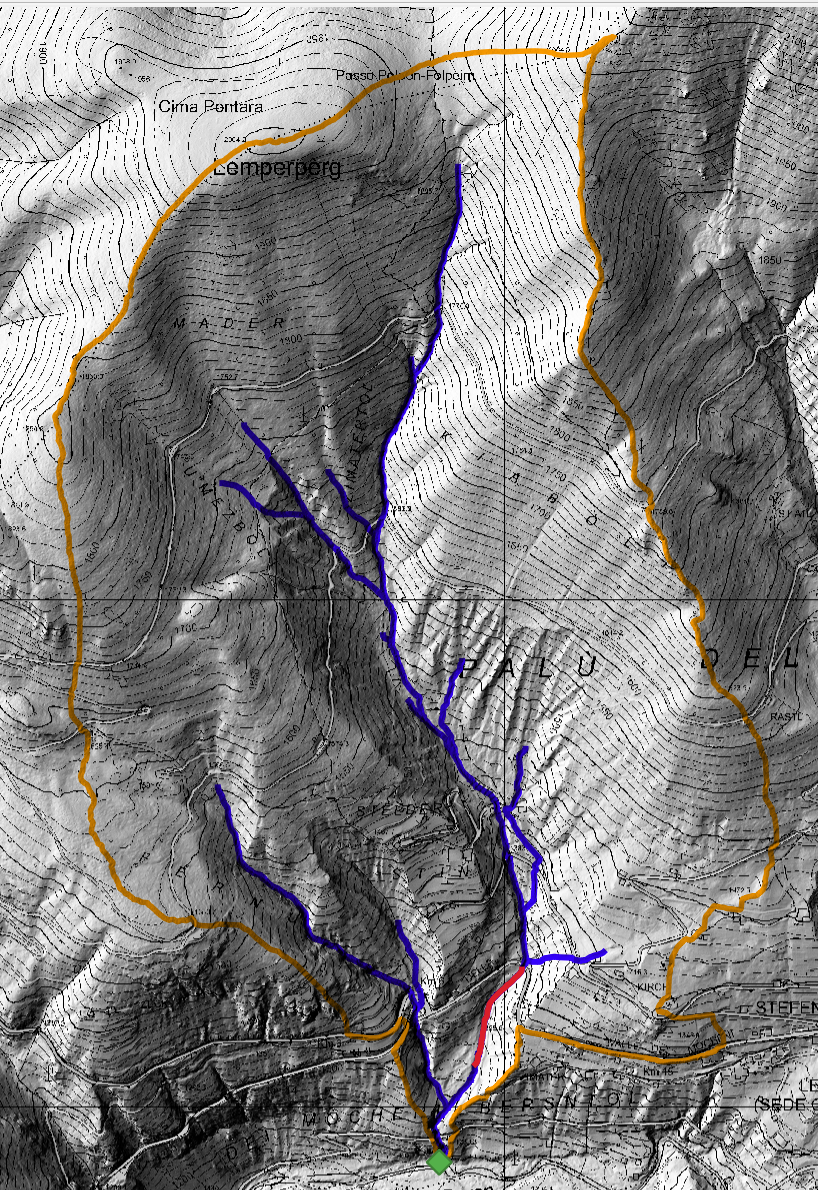
\includegraphics[scale=0.3]{immagini/pendenza_planimetria_1.png}
    \caption{Rappresentazione planimetrica del bacino di studio e del reticolo idrografico, con evidenziato in rosso il tratto interessato dalla sistemazione idraulica.}
    \label{pendenza_planimetria_1}
\end{figure}
\begin{figure}[H] \centering
    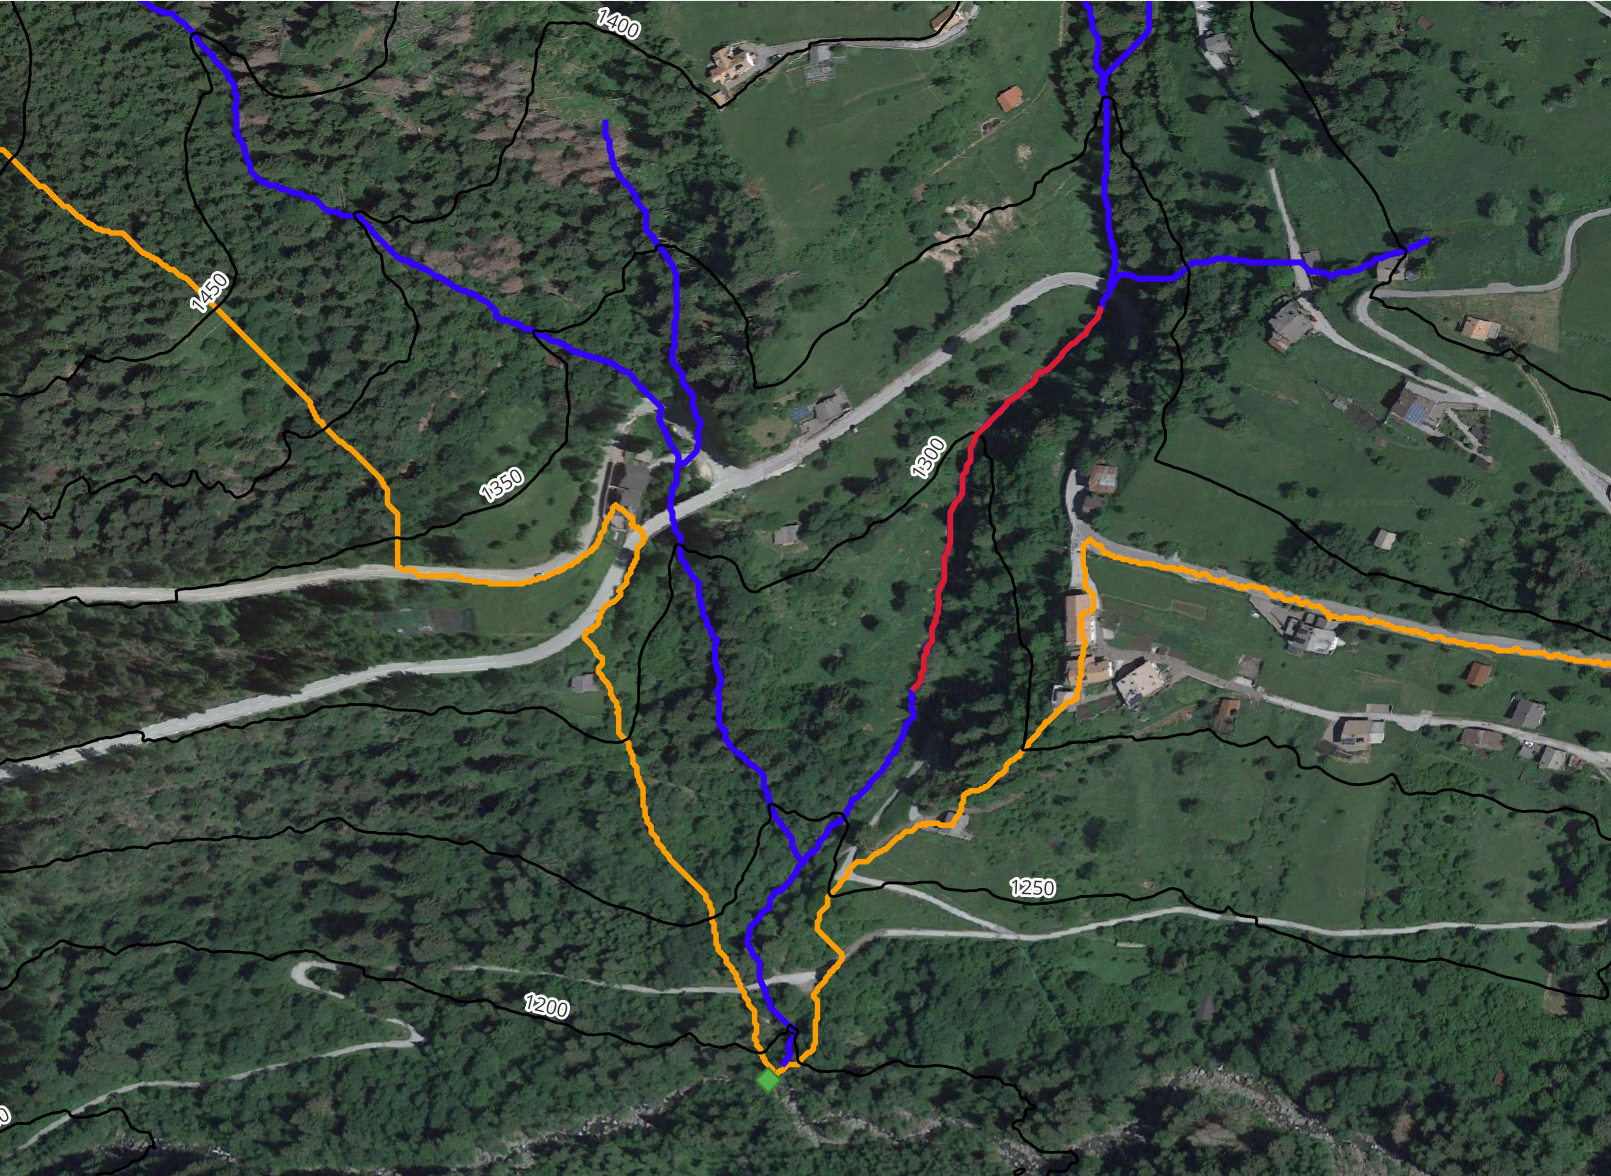
\includegraphics[scale=0.3]{immagini/pendenza_planimetria_2.png}
    \caption{Particolare del bacino di studio, con rappresentazione del tratto soggetto a sistemazione idraulica.}
    \label{pendenza_planimetria_2}
\end{figure}
\begin{figure}[H] \centering
    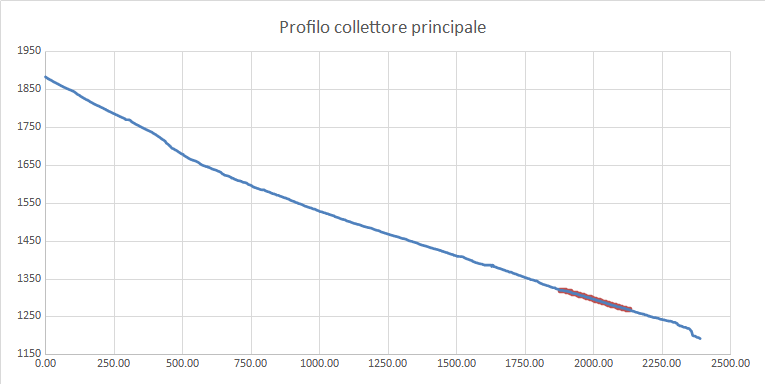
\includegraphics[scale=0.5]{immagini/pendenza_collettore.png}
    \caption{Rappresentazione del profilo del collettore principale, con indicazione del tratto soggetto a sistemazione idraulica (in rosso).}
    \label{pendenza_collettore}
\end{figure}
Mediante dei semplici passaggi matematici, svolti nel programma di calcolo, è possibile ricavarsi le principali informazioni morfologiche inerenti al tratto interessato da sistemazioni:
\begin{table}[H] \centering
    \caption{\textcolor{red}{Principali informazioni morfologiche inerenti al collettore principale del reticolo idrografico e del tratto interessato dalle sistemazioni.}}
    \begin{tabular}{ccc}
    \toprule
                 & collettore & tratto da sistemare \\
    \midrule
    lunghezza    & 2388.27    & 250.83              \\
    pendenza m/m & 0.29       & 0.20                \\
    pendenza °   & 16.12      & 11.57               \\
    \bottomrule
    \end{tabular}
    \label{inf_morf_coll_princ}
\end{table}

Successivamente ad aver svolto per due volte i calcoli iterativi, al fine di ottenere i valori di scabrezza e di pendenza maggiormente ottimali, si è giunti ai seguenti risultati:
\begin{itemize}
    \item ks = 17.0 $m^{1/3}/s$;
    \item $i_c$ = 0.110 $m/m$.
\end{itemize}

Infine, si procede al calcolo del numero di opere in serie da ereggere e le relative interdistanze, imponendo l'altezza del livello inferiore della gaveta.\\
Vengono riportati alcuni risultati.
\begin{table}[H] \centering
    \caption{\textcolor{red}{Serie di risultati inerenti ai valori di numerosità ed interdistanza delle briglie, in funzione dell'altezza imposta.}}
    \begin{tabular}{ccc|ccc}
        \toprule
    Scenario 1 & $\Delta Z$ (m)& 23.68 & Scenario 4 & $\Delta Z$ (m) & 23.68 \\
& Z (m)         & 2.37  &            & Z (m)         & 3.40  \\
& n             & 10  &            & n             & 7  \\
& interdistanza & 25.11 &            & interdistanza & 36.02 \\
\midrule
Scenario 2 & $\Delta Z$ (m)        & 23.68 & Scenario 5 & $\Delta Z$ (m) & 23.68 \\
& Z (m)         & 3.95  &            & Z (m)         & 4.75  \\
& n             & 6   &            & n             & 5   \\
& interdistanza & 41.84 &            & interdistanza & 50.32 \\
    \midrule
Scenario 3 & $\Delta Z$ (m)        & 23.68 & Scenario 6 & $\Delta Z$ (m)        & 23.68 \\
& Z (m)         & 1.70  &            & Z (m)         & 2.63  \\
& n             & 13.9  &            & n             & 9  \\
& interdistanza & 18.01 &            & interdistanza & 27.75 \\
\bottomrule
\end{tabular}
\label{opzioni_numero_altezza_briglie}
\end{table}
La scelta del numero e delle altezze delle briglie verrà fatta successivamente, nel relativo paragrafo.

\subsection{Calcolo preliminare del trasporto solido}
Al fine di studiare la quantità di sedimenti trasportati durante un qualsiasi evento di piena, occorre riuscire a calcolare la relativa capacità massima di trasporto di materiale solido al fondo del corso d'acqua.\\
Shields (1936), grazie ai suoi studi effettuati sul trasporto solido, riuscì a ricavare empiricamente la formula dello sforzo tangenziale critico (necessario a muovere i sedimenti nel letto di un fiume), in funzione del peso specifico dell'acqua, dei sedimenti e della grandezza delle particelle granulometriche.\\
Tale formula, già riportata precedentemente, è la \ref{tau_cr_shields}.\\
Da tale formula è possibile calcolare l'altezza del tirante idraulico che genera lo sforzo tangenziale in grado di muovere i sedimenti, conoscendo il peso volumetrico dell'acqua in movimento e della pendenza del corso:
\begin{equation}
    h_c = \frac{\tau_c}{\gamma \cdot i} 
\end{equation}
Mediante la conoscenza delle pendenze del tratto precedentemente e successivamente alla sistemazione, è possibile valutare come cambia il trasporto solido, calcolato mediante questo procedimento preliminare.\\

\begin{table}[H] \centering
    \caption{\textcolor{red}{Trasporto solido di fondo calcolato nelle condizioni precedenti e posteriori alla sistemazione idraulica del tratto di corso studiato.}}
    \begin{tabular}{cccclccccl}
    \toprule
    \multicolumn{4}{c}{Situazione ANTE SISTEMAZIONE} & & \multicolumn{4}{c}{Situazione POST SISTEMAZIONE} &      \\
    i0 = & 0.205 & & & &ic = & 0.110 & & &      \\
    \midrule
    & $D_{50}$ & $D_{84}$ & $D_{90}$ & & & $D_{50}$ & $D_{84}$ & $D_{90}$ & \\
    \midrule
    & 0.089 & 0.215 & 0.256 & m & & 0.089 & 0.215 & 0.256  & m  \\
    $\tau_c$ & 89 & 215 & 256 & $\frac{N}{m^2}$ & $\tau_c$ & 89 & 215 & 256 & $\frac{N}{m^2}$\\
    $h_c$ & 0.04 & 0.11 & 0.13 & m & $h_c$ & 0.08 & 0.20 & 0.24 & m  \\
   % $Q_c$ & 0.015 & 0.898 & 1.378 & $\frac{m^3}{s}$ & $Q_c$ & 0.32 & 2.71 & 3.90 & $\frac{m^3}{s}$\\
    \bottomrule
    \end{tabular}
    \end{table}
Come previsto, mediante le opere di sistemazione idraulica dei tratti, si incrementa la profondità del tirante idraulico critico necessario a muovere i sedimenti dei letti di torrente.\\
In questo caso, come osservabile nella tabella precedente, il tirante idraulico critico post sistemazione è molto superiore (quasi il doppio) rispetto a quello pre-sistemazione.

\subsection{Calcolo della portata critica di trasporto}
Successivamente ad aver calcolato la profondità del tirante idraulico critico, ovvero necessario a muovere i sedimenti nel letto del corso d'acqua, si procede a calcolare la relativa portata critica, valutando nuovamente la scabrezza, mediante la formula \ref{ks_scabrezza_barhurst}.\\
Il valore di flusso critico si ricava applicando la formula generale della portata idraulica:
\begin{equation}
    Q_c = v_c \cdot A
\end{equation}
Conoscendo la larghezza del torrente di studio (8 metri), è possibile svolgere il calcolo della portata critica, per la condizione precedente e successiva alla sistemazione idraulica del tratto.\\
Per la condizione precedente alla costruzione delle opere idrauliche, con pendenza di 0.205 $m/m$, i calcoli restituiscono i seguenti valori.
\begin{table}[H] \centering
\caption{\textcolor{red}{Valori di portata critica del trasporto solido, nelle condizioni precedenti alla costruzione delle opere idrauliche di correzione della pendenza.}}
\begin{tabular}{ccccccccccc}
\toprule
& h (m) & A $(m^2)$ & C (m) & R (m) & $h/d_{84}$ & Ks& v (m/s)& Qc $(m^3/s)$ \\
\midrule
$D_{50}$& 0.04 & 0.355 & 8.09  & 0.044 & 0.206 & 0.8  & 0.043 & 0.015 \\
$D_{84}$ & 0.11 & 0.857 & 8.21 & 0.104 & 0.498 & 10.4 & 1.048   & 0.898 \\
$D_{90}$ & 0.13  & 1.020  & 8.25 & 0.124 & 0.593 & 12.0 & 1.351 & 1.378 \\
\bottomrule
\end{tabular}
\end{table}

Per quanto riguarda i calcoli nelle condizioni successive alla costruzione delle opere idrauliche, ovvero con pendenza pari a 0.110 $m/m$, i calcoli generano i seguenti valori.
\begin{table}[H] \centering
\caption{\textcolor{red}{Valori di portata critica del trasporto solido, nelle condizioni successive alla costruzione delle opere idrauliche di correzione della pendenza.}}
\begin{tabular}{ccccccccccc}
\toprule
& h (m) & A $(m^2)$ & C (m) & R (m) & $h/d_{84}$ & Ks& v (m/s)& Qc $(m^3/s)$ \\
\midrule
$D_{50}$& 0.08  & 0.658  & 8.16  & 0.081 & 0.383 & 7.9 & 0.487 & 0.320\\
$D_{84}$ & 0.20 & 1.590  & 8.40  & 0.189 & 0.924 & 15.6 & 1.707 & 2.715 \\
$D_{90}$ & 0.24  & 1.893  & 8.47 & 0.223 & 1.101 & 16.9 & 2.059 & 3.898 \\
\bottomrule
\end{tabular}
\end{table}

Come per il sottocapitolo precedente, ed in modo concorde a tali risultati, la portata critica nelle condizioni successive alla sistemazione ha valori nettamente superiori rispetto a quelli della condizione ante-sistemazione.

\subsection{Creazione del sedimentogramma}
Dopo aver calcolato la capacità di trasporto teorica del corso d'acqua, è necessario simulare per un evento di piena (di qualsiasi entità), come varia il trasporto solido. Infatti, il trasporto solido al fondo avviene solamente quando la portata liquida supera quella critica relativa al trasporto solido.\\
Considerando un evento di piena, con tempo di ritorno pari a 200 anni ed utilizzando il metodo del deflusso cinematico, è possibile discretizzare nel tempo la portata liquida e considerare singolarmente come si comporta il trasporto solido.\\
Per questa analisi, si andranno ad utilizzare i dati già ricavati precedentemente, ovvero le portate di deflusso con tempo di ritorno pari a 200 anni (mediante metodo cinematico), lo sforzo cinematico critico per $D_{84}$ ed i valori granulometrici.\\
Il calcolo della portata critica verrà svolta mediante la formula $q_s=2.5 \cdot q \cdot S^{1/6}$, per $q > q_s$.

\begin{table}[H] \centering
    \caption{\textcolor{red}{Portata e volume di materiale solido, nel caso di una piena con tempo di ritorno pari a 200 anni, nella condizione precedente e successiva alla sistemazione idraulica.}}
    \begin{tabular}{ccccc}
        \toprule
& \multicolumn{2}{c}{Sit. ANTE SISTEM.} & \multicolumn{2}{c}{Sit. POST SISTEM.} \\
\midrule
tempo  & $Qs(i_0)$ & $Vs(i_0)$ & $Qs(i_c)$  & $Vs(i_c)$  \\
(minuti) & $(m^3/s)$ & $(m^3)$ & $(m^3/s)$ & $(m^3)$  \\
\midrule
    0     & 0.00 & 0.00 & 0.00 & 0.00   \\
    10    & 0.00 & 0.00  & 0.00  & 0.00                   \\
    20    & 0.00 & 0.00  & 0.00  & 0.00                   \\
    30    & 0.00 & 0.00 & 0.00  & 0.00                   \\
    40    & 0.00 & 0.00& 0.00   & 0.00                   \\
    50    & 0.41 & 243.44  & 0.00       & 0.00                   \\
    60    & 0.86 & 513.26 & 0.32     & 189.57                 \\
    70    & 1.26                   & 754.44                  & 0.46                    & 278.64                 \\
    80    & 1.54                   & 924.60                  & 0.57                    & 341.49                 \\
    90    & 1.68                   & 1006.65                 & 0.62                    & 371.79                 \\
    100   & 1.63                   & 979.41                  & 0.60                    & 361.73                 \\
    110   & 1.41                   & 843.79                  & 0.52                    & 311.64                 \\
    120   & 0.97                   & 582.40                  & 0.36                    & 215.10                 \\
    130   & 0.57                   & 340.30                  & 0.21                    & 125.69                 \\
    140   & 0.38                   & 225.07                  & 0.00                    & 0.00                   \\
    150   & 0.26                   & 153.19                  & 0.00                    & 0.00                   \\
    160   & 0.18                   & 109.01                  & 0.00                    & 0.00                   \\
    170   & 0.00                   & 0.00                    & 0.00                    & 0.00     \\
    \bottomrule             
    \end{tabular}
    \end{table}

Il volume totale dei materiale solido trasportato, nelle condizioni pre-sistemazione è pari a 6675.57 $m^3$, mentre nelle condizioni post-sistemazioni è pari a 2195.65 $m^3$.\\
Essendo il volume liquido transitato pari a 36100.60 $m^3$, è possibile ricavare la concentrazione di materiale solido: nel caso delle condizioni precedenti alla costruzione dell'opera idraulica è pari a 15.61\%, mentre nelle condizioni successive all'intervento idraulico è pari a 5.73\%. La riduzione di trasporto solido, tra le due condizioni di analisi, è del 63.26\% di volume.

\begin{figure}[H] \centering
    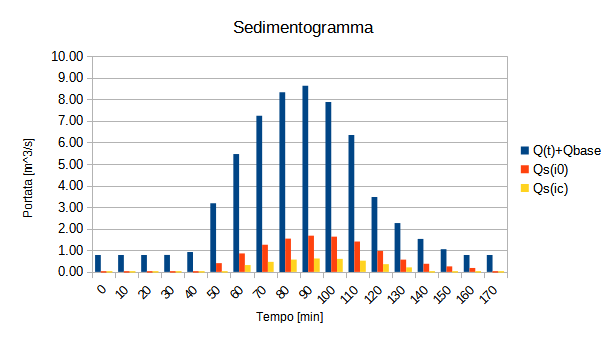
\includegraphics[scale=0.75]{immagini/sedimentogramma.png}
    \caption{Sedimentogramma del tratto di studio, per un evento di deflusso con tempo di ritorno pari a 200 anni, calcolato mediante il metodo cinematico.}
    \label{sedimentogramma}
\end{figure}

\subsection{Calcolo del trasporto solido mediante Smart-Jaeggi}
Un ulteriore metodo per il calcolo del trasporto solido di fondo avviene mediante la formula di Smart e Jaeggy (1983), che è:
\begin{equation}
    q_s = 4 \cdot \left(\frac{D_{90}}{D_{30}}\right)^{0.2} \cdot \frac{1}{\frac{\rho_s}{\rho} -1} \cdot q \cdot S^{1.6} \cdot \left( 1 - \frac{\tau_c}{\tau}\right)
\end{equation}
Nell'equazione:
\begin{itemize}
    \item $q$ e $q_s$ indicano rispettivamente le portate unitarie liquide e solide;
    \item $\tau$ e $\tau_s$ sono rispettivamente gli sforzi medi e critici dell'acqua in movimento nel corso;
    \item $\rho$ e $\rho_s$ indicano rispettivamente i valori di peso volumetrico dell'acqua e di peso volumetrico dei sedimenti dell'alveo.
\end{itemize}
Essendo che la relazione tra la portata volumetrica e lo sforzo tangenziale non è lineare, occorre ricavare la funzione interpolatrice di tali punti. Tale funzione ha come formula $\tau = \alpha \cdot Q^{\beta}$.\\
Per fare ciò, occorre creare una grafico a doppia entrata dei valori di portata e sforzo tangenziale, in condizioni di diverse profondità di tiranti idraulici.\\
Successivamente, dalla curva interpolatrice del grafico ci si ricava la tensione tangenziale reale, in funzione della portata liquida, come indicato nella formula precedentemente esposta.\\
Infine, dal valore della tensione agente sul fondo si termina lo studio del trasporto solido mediante il calcolo della portata solida e del relativo volume di sedimenti.\\
\begin{figure}[H] \centering
    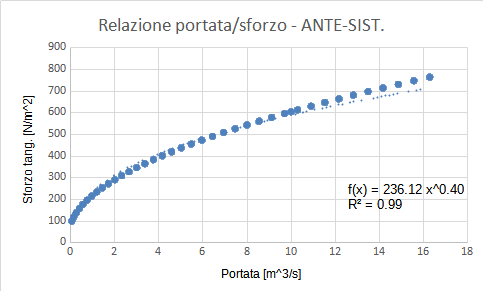
\includegraphics[scale=0.75]{immagini/rel_port_sforzo_ante_sist.png}
    \caption{Relazione tra lo sforzo tangenziale agente sulla sezione dell'alveo e la portata liquida, per un evento di piena con tempo di ritorno pari a 200 anni, ed in condizioni precedenti alla sistemazione idraulica.}
    \label{rel_port_sforzo_ante_sist}
\end{figure}
\begin{figure}[H] \centering
    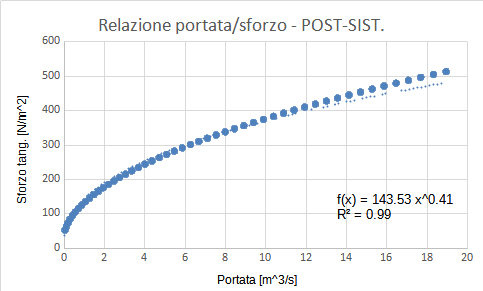
\includegraphics[scale=0.75]{immagini/rel_port_sforzo_post_sist.png}
    \caption{Relazione tra lo sforzo tangenziale agente sulla sezione dell'alveo e la portata liquida, per un evento di piena con tempo di ritorno pari a 200 anni, ed in condizioni successive alla sistemazione idraulica.}
    \label{rel_port_sforzo_post_sist}
\end{figure}


\begin{table}[H] \centering
    \caption{\textcolor{red}{Portata e volume di materiale solido, nel caso di una piena con tempo di ritorno pari a 200 anni, nella condizione precedente e successiva alla sistemazione idraulica, calcolata secondo il metodo Smart-Jaeggy.}}
    \begin{tabular}{ccccccc}
\toprule
& \multicolumn{3}{c}{Sit. ANTE SISTEM.} & \multicolumn{3}{r}{Sit. POST SISTEM.} \\
\midrule
    tempo & $\tau(i_o)$ & $Q_s(i_o)$ & $V_s(i_o)$ & $\tau(i_c)$ & $Q_s(i_c)$ & $V_s(i_c)$ \\
    (minuti) & ($N/m^2$) & $(m^3/s)$ & $(m^3)$ & $N/m^2$ & $(m^3/s)$ & $(m^3)$ \\
\midrule
    0 & 0.00 & 0.00   & 0.00 & 0.00     & 0.00   & 0.00   \\
    10 & 214.33 & 0.12   & 74.75 & 129.82      & 0.02   & 14.85  \\
    20 & 214.33 & 0.12   & 74.75   & 129.82 & 0.02   & 14.85  \\
    30       & 214.39 & 0.12   & 74.80   & 129.86 & 0.02   & 14.86  \\
    40       & 221.55  & 0.14   & 83.13   & 134.36 & 0.03   & 17.32  \\
    50       & 313.88                       & 0.40   & 239.46  & 192.81                       & 0.11   & 66.46  \\
    60       & 422.03                       & 0.93   & 556.06  & 262.08                       & 0.29   & 171.88 \\
    70       & 491.74                       & 1.41   & 848.31  & 307.09                       & 0.45   & 271.68 \\
    80       & 533.08                       & 1.76   & 1057.46 & 333.90                       & 0.57   & 343.87 \\
    90       & 551.38                       & 1.93   & 1158.96 & 345.79                       & 0.63   & 379.06 \\
    100      & 545.41                       & 1.88   & 1125.23 & 341.90                       & 0.61   & 367.35 \\
    110      & 514.08                       & 1.60   & 957.89  & 321.56                       & 0.52   & 309.44 \\
    120      & 443.73                       & 1.07   & 639.21  & 276.07                       & 0.33   & 200.11 \\
    130      & 358.51                       & 0.59   & 351.22  & 221.30                       & 0.17   & 103.16 \\
    140      & 304.26                       & 0.36   & 218.62  & 186.68                       & 0.10   & 59.72  \\
    150      & 261.17                       & 0.23   & 138.64  & 159.35                       & 0.06   & 34.29  \\
    160      & 228.18                       & 0.15   & 91.29   & 138.53                       & 0.03   & 19.76  \\
    170      & 214.33                       & 0.12   & 74.75   & 129.82                       & 0.02   & 14.85 \\
    \bottomrule
    \end{tabular}
    \end{table}
La portata solida totale trasporta precedentemente alla realizzazione dell'opera è pari a 7764.51 $m^3$, mentre per quella successiva alla sistemazione idraulica è di 2403.49 $m^3$.\\
Essendo la portata liquida totale pari a 36100.60 $m^3$, la concentrazione solida antecedente al miglioramento idraulico è di 17.70\%, mentre per quella successiva è di 6.24\%. La riduzione del trasporto solido, in presenza o in assenza delle briglie, è del 64.74\%.\\
\begin{figure}[H] \centering
    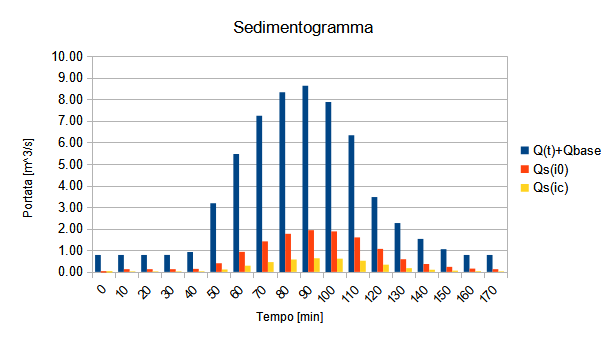
\includegraphics[scale=0.75]{immagini/sedimentogramma_smart_jaeggy.png}
    \caption{Sedimentogramma dell'evento di piena, per tempo di ritorno pari a 200 anni, calcolata mediante il metodo di Smart e Jaeggy.}
    \label{sedimentogramma_smart_jaeggy}
\end{figure}



\section{Progettazione di un'opera di consolidamento tipo}
Per iniziare il dimensionamento delle singole opere di consolidamento, occorre determinare il numero complessivo degli elementi da ereggere.\\
Opere troppo elevate generano un impatto significativo sull'ambiente, poiché tendono a deturpare il paesaggio e la risalita della fauna ittica. Opere di dimensioni troppo ridotte comportano un numero eccessivo di elementi, posti a distanza molto ravvicinata.\\
L'esperienza del professore ci consiglia di imporre un numero di briglie pari a 9, con altezza di 2.63 m.\\
I calcoli verranno svolti basandosi sul diagramma di deflussi per precipitazioni con intensità a blocchi alternati (mediante metodo cinematico), comprendenti anche il trasporto solido, per tempi di ritorno pari a 200 anni. Tale valore di portata totale è di 9.25 $m^3/s$.\\
I parametri caratteristici del tratto di torrente da sottoporre a sistemazione sono presenti nel tabella riportata precedentemente \ref{inf_morf_coll_princ}.\\
Per quanto riguarda i parametri relativi al numero di briglie, si fa riferimento al grafico precedente \ref{opzioni_numero_altezza_briglie}.
\subsection{Gaveta a profilo trapezoidale}

\subsubsection{Dimensionamento iniziale}
Si impone come larghezza inferiore della gaveta la metà della larghezza del torrente, ovvero 4 metri.\\
Successivamente ad essersi calcolati la larghezza inferiore, occorre calcolare la profondità del flusso d'acqua passante per la sezione della gaveta. Come valore di prima approssimazione si applica la formula:
\begin{equation}
    h = 0.7 \cdot q ^{2/3}
\end{equation}
Nel nostro caso, la formula diventa:
\begin{equation}
    h = 0.7 \cdot \left( \frac{9.25}{4} \right)^{2/3}
\end{equation}
Che restituisce il risultato di 1.22 m.\\
Successivamente ad aver stimato la profondità di massima, occorre ricavare la profondità corretta, utilizzando in modo iterativo la formula di Belangér (ricavandosi la medesima portata di progetto). Tale formula è la seguente:
\begin{equation}
Q = 1.705 \cdot h^{3/2} \left[L + \frac{2}{5}\cdot h \cdot \left(\frac{1}{\tan{\alpha}} + \frac{1}{\tan{\beta}}\right) \right]
\end{equation}
Si è scelto di imporre i valori $\alpha$ e $\beta$ (ovvero la pendenza delle ali laterali), pari a 60$^\circ$.\\
Dopo diversi tentativi, l'altezza che genera una portata totale di 9.25 $m^3/s$, in funzione della geometria della gaveta, è di 1.13 m.\\
Si è scelto di imporre un franco idraulico di 13 cm, in modo da portare l'altezza della sezione della gaveta a 1.30 m.\\
Avendo calcolato l'altezza della sezione trapezoidale e conoscendo la pendenza delle ali, è possibile calcolare la larghezza superiore della gaveta:
\begin{equation}
    L_{gav.sup} = L_{gav.inf} + 2 \cdot \frac{h}{\tan \alpha} 
\end{equation}
I calcoli reali portano ad una larghezza superiore della briglia di 5.50 m, essendo che la larghezza di una singola ala è di 1.25 m.\\
La larghezza media della sezione trapezoidale della briglia avviene calcolando la media tra la larghezza inferiore e superiore, che in questo caso è 4.75 m.\\
Lo spessore del coronamento della briglia (s) viene stimato utilizzando tre metodi diversi:
\begin{itemize}
    \item metodo di Zoli: $0.7 + 0.1 \cdot Z$ $\rightarrow$ 0.96 m;
    \item verifica allo scorrimento: $0.7 \cdot h$ $\rightarrow$ 0.91 m;
    \item metodo di Romiti: $0.8 + 2 \cdot D_{84}$ $\rightarrow$ 1.23 m.
\end{itemize}
Essendo che i tre risultati non si discostano molto tra di loro, viene scelto il valore più cautelativo, imponendo la larghezza del coronamento pari a 1.2 m.\\
Il dimensionamento della base del corpo briglia può avvenire applicando due formule empiriche:
\begin{itemize}
    \item metodo di Zoli: implica l'utilizzo del specifico grafico a doppia entrata $\rightarrow$ 1.80 m;
    \item metodo di Romiti: $z \sqrt{\frac{z+3 \cdot h-s^2/z}{z+h+4.55}}$ $\rightarrow$ 2.13 m.
\end{itemize}
Anche per questo caso, essendo che i valori ricavati non si discostano molto tra di loro, si scegliere di porsi nelle condizioni maggiormente cautelative, andando ad imporre una larghezza di base del corpo briglia di 2.10 m.\\
La profondità della fondamenta $(z_f)$ della briglia viene calcolata in funzione della pool erosiva che si genera a valle dell'opera (l'argomento verrà ripreso nel capitolo successivo inerente alla controbriglia), o in funzione della sola portata totale passante per la gaveta. Tale profondità può essere calcolata mediante due formule:
\begin{itemize}
    \item $z_f > 0.6 \cdot t$ $\rightarrow$ 0.63 m;
    \item $z_f > 0.15 \cdot (z+h)$ $\rightarrow$ 0.56 m
\end{itemize}
Viene scelto il valore maggiore tra i due, arrotondando a 0.65 m, per motivi pratici e di sicurezza.\\
Infine, l'ultima geometria da calcolare per quanto riguarda la briglia è inerente alla lunghezza degli sporti, sia di monte che di valle. Tale valore dev'essere minore (o uguale) a $0.7 \cdot z_f$. In questo caso, la lunghezza massima dello sporto della fondamenta è 0.45 m, ed in questo caso si impone lo stesso valore per la progettazione.\\
E' possibile che lo sporto di valle e di monte non abbiano la stessa lunghezza. 

\subsubsection{Verifiche tradizionali della briglia}
Come verrà riportato in seguito, nella sezione delle verifiche secondo NTC-2018, sono state riportate le misure della struttura già corrette e migliorate, in modo che la valutazione portasse direttamente esito positivo.\\
Prima di iniziare le verifiche dimensionali tradizionali della briglia, risulta utile riportare le misure calcolate durante il dimensionamento di massima ed i coefficienti necessari da attribuire alle forze e momenti.
\begin{table}[H] \centering
    \caption{\textcolor{red}{Valori dimensionali e coefficienti fisici necessari per effettuare la procedura di verifica della geometria della briglia.}}
    \begin{tabular}{cc}
    \toprule
    DATI                          &       \\
    \midrule
    peso sp. acqua ($N/m^3$)         & 10000 \\
    peso sp. mat. ($N/m^3$)          & 24000 \\
    altezza gaveta: h (m)         & 1.130 \\
    altezza corpo: z(m)           & 2.63  \\
    coronamento: s (m)            & 1.20  \\
    base corpo: b (m)              & 2.10  \\
    base fondazione: Bf (m)       & 2.40  \\
    altezza fondazione: zf (m)    & 0.65  \\
    sporto monte:sm (m)            & 0.30  \\
    sporto valle: sv (m)           & 0.00  \\
    coeff. attrito: fmur           & 0.7   \\
    coeff. attrito terreno: fterr & 0.45  \\
    coeff. riduz.sottospinta.: m  & 0.20  \\
    \bottomrule
    \end{tabular}
\end{table}
Inoltre, risulta necessario riportare le caratteristiche del terreno su cui l'opera poggia.
\begin{table}[H] \centering
    \caption{\textcolor{red}{Caratteristiche fisiche del terreno del tratto da sistemare, necessarie per poter iniziare la verifica sulla briglia.}}
    \begin{tabular}{cc}
    \toprule
    angolo di attrito & 36.0      \\
    2/3 ang. attrito  & 24.0      \\
    tangente          & 0.45      \\
    cap.portante      & 0.35 MPa \\
    \bottomrule
    \end{tabular}
    \end{table}

Dopo aver esposto le geometrie ed i coefficienti essenziali per la verifica, è necessario riportare quali sono le forze ed i momenti agenti/reagenti sul profilo della briglia.
\begin{figure}[H]  \centering
    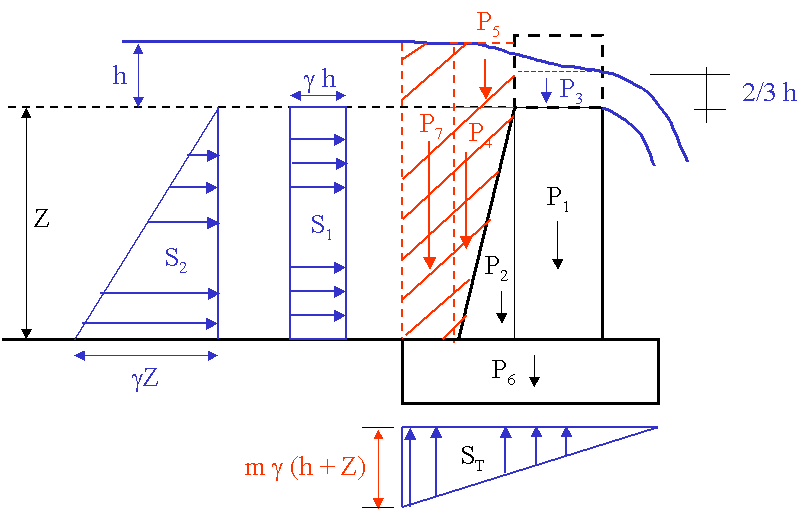
\includegraphics[scale=0.5]{immagini/forze_agenti_briglia.png}
    \caption{Rappresentazione delle forze e dei momenti agenti e reagenti sul profilo della briglia.}
    \label{forze_agenti_briglia}
\end{figure}

\begin{table}[H] \centering
    \caption{\textcolor{red}{Valori relativi alla verifica tradizionale del solo corpo briglia. La sottospinta idraulica viene trascurata, poiché riguarda la fondazione dell'opera.}}
    \begin{tabular}{ccccc}
    \toprule
           & Forze (N) & bracci (m) & Momenti (N m)    &         \\
    \midrule
    P1 (N) & 75744     & 0.60       & 45446.4          &         \\
    P2 (N) & 28404     & 1.50       & 42606            &         \\
    P3 (N) & 9040      & 0.60       & 5424             &         \\
    P4 (N) & 11835     & 1.80       & 21303            &         \\
    P5 (N) & 10170     & 1.65       & 16780.5          &         \\
    somma  & 135193.0  &            & 131559.9         & stab.   \\
    \midrule
    S1 (N) & 29719     & 1.32       & 39080.5        &         \\
    S2 (N) & 34584.5   & 0.88       & 30319.1 &         \\
    somma  & 64303.5   &            & 69399.6          & destab. \\
    \bottomrule
    \end{tabular}
    \end{table}

    \begin{table}[H] \centering
        \caption{\textcolor{red}{Valori relativi alla verifica tradizionale del corpo briglia e della fondazione. In questo caso la sottospinta idraulica viene considerata.}}
        \begin{tabular}{ccccc}
            \toprule
           & Forze (N) & bracci (m) & Momenti (N m)    &         \\
    \midrule
        P1 (N)        & 75744    & 0.60 & 45446.4          &         \\
        P2 (N)        & 28404    & 1.50 & 42606            &         \\
        P3 (N)        & 9040     & 0.60 & 5424             &         \\
        P4 (N)        & 11835    & 1.80 & 21303            &         \\
        P5 (N)        & 10170    & 1.65 & 16780.5          &         \\
        P6 (N)        & 37440    & 1.20 & 44928            &         \\
        P7 (N)        & 11280    & 2.25 & 25380            &         \\
        ST (N) (neg.) & 9024     &      &                  &         \\
        somma         & 174889.0 &      & 201867.9         & stab.   \\
       \midrule
        S1 (N)        & 29719    & 1.97 & 58397.8          &         \\
        S2 (N)        & 34584.5  & 1.53 & 52799.0          &         \\
        ST (N)        &          & 1.60 & 14438            &         \\
        somma         & 64303.5  &      & 125635.2         & destab. \\
        \bottomrule
        \end{tabular}
        \end{table}

Avendo calcolato i valori delle spinte e dei momenti agenti nel sistema, è possibile riportare i risultati della verifica allo scorrimento ed al ribaltamento.
\begin{table}[H] \centering
    \caption{\textcolor{red}{Risultati della verifica a scorrimento e ribaltamento del corpo briglia e del corpo briglia con la fondazione.}}
    \begin{tabular}{cc}
    \toprule
    \multicolumn{2}{c}{CORPO BRIGLIA} \\
    $G_{scorr}$                               & 1.47                 \\
    $G_{rib}$                              & 1.90                 \\
    u (m)                             & 0.460                \\
    e (m)                             & 0.590                \\
    b/3 (m)                           & 0.700                \\
    sigma valle (MPa)                 & 0.173                \\
    sigma monte (MPa)                 & -0.044               \\
    \midrule
    \multicolumn{2}{c}{CORPO+FONDAZIONE}                     \\
    $G_{scorr}$                       & 1.21                 \\
    $G_{rib}$                         & 1.61                 \\
    u (m)                             & 0.436                \\
    e (m)                             & 0.764                \\
    b/3 (m)                           & 0.800                \\
    sezione reagente (m)              & 1.3                  \\
    sigma valle (MPa)                 & 0.267                \\
    sigma monte (MPa)                 & 0.000                \\
    \bottomrule
    \end{tabular}
    \end{table}

La verifica allo scorrimento, secondo il metodo tradizionale, è guidata dalla formula $\Sigma F_{orizz.}<f\cdot\Sigma F_{vert.}$, dove $f$ è il coefficiente di attrito corpo-fondazione o tra la fondazione ed il terreno.\\
Con questa verifica si valuta la tendenza alla traslazione effettuata dalle forze orizzontali agenti sul sistema.\\
Portando la sommatoria delle forze verticali a destra della disequazione, risulta che la verifica è accettata se il rapporto tra le forze (comprendente il coefficiente d'attrito) è superiore a 1. In entrambi i casi, la verifica allo scorrimento risulta soddisfatta.\\
Per quanto riguarda la verifica al ribaltamento, secondo il metodo tradizionale, la formula generale è $G_s = \frac{\Sigma M_{O,stab.}}{\Sigma M_{O,rib.}} \ge 1.5$.\\
Anche per questa verifica, in entrambi i casi la struttura viene considerata sicura.\\
Infine, per quanto riguarda lo schiacciamento, che si manifesta tra corpo briglia e fondazione, e tra la fondazione ed il terreno, la formula generale è $\sigma= \frac{\Sigma F_v}{B} \cdot \left(1 \pm \frac{6 \cdot e}{B}\right)$. Tale tensione calcolata ($\sigma$) dev'essere inferiore rispetto a quella sopportabile dal materiale con cui è fatta l'opera; mentre la tensione ammissibile dal calcestruzzo è 0.35 MPa, quella agente sull'opera è di 0.267 MPa.

\subsubsection{Verifiche NTC-2018 della briglia}
Come anticipato nelle verifiche precedenti, in questa sezione verranno riportati solamente i valori geometrici accettabili secondo la verifica NTC-2018 (Norme Tecniche Costruzione).\\
Tale metodo implica l'utilizzo di coefficienti tabellati, in modo da incrementare l'effetto delle forze destabilizzanti e di ridurre l'effetto stabilizzante sull'opera. Ogni tabella ha un codice proprio, e per ogni caso di studio è frequente trovare una serie di codici, poiché avviene la combinazione dei diversi coefficienti.\\
Si comincia la verifica riportando i valori geometrici (finali e corretti) necessari per svolgere la verifica al ribaltamento della struttura.
\begin{table}[H] \centering
    \caption{\textcolor{red}{Valori dimensionali e coefficienti fisici necessari per effettuare la procedura di verifica al ribaltamento della briglia secondo NTC-2018. Tali valori sono differenti rispetto a quelli di massima stimati inizialmente.}}
    \begin{tabular}{cc}
    \toprule    
        DATI & \\
    \bottomrule
    peso sp. acqua ($N/m^3$)      & 10000 \\
    peso sp. mat. ($N/m^3$)       & 24000 \\
    altezza gaveta: h (m)      & 1.13  \\
    altezza corpo: z(m)        & 2.63  \\
    coronamento: s (m)         & 1.20  \\
    base corpo: b(m)           & 2.30  \\
    base fondazione: $B_f$ (m)    & 2.75  \\
    altezza fondazione: $z_f$ (m) & 0.90  \\
    sporto monte: $s_m$(m)         & 0.45  \\
    sporto valle: $s_v$(m)        & 0.00  \\
    coeff. riduz.sottosp.: m   & 0.20  \\
    \bottomrule
    \label{valori_dimensionali_NTC2018}
    \end{tabular}
\end{table}
La verifica al ribaltamento, secondo i criteri A1, M1 e R3, genera i seguenti risultati.
\begin{table}[H] \centering
    \caption{\textcolor{red}{Valori dei coefficienti, delle forze e dei momenti, necessari per svolgere la verifica al ribaltamento della struttura, secondo le NTC-2018 e criteri A1, M1 e R3.}}
    \begin{tabular}{cccccl}
\toprule
& Coeff. parz. & Forze (N) & bracci (m) & Momenti (N m) &  \\
\midrule
P1 (N) & 0.9                & 68169.6   & 0.60       & 40902 &   \\
P2 (N) & 0.9    & 31244.4   & 1.57       & 48950            &         \\
P3 (N) & 0.9     & 8136      & 0.60       & 4882             &         \\
P4 (N) & 0.9     & 13018.5   & 1.93       & 25169            &         \\
P5 (N) & 0.9         & 11187     & 1.75       & 19577            & \\
P6 (N)       & 0.9   & 53460     & 1.38       & 73508        &         \\
P7 (N) & 0.9       & 15228     & 2.53       & 38451            & \\
ST (N) sottosp. & sfav.		1.5  & 15510     & &  & \\
somma                  &      & 184933.5  &  & 251437.5    & stab.   \\
\midrule
& Coeff. parz. &  &            &    &         \\
S1 (N)      & 1.1                & 32690.9   & 2.22   & 72410.34  & \\
S2 (N) & 1.1     & 38042.9  & 1.78       & 67589.64 &         \\
ST (N) sottosp.        &  &   & 1.83       & 28435            &         \\
somma  &      & 70733.9   &            & 168435.0         & destab. \\
\bottomrule
    \end{tabular}
    \end{table}
Affinché la verifica possa essere considerata accettata, è necessario che il momento reagente (compreso del fattore di correzione) sia superiore rispetto a quello agente.\\
Infatti, per un momento stabilizzante (compreso del coefficiente idoneo) di 218.6 kNm, il momento agente è di 168.4 kNm, per cui la verifica al ribaltamento è soddisfatta.

Successivamente alla verifica al ribaltamento secondo la NTC-2018, è necessario verificare la struttura (corpo e fondazione) alla forza di scorrimento agente.\\
I valori dimensionali con cui è svolta la verifica allo scorrimento sono i medesimi della verifica al ribaltamento secondo la NTC-2018 (riportati nella tabella \ref{valori_dimensionali_NTC2018}).\\
Come per la verifica al ribaltamento, anche quella allo scorrimento viene svolta secondo i coefficienti dei criteri A1, M1 e R3; tali valori generano i seguenti risultati.

\begin{table}[H] \centering
    \caption{\textcolor{red}{Valori dei coefficienti, delle forze e dei momenti, necessari per svolgere la verifica allo scorrimento della struttura (corpo e fondazione), secondo le NTC-2018 e criteri A1, M1 e R3.}}
    \begin{tabular}{cccccl}
\toprule
& Coeff. parz. & Forze (N) & bracci (m) & Momenti (N m) &         \\
\midrule
    P1 (N) & 1.0  & 75744              & 0.60       & 45446 &         \\
    P2 (N) & 1.0  & 34716 & 1.57       & 54388         &         \\
    P3 (N)        & 1.0    & 9040               & 0.60       & 5424 &\\
    P4 (N)        & 1.0 & 14465 & 1.93  & 27966                  & \\
    P5 (N)        & 1.0                & 12430 & 1.75 & 21753    & \\
    P6 (N)        & 1.0   & 59400              & 1.38       & 81675  & \\
    P7 (N)        & 1.0 & 16920 & 2.53       & 42723         & \\
    ST (N) (neg.) & 1.5                & 15510  & -          & -   & \\
    somma         &        & 207205.0   &  & 279375.0  & stab. \\
    \midrule
    & Coeff. parz. & &   &                        &         \\
    S1 (N)        & 1.3 & 38634.7 & 2.22 & 85576                  & \\
    S2 (N)        & 1.3 & 44959.85 & 1.78       & 79879     &         \\
       &       &   & &      &         \\
    somma & & 83594.55  &    & 165454.5               & destab. \\
    \bottomrule
    \end{tabular}
    \end{table}

Affinché la struttura possa essere considerata verificata allo scorrimento, occorre che la componente resistiva della forza sia superiore rispetto a quella agente massima.\\
In questo caso, la componente orizzontale resistente è di 83.9 kN, mentre quella agente è di 83.6 kN; ne consegue che l'opera è dimensionata correttamente a scorrimento.\\

Al fine di analizzare la resistenza totale della struttura secondo le NTC-2018, è necessario valutare il carico limite resistivo.\\
Come per gli altri casi, la sezione di studio è quella tra il corpo della briglia e della fondazione.

\begin{table}[H] \centering
\caption{\textcolor{red}{Valori dei coefficienti, delle forze e dei momenti, necessari per svolgere la verifica al carico limite della struttura (corpo e fondazione), secondo le NTC-2018 e criteri A1, M1 e R3.}}
    \begin{tabular}{cccccl}
\toprule
& Coeff. & Forze (N) & bracci (m) & Momenti (N m) &         \\
\midrule
P1 (N) & 1.0         & 75744     & 0.60       & 45446         &         \\
P2 (N) & 1.0         & 34716     & 1.57       & 54388         &         \\
P3 (N) & 1.0         & 9040      & 0.60       & 5424          &         \\
P4 (N) & 1.0         & 14465     & 1.93       & 27966         &         \\
P5 (N) & 1.0         & 12430     & 1.75       & 21753         &         \\
P6 (N) & 1.0         & 59400     & 1.38       & 81675         &         \\
P7 (N) & 1.0         & 16920     & 2.53       & 42723         &         \\
ST (N) (neg.) & 0.0  & 0.0       & -          & -             &         \\
somma         &      & 222715.0  &            & 279375.0      & stab.   \\
\midrule
& Coeff. &     &            &               &         \\
S1 (N)        & 1.3  & 38634.7   & 2.22       & 85576         &         \\
S2 (N)        & 1.3  & 44959.85  & 1.78       & 79879         &         \\
somma         &      & 83594.6   &            & 165454.5      & destab. \\
\bottomrule
    \end{tabular}
    \end{table}

Come per gli altri casi, affinchè la struttura possa essere considerata resistente alla sollecitazione della verifica, la componente destabilizzante dev'essere inferiore alla componente stabilizzante. In questo caso, la reazione resistente del terreno è pari a 225.8 $kN/m$, mentre la tensione reale verticale che si genera è di 222.7 $kN/m$; ciò implica che la verifica al carico limite è positiva.
\section{Dimensionamento della controbriglia a valle della briglia cardine}
\section{Disegno in scala dell'opera progettata}
I disegni tecnici, allegati nelle successive pagine, rappresentano sia le singole opere (briglia e controbriglia) e sia la sistemazione complessiva del tratto di torrente.\\
Al fine di rendere l'opera meno impattante dal punto di vista paesaggistico, e maggiormente realistica, è stato ipotizzato che la superficie dell'opera abbia un rivestimento esterno in pietra a faccia vista.\\
Essendo che in fase di dimensionamento le due ali laterali sono state ipotizzate orizzontali, di conseguenza il disegno tecnico deve rappresentare allo stesso modo le sezioni dell'opera.\\
Generalmente però, le ali della briglia hanno una pendenza all'incirca del 10\% rispetto all'orizzontale, in modo da permettere il passaggio di portate con tempi di ritorno superiori a quello di progetto. In tale modo, si scongiura anche il rischio di eventuali aggiramenti del torrente rispetto alla briglia di consolidamento.

\includepdf[pages=-]{disegno_briglia.pdf}
\includepdf[pages=-]{disegno_sistemazione.pdf}
%\section{Descrizione del bacino e nozioni teoriche}

\subsection{Il fiume Boite ed il suo bacino}
Il fiume Boite è un corso idrico a carattere torrentizio delle Dolomiti. Le sue caratteristiche principali sono le seguenti:
\begin{itemize}
    \item lunghezza: 45.07 km;
    \item portata media: 12.71 $\frac{m^3}{s}$;
    \item area del bacino idrografico: 395.9 km$^2$;
    \item altitudine della sorgente: 1800 m s.l.m.;
\end{itemize}
Tale corso idrico è alimentato da diversi affluenti, e sfocia nel fiume Piave.
\cite{fiume_boite}
\subsection{La briglia filtrante}
Una briglia filtrante è una struttura antropica che viene posta lungo i corsi d'acqua montani.\\
L'obiettivo di tali opere è quello di consentire il passaggio dell'acqua del corso idrico, e di selezionare la quantità di sedimenti in movimento.\\
Per fare ciò, tali briglie possiedono:
\begin{itemize}
    \item una o più aperture nel corpo centrale;
    \item una "piazza di deposito" a monte, dove avviene il deposito dei detriti.
\end{itemize} 
Il ridotto passaggio di acqua attraverso le aperture (durante un evento di piena) riduce la velocità di flusso; ne deriva una minore capacità di trasporto di detriti, i quali vengono depositati.
\cite{prov_bolz}\\
Successivamente al picco di piena, la velocità di passaggio dell'acqua aumenta nuovamente, permettendo lo svuotamento dai detriti della "piazza di deposito".

\subsection{Linea segnalatrice di probabilità pluviometrica}
La linea segnalatrice di probabilità pluviometrica è un parametro matematico che riguarda gli eventi di precipitazione.\\
Tale funzione mette in relazione la quantità massima di evento pluviometrico, la sua durata ed il suo tempo di ritorno. \\
La LSPP si ricava andando ad elaborare i dati storici di precipitazione accaduti in un particolare territorio: la curva risultante sarà caratteristica di quel dato luogo.\\
La procedura di calcolo della LSPP si articola in diversi passaggi. \\
Come primo passaggio occorre andare ad ordinare i valori storici di precipitazione, in ordine crescente. Dopo aver fatto ciò, si assegna ad ogni valore la propria plotting position, attraverso la formula di Weibull:
\begin{equation}
\label{P_em}
    P_{em}=\frac{i}{N+1}
\end{equation}
Tale formula permette di valutare la probabilità di non superamento di un fenomeno, solamente valutando la sua disposizione in una serie di dati.\\
Successivamente, dai dati storici di precipitazione si ricavano i parametri statistici di media e deviazione standard, rispettivamente secondo le successive formule:
\begin{equation}
\label{media_aritmetica}
    m = \frac{x_1+x_2+...+x_N}{N}
\end{equation}
\begin{equation}
\label{dev.st}
    \sigma = \sqrt{\frac{\Sigma(X_1 - \mu)^2}{N+1}}
\end{equation}
Da questi due valori statistici si calcolano i parametri della distribuzione F(y), ovvero $\alpha$ e $u$, mediante il metodo dei momenti:
\begin{equation}
\label{alpha}
\alpha = \frac{\sqrt{6} \cdot \sigma}{\pi}    
\end{equation}
\begin{equation}
\label{u}
    u = \bar{h} - 0.5772 \cdot \alpha
\end{equation}
Conoscendo questi parametri è possibile ricavare la variabile ridotta $y = \frac{\bar{h}-u}{\alpha}$, che permette finalmente di trarre la funzione della distribuzione di Gumbel:
\begin{equation}
  F(y) = e^{e^{-y}}
\end{equation}
E' possibile creare un grafico che metta in relazione l'altezza di precipitazione h (in ordinata) e la relativa variabile ridotta ricavata dai calcoli (in ascissa): facendo ciò si adatta la distribuzione di probabilità di Gumbel.

Il programma con cui è stato ricavato questo grafico (Excel) permette di conoscere la funzione della linea di tendenza, e del relativo valore di $R^2$. \\
Il valore $R^2$, anche detto "Coefficiente di determinazione" è un parametro statistico che permette di misurare il legame tra la variabilità dei dati e la correttezza del modello statistico utilizzato. \cite{r_quadro} \\
Successivamente, è possibile procedere al confronto grafico tra la probabilità empirica P di Weibull e la F(h):

La disposizione dei punti attorno la bisettrice permette di intuire come i valori di probabilità siano congruenti reciprocamente.\\
Un altro indicatore con cui è possibile valutare la concordanza di probabilità è il $\chi ^2$. Infatti, tale parametro statistico permette di verificare se le frequenze dei valori osservati si adattano a quelle teoriche, di una distribuzione di probabilità prefissata.\\
Al fine di confermare la coerenza tra le probabilità, il valore del $\chi ^2$ calcolato dev'essere inferiore a quello teorico.\\
Per esempio, nel caso di adattabilità di 1h: 
\begin{itemize}
    \item $\chi ^2$ calcolato: 3.9375
    \item $\chi ^2$ teorico: 5.9915
\end{itemize}
Al fine di conoscere la precipitazione prevista ($h_t$) per un certo tempo di ritorno, occorre valutare la relativa linea segnalatrice di possibilità pluviometrica.\\
Per fare ciò, si utilizzerà la formula 
\begin{equation}
    y_{t}= -\ln \left[ \ln \left(\frac{1}{F(h)} \right) \right] \rightarrow y_{t}= -\ln \left[ \ln \left(\frac{T}{T-1} \right) \right]
    \label{variabile_ridotta}
\end{equation}
Dopo aver trovato il parametro $y_t$, si andrà a ricavare $h_t$ mediante la successiva formula:
\begin{equation}
h_t = u + \alpha \cdot y_t    
\label{h_t}
\end{equation}
Questi calcoli potranno essere ripetuti per ogni fascia oraria disponibile e per qualsiasi tempo di ritorno.\\
Per esempio, la linea segnalatrice di possibilità pluviometrica del nostro bacino, per un tempo di ritorno di 10 anni, è la seguente.

Anche per questo caso, il programma che ha permesso il calcolo permette di inserire la funzione matematica della linea di tendenza, che in questo caso è $h_{10}= 31.9547 \cdot x^{0.3537}$. \\
Da tale espressione è possibile conoscere l'altezza di precipitazione di qualsiasi durata (possibilmente inferiore alle 24 ore), per tempo di ritorno di 10 anni. Infatti, nella formula l'incognita è rappresentata dal tempo di durata dell'evento di pioggia.

\subsection{Calcolo della portata di picco}
Lo studio della portata di picco è essenziale per conoscere la massima quantità d'acqua in movimento nel bacino, soprattutto nel caso in cui la durata di un evento pluviometrico eguagli il tempo di corrivazione del bacino.\\
Infatti, è proprio questa la peggiore condizione idraulica, poichè:
\begin{itemize}
    \item all'aumentare della durata di precipitazione l'intensità non aumenta in modo direttamente proporzionale;
    \item al diminuire della durata di precipitazione l'altezza di pioggia è direttamente proporzionale.
\end{itemize}
La funzione che permette di conoscere la portata di picco ($Q_p$) è la seguente:
\begin{equation}
    Q_p = C_d \cdot \frac{h_r \cdot A}{t_c}
    \label{Qp}
\end{equation}
dove: 
\begin{itemize}
    \item $C_d$ è il coefficiente di deflusso;
    \item $h_r(t_c, T_r)$ è l'altezza di pioggia corrispondente al tempo di corrivazione $t_c$ ed al tempo di ritorno $T_r \rightarrow h_r = a \cdot t_c ^n$;
    \item $A$ è l'area del bacino.
\end{itemize}
\subsubsection*{Il tempo di corrivazione}
Il tempo di corrivazione di un bacino ($t_c$) è il tempo massimo che impiega una goccia per attraversare completamente il bacino, fino ad arrivare alla sezione di chiusura.\\
Tale tempo di passaggio può essere calcolato in diversi modo, per questa relazione è stata utilizzata la formula di Giandotti:
\begin{equation}
    t_c = \frac{4 \sqrt{A} + 1.5 \cdot L}{0.8 \cdot \sqrt{z}}
    \label{giandotti}
\end{equation}
dove: 
\begin{itemize}
    \item $A$ è l'area del bacino, in $km^2$;
    \item $L$ è la lunghezza dell'asta principale, in $km$;
    \item $z$ è l'altezza media del bacino rispetto alla sezione di chiusura, espressa in $m$.
\end{itemize}
\subsubsection*{Il coefficiente di deflusso}
Il coefficiente di deflusso è il rapporto tra la precipitazione efficace del bacino e la precipitazione totale. Offre in maniera generale una rappresentazione del deflusso superficiale e dell'infiltrazione del bacino.\\
La formula è quindi:
\begin{equation}
    C_d = \frac{P_e}{h_r}
    \label{Cd}
\end{equation}
\subsubsection*{La precipitazione efficace}
La precipitazione efficace equivale alla quantità d'acqua dell'evento meteorico, al netto delle perdite iniziali e dell'imbibimento del terreno. In pratica è la frazione di precipitazione che si trasforma in deflusso superficiale.\\
Tale valore varia in base alle condizioni del terreno ed in funzione delle caratteristiche del territorio.\\
La formula per calcolare la precipitazione efficace è la seguente: 
\begin{equation}
    P_e = \frac{(h_r - I_a)^2}{h_r - I_a + S}
    \label{Pe}
\end{equation}
dove la lettera $S$ indica lo storage idrico del terreno, che può essere calcolato mediante: 
\begin{equation}
    S = S_0 \cdot \left ( \frac{100}{CN} -1 \right )
    \label{storage}
\end{equation}
Nella precedente funzione, la costante $S_0$ equivale a 254 mm ed il valore CN quantifica la permeabilizzazione del suolo.

\subsection{Progetto della sezione di un canale}
Generalmente, in assenza di vincoli esterni e tecnici, durante il dimensionamento di un canale si adotta la sezione di minima resistenza, ovvero quella sezione che a parità di area permette la velocità media massima, e quindi la portata massima.\\
A parità di altre condizioni, la velocità media dipende dal valore di raggio idraulico (e quindi dalla forma e dimensione della sezione).
\subsubsection*{Calcolo della profondità di moto uniforme $y_1$}
Il parametro $y_1$ indica la profondità del canale con cui la portata $Q$ viene convogliata con la sezione di minor perimetro bagnato.\\
Il calcolo della profondità critica è un metodo iterativo, ovvero il risultato finale si ottiene dalla ripetizione di una serie di calcoli.
Il procedimento inizia con il calcolo di una profondità di primo tentativo $y_0$, mediante la seguente equazione:
\begin{equation}
    y_0 = \left ( \frac{Q}{B \cdot K_S \cdot \sqrt{i_F}} \right) ^ {\frac{3}{5}}
    \label{prof_critica_tentativo}
\end{equation} 
Successivamente si calcola il relativo raggio idraulico, mediante la formula:
\begin{equation}
    Rh_0 = \frac{B \cdot y_0}{B + 2\cdot y_0}
    \label{raggio_idraulico}
\end{equation} 
E da questo raggio idraulico si calcola nuovamente l'altezza $y$:
\begin{equation}
    y_1 = \frac{Q}{B \cdot K_S \cdot R_h ^\frac{2}{3} \cdot \sqrt{i_F}}
    \label{prof_critica}
\end{equation} 
Nel caso che la differenza percentuale tra le due profondità è inferiore al 2\%, il processo può terminare; in caso contrario, occorre ripetere i procedimenti, calcolando il raggio idraulico mediante l'ultima profondità critica ottenuta.
\begin{equation}
    \frac{|y_1 - y_0|}{y_0} \le 2\%
    \label{scostamento_prof_critica}
\end{equation} 
\subsubsection*{Calcolo della $H$ del canale}
Avendo i valori di $y_c$ (calcolata) e di $B$ (di progetto), è possibile calcolare il valore $H$, ovvero l'energia specifica del canale.
La formula per calcolare $H$ è la seguente: 
\begin{equation}
    H = y + \frac{q^2}{2 \cdot g \cdot y^2}
    \label{energia_specifica_canale}
\end{equation} 
Il parametro $q$ indica la portata del canale per unità di larghezza, e si calcola con $q = \frac{Q}{B}$.
\subsubsection*{Calcolo della larghezza limite $B_L$, per il passaggio in condizioni critiche}
Il valore $B_L$, ovvero la larghezza della sezione rettangolare della briglia, in condizioni critiche, si calcola con la seguente formula:
\begin{equation}
    B_L = \frac{Q}{0.414 \cdot \sqrt{g} \cdot H_1 ^{1.5}}
    \label{larghezza_specifica}
\end{equation}
%\section{Elaborazione dati}
I seguenti procedimenti di calcolo interessano valori valutati per un tempo di ritorno di 50 anni.\\
In questo capitolo verranno effettuati i calcoli di progetto, in concordanza con le nozioni teoriche esposte nella sezione precedente.\\
Per semplificare l'esposizione, verranno mostrati solamente i calcoli per eventi pluviometrici di 1 ora di durata. Ovviamente i calcoli sono stati ripetuti per ogni durata di evento pluviometrico (1, 3, 6, 12 e 24 ore), per il tempo di ritorno di 50 anni.
\subsection{Dati storici di precipitazione}
% Please add the following required packages to your document preamble:
% \usepackage{multirow}
\begin{table}[H] \centering \footnotesize
\begin{tabular}{cccccc}
\multirow{3}{*}{\textbf{Anno}} & \multicolumn{5}{l}{\textbf{Pioggia in mm}}                                           \\
\toprule
                               & \textbf{1 ora} & \textbf{3 ore} & \textbf{6 ore} & \textbf{12 ore} & \textbf{24 ore} \\
                               & \textbf{mm}    & \textbf{mm}    & \textbf{mm}    & \textbf{mm}     & \textbf{mm}     \\
\midrule
1992                           & 14.6           & 21             & 33.2           & 60.8            & 78              \\
1993                           & 18.4           & 23.4           & 41.8           & 65.4            & 76.6            \\
1994                           & 19.6           & 34.4           & 47.2           & 64.8            & 83.2            \\
1995                           & 15.8           & 19.6           & 32             & 41.6            & 51              \\
1996                           & 24.8           & 31             & 40             & 64.8            & 100             \\
1997                           & 28.6           & 36             & 36             & 55.6            & 69              \\
1998                           & 17.8           & 28.2           & 39             & 55.2            & 78              \\
1999                           & 11.8           & 30.2           & 48.4           & 81.4            & 96.4            \\
2000                           & 15.8           & 25.4           & 46.4           & 67.8            & 73.4            \\
2001                           & 25.4           & 46.2           & 50.6           & 61.8            & 72              \\
2002                           & 17.8           & 31.6           & 40             & 63.6            & 98.8            \\
2003                           & 21.6           & 25.4           & 41.6           & 71.6            & 91.2            \\
2004                           & 13.8           & 21             & 33.4           & 36.6            & 48.2            \\
2005                           & 26.2           & 31.4           & 37.2           & 50.4            & 69.8            \\
2006                           & 14.8           & 27.2           & 48.4           & 63.8            & 69.6            \\
2007                           & 32.2           & 43.4           & 44.8           & 50.8            & 78.2            \\
2008                           & 19             & 23.8           & 38.6           & 58.4            & 72              \\
2009                           & 20             & 25.8           & 34             & 53.6            & 95.4            \\
2010                           & 8.8            & 18.2           & 30.2           & 47              & 78.4            \\
2011                           & 25             & 27.2           & 31.4           & 49.6            & 81.8            \\
2012                           & 18.2           & 28.2           & 49.8           & 83              & 104             \\
2013                           & 16.8           & 22             & 39             & 61.8            & 69.2            \\
2014                           & 31.2           & 32.4           & 44             & 73.4            & 114.8           \\
2015                           & 20.2           & 25.4           & 36.8           & 42.8            & 50.2            \\
2016                           & 12             & 28.8           & 46.2           & 63              & 67.8            \\
2017                           & 25.4           & 29.2           & 36             & 62.6            & 72.4            \\
2018                           & 65.6           & 73             & 73.4           & 87              & 146.4           \\
2019                           & 16.6           & 24.2           & 42             & 60.4            & 85.6            \\
2020                           & 28.8           & 37.4           & 47.8           & 65.8            & 120.6           \\
2021                           & 26.2           & 37.4           & 45.6           & 51.6            & 54.6            \\
2022                           & 23.2           & 38             & 44             & 44.6            & 46.6            \\
2023                           & 34.6           & 35.4           & 52.2           & 67.4            & 96.2       \\
\bottomrule
\end{tabular}
\end{table}
\subsection{Calcolo della LSPP}
Successivamente ad aver ordinato in ordine crescente le altezze di precipitazione, si è assegnato ad ogni evento pluviometrico un indice di Weibull, mediante la formula \ref{P_em}.
Dopo aver fatto ciò, si calcolano i parametri statistici di media e deviazione standard, rispettivamente mediante le formule \ref{media_aritmetica} e \ref{dev.st}. \\

\begin{equation}
      m = \frac{x_1+x_2+...+x_N}{N} = \frac{8.8+...+65.6}{32} = 22.21 mm
\end{equation}
\begin{equation}
      \sigma = \sqrt{\frac{\Sigma(X_1 - \mu)^2}{N+1}}= \sqrt{\frac{(8.8 - 22.21)^2+...(65.6-22.21)^2}{32+1}} = 10.13 mm
\end{equation}
E da questi valori appena calcolati, ci si calcola i parametri della distribuzione F(y), utilizzando le formule \ref{alpha} e \ref{u}:
\begin{equation}
    \alpha = \frac{\sqrt{6} \cdot \sigma}{\pi} = \frac{\sqrt{6} \cdot 22.21}{\pi} = 7.90
\end{equation}
\begin{equation}
    u = \bar{h} - 0.5772 \cdot \alpha = 10.13- 0.5772 \cdot 7.90 = 17.65
\end{equation}
Successivamente, si effettua il calcolo della variabile ridotta, rispetto al tempo di ritorno, come secondo la formula \ref{variabile_ridotta}:
\begin{equation}
y_{t}= -\ln \left[ \ln \left(\frac{T}{T-1} \right) \right] = -\ln \left[\ln \left( \frac{50}{50-1} \right) \right ] = 3.902
\end{equation}
Ed infine si calcola l'altezza di precipitazione per il dato tempo di ritorno, utilizzando la formula \ref{h_t}:
\begin{equation}
h_t = u + \alpha \cdot y_t  = 17.65 + 7.90 \cdot 3.902= 48.5mm
\end{equation}
Infine, si effettua il test del $\chi^2$, che per semplicità verrà svolto dall'apposita funzione di Excel. I risultati sono i seguenti: 
\begin{itemize}
    \item $\chi ^2$ calcolato: 3.9375
    \item $\chi ^2$ teorico: 5.9915
\end{itemize}
\subsection{Calcolo della portata di picco} \label{portatadipicco}
Le caratteristiche del bacino sono le seguenti:
\begin{itemize}
    \item differenza totale di quota: 1000 m;
    \item CN: 85;
    \item area del bacino: 4 km$^2$;
    \item lunghezza dell'asta principale: 4 km;
    \item pendenza del reticolo idraulico (i$_f$): 0.025.
\end{itemize}
Utilizzando la formula di Giandotti \ref{giandotti} calcolo il tempo di corrivazione del reticolo (t$_c$):
\begin{equation}
    t_c = \frac{4 \sqrt{A} + 1.5 \cdot L}{0.8 \cdot \sqrt{z}} = \frac{4 \sqrt{4} + 1.5 \cdot 4}{0.8 \cdot \sqrt{1000}} = 0.48 h
\end{equation}
Al fine di conoscere la quantità di precipitazione efficace, per conoscere il coefficiente di deflusso, occorre quantificare lo storage idrico del suolo. Per fare ciò utilizzo la formula \ref{storage}
\begin{equation}
    S = S_0 \cdot \left ( \frac{100}{CN} -1 \right ) = 254 \cdot \left ( \frac{100}{85} - 1 \right) = 44.82mm
\end{equation}
Da questo parametro è possibile calcolare la precipitazione efficace, mediante la formula \ref{Pe}:
\begin{equation}
    P_e = \frac{(h_r - I_a)^2}{h_r - I_a + S} = \frac{(33.87 - 0.1 \cdot44.82)^2}{33.87 - 0.1\cdot48.82 + 48.82}= 11.64 mm
\end{equation}
Da questi valori è possibile calcolare il coefficiente di deflusso del bacino, mediante la formula \ref{Cd}:
\begin{equation}
    C_d = \frac{P_e}{h_r} = \frac{11.64}{33.87}= 0.36
\end{equation}
Infine, si calcola la portata di picco del reticolo idrografico del bacino, utilizzando la formula \ref{Qp}:
\begin{equation}
    Q_p = C_d \cdot \frac{h_r \cdot A}{t_c} = 0.36 \cdot \frac{33.87 \cdot 4 \cdot 1000}{0.48 \cdot 3600} = 26.82 \frac{m^3}{s}
\end{equation}

\subsection{Dimensionamento della sezione del canale} 
\subsubsection*{Profondità di moto uniforme}
Mediante la formula \ref{prof_critica_tentativo} si calcola la profondità critica di primo tentativo:
\begin{equation}
    y_0 = \left ( \frac{Q}{B \cdot K_S \cdot \sqrt{i_F}} \right) ^ {\frac{3}{5}} = \left ( \frac{26.82}{3 \cdot 10 \cdot \sqrt{0.025}} \right) ^ {\frac{3}{5}} = 2.83m
\end{equation} 
Successivamente si calcola il raggio idraulico equivalente, mediante la formula \ref{raggio_idraulico}:
\begin{equation}
    Rh_0 = \frac{B \cdot y_0}{B + 2\cdot y_0} = \frac{3 \cdot 2.83}{3 + 2\cdot 2.83} = 0.98 m
\end{equation} 
Da questo raggio idraulico si ricalcola la profondità critica, mediante la formula \ref{prof_critica}:
\begin{equation}
    y_1 = \frac{Q}{B \cdot K_S \cdot R_h ^\frac{2}{3} \cdot \sqrt{i_F}} = \frac{26.82}{3 \cdot 10 \cdot 0.98 ^\frac{2}{3} \cdot \sqrt{0.025}} = 5.73m
\end{equation} 
Infine, si calcola lo scostamento tra le profondità critiche ricavate, mediante la formula \ref{scostamento_prof_critica}:
\begin{equation}
    \frac{|y_1 - y_0|}{y_0} = \frac{|5.13 - 2.83|}{2.83} = 1.02  
\end{equation} 
Il risultato ottenuto è superiore al limite del 2\%; occorrà ripetere i calcoli, valutando nuovamente il raggio idraulico di un canale con altezza critica di 5.73 m.

\subsubsection*{Energia specifica}
Mediante la formula \ref{energia_specifica_canale} si calcola l'energia specifica del canale:
\begin{equation}
    H = y + \frac{q^2}{2 \cdot g \cdot y^2} = 5.13 + \frac{8.939^2}{2 \cdot 9.81 \cdot 5.13^2} = 5.285m
\end{equation} 

\subsubsection*{Larghezza limite}
Mediante la formula \ref{larghezza_specifica} si calcola la larghezza limite del canale, per il passaggio dell'acqua in condizione critica:
\begin{equation}
    B_L = \frac{Q}{0.414 \cdot \sqrt{g} \cdot H_1 ^{1.5}} = \frac{26.82}{0.414 \cdot \sqrt{9.81} \cdot 5.285 ^{1.5}} = 1.702m
\end{equation}
%\section{Risultati}
In questo capitolo verranno esposti i risultati dei calcoli, relativi all'altezza di precipitazione per un assegnato tempo di ritorno, per la portata di picco e per il dimensionamento del canale.
\subsection{Altezza di precipitazione}
\begin{table}[H] \centering
\begin{tabular}{cc}
                      & \textbf{h (mm)}       \\
\toprule
\textbf{durata (ore)} & \textbf{Tr = 50 anni} \\
\midrule
1                     & 48.5                  \\
3                     & 57.2                  \\
6                     & 63.8                  \\
12                    & 90.9                  \\
24                    & 137.7              \\
\bottomrule
\end{tabular}
\end{table}

\subsection{Portata di picco}
Per completezza si ripete questo valore, anche se è già stato anticipato al paragrafo \ref{portatadipicco}.
La portata di picco del bacino è 26.82 $\frac{m^3}{s}$.

\subsection{Profondità di moto uniforme}
I risultati parziali, e quello finale, sono riportati nella seguente tabella:
\begin{table}[H] \centering
\begin{tabular}{cccc}
\toprule
$y_0$ & Rh   & y    & $\Delta H$ (\%) \\
\midrule
2.83 & 0.98 & 5.73 & 102                          \\
5.73 & 1.19 & 5.04 & 13.7                         \\
5.04 & 1.16 & 5.13 & 1.78                          \\
\bottomrule
\end{tabular}
\end{table}
Quindi, la profondità finale del canale, per cui avviene la condizione di moto critico, è 5.13 m.
\subsection{Energia specifica e larghezza limite}
Come esposto precedentemente, l'energia specifica del canale è 5.285 m, mentre la larghezza limite è di 1.702 m.
%%%%%%%%%%%%%%%%%%%%%%%%%%%%%%%%%%%%%%%%%%%%%%%%%%%%%%%%%%%%%%%%%%%%%%%%%%%

%\section{Conclusioni}
Grazie a dei semplici dati storici di precipitazione si è riusciti a svolgere il dimensionamento di un'opera idraulica di vitale importanza per le zone limitrofe al fiume Boite.




% \section{Maximum force}
% The contact force between the probe tip and the measured surfaced is the beginning value for the fulfilling of the 1 DoF requirements. This force must be compliant with a trade off: a high value avoids the lost of contact, but on the other hand it may produce the scraping of the surface. \\
% The contact is ruled by the Hertzian theory, with the surface modelled as a plane and the tip as a ball.
% \begin{figure}[H]
% 	\centering
% 	\includegraphics[scale=0.3]{immagini/sphere_hertz.png}
% 	\caption{Detailed representation of the ball-plane contact, source \cite{hertzian}}
% 	\label{sphere_plane_hertz}
% \end{figure} \noindent
% The maximum pressure exchanged between the two surfaces is: 
% \begin{equation}
%     p_0=\sqrt[3]{\frac{6 E_m^2 F_n}{\pi ^3 R^2}} \ \ \ (\si{\mega\pascal})
%     \label{p0}
% \end{equation}
% With: $\text{Em}=\left(\frac{1-\text{$\nu $1}^2}{\text{E1}}+\frac{1-\text{$\nu $2}^2}{\text{E2}}\right)^{-1}$, $E_1$ (\si{\mega\pascal}) and $\nu_1$ the Young's module and Poisson's ratio of the plane material, $E_2$ (\si{\mega\pascal}) and $\nu_2$ the ones of the ball material, R the ball radius (\si{\milli\meter}), $F_n$ the contact force (\si{\newton}).\\
% The yielding of the surface is achieved when the pressure reaches the condition of:
% \begin{equation}
%     p_0 = c_Y \sigma_Y \ \ \ ; \ \ \ \sqrt[3]{\frac{6 E_m^2 F_n}{\pi ^3 R^2}} = c_Y \sigma_Y
%     \label{yielding}
% \end{equation}
% With: $\sigma_Y$ the yielding stress (\si{\mega\pascal}), and $c_Y$ a correction coefficients. \\
% In the case of our interest the contact happens between an aluminium plane ($E_1$=68.9 (\si{\giga\pascal}), $\nu_1$=0.32, $\sigma_Y$=276 (\si{\mega\pascal}), $c_Y$=1.6 (from the information which Dr. Pedrotti provided us)) and a ruby sphere ($E_2$=335 (\si{\giga\pascal}) and $\nu_1$=0.25) with R=2 (\si{\milli\meter}).\\
% All that considered the maximum force to avoid yielding is:
% \begin{equation}
%     F_n=445 \ \ \ (\si{\milli \newton})
%     \label{max_cont_force}
% \end{equation}
% This load, produces a not negligible modification of the surface because induces a displacement grater than the desired resolution. Since the component remains on the elastic range, and knowing the force-displacement analytical relationship, this modification may be compensated in the processing of the data once the applied force is known.

% \section{Concepts to allow 1 DoF}
% After the completion of the QFD, the functional decomposition and the creation of multiple concept variants, there is uncertainty on how to allow 1 DoF and remove the other for all the measurement range (1 \si{\milli\meter}). Four notch-hinges-based mechanisms are proposed: a 4 bar linkage, the single compound, a (Watt-type) 6 bar linkage, and the double compound rectilinear spring. The repeatability is ensured by the manufacturing of the mechanism with a wire EDM starting from a single metal workpiece. \\
% Even if it is a very simple mechanism and uses a reduced quantity of material, the 4 bar linkage is not suitable because the coupler link moves following a circular trajectory: while it moves on the horizontal direction it also has a vertical displacement. The amount of the vertical motion depends on the length of the frame fixed links: the more they are long, the less the undesired displacement. Since the reduced dimensions is a requirement, then this proposal is discharged. \\
% The single compound is not stable from the dynamical point of view. In fact, since the mechanism has two degrees of freedom, for a given input there is not an univocal configuration, and the frequency response is more difficult to be computed.\\
% The Watt type 6 bar linkage is taken into account because, from what was study in previous courses, its main parameters (bar lengths and hinge positions) could be (relative) easily optimized to give a desired trajectory to one of its point. For this reason, this proposal is further investigated.\\
% The double compound has a intrinsically suitable behaviour: the particular connection of bar ensures a linear movement of the central element while it avoids the undesired vertical ones, also when tangential forces acts on the probe. The possible drawbacks of this solution regarding the 6 bar link is an higher number of bars and so potential an higher weight.  

% \section{Investigation of the Watt type 6 bar linkage}
% The aim of this study is to define bar dimensions and hinge positions in order to ensure the linear movement of a desired point mounted on one of the bar, for all the measurement range.\\
% This optimization follows the steps:
% \begin{itemize}
%     \item Build a parametric model of the system by defining in general coordinates hinge positions and bar lengths;
%     \item Define of probe position on the mechanism;
%     \item Write a kinematic relationship between one of the frame connected bar and the probe position;
%     \item Write the desired function imposing that probe position moves on a straight line;
%     \item Write the cost function as the difference between the theoretical and realized probe movement;
%     \item Evaluate the cost function in a number of point between the input measurement range;
%     \item Use a software to minimize the cost function acting on bar lengths and hinge positions.
% \end{itemize}
% Some constraints are also imposed: bars in the range between 100 (\si{\milli \meter}) and 200 (\si{\milli \meter}); hinges placed at (0,0), (xG,0), (xF,0) in order to be on the same line; internal angle of the dyads reasonable far from 180\si{\degree} to avoid singularities.\\
% After some attempts of implementing this mechanism, also using different weight for the different constraints, none of the results are acceptable because they require too long or too short bars (which are difficult to produce practically) or the investigated point do not follow the desired trajectory.\\
% Figure \ref{6_bar_linkage} shows one of the produced configuration and Figure \ref{6_bar_linkage_displ} the obtained displacement, which is far to be linear. 
% \begin{figure}[H]
% 	\centering
% 	\subfloat[][\emph{}.\label{6_bar_linkage}]
% 	{\includegraphics[scale=.5]{immagini/6_bar_linkage.png}} 
% 	\subfloat[][\emph{}.\label{6_bar_linkage_displ}]
% 	{\includegraphics[scale=.5]{immagini/6_bar_linkage_displ.png}} 
%     \caption{Results of the optimization: a) is the proposed mechanism configuration; b) is the achieved displacement}
% 	\label{6_bar_link}
% \end{figure} \noindent
% After all these considerations, the 6 bar proposal is discarded.

% \section{Double compound rectilinear spring design}
% To realize the desired mechanism, the double compound solution is chosen due its intrinsically ability to remove the lateral movement when an external input is applied.\\ 
% Figure \ref{schema_compound} is a schema of the mechanism and the main dimensions used in the following points to report the designing process.
% \begin{figure}[H]
%     \centering
%     \includegraphics[scale=0.4]{immagini/schema_compound.png}
%     \caption{Double compound schema}
%     \label{schema_compound}
% \end{figure}
% \subsection{Vertical bar length and hinges stiffness}
% Firstly, a model of the compound is produced in the Matlab Simulink\textsuperscript{\texttrademark} environment.\\
% A parametric analysis to define the vertical bar lengths and the hinge stiffness is performed. 4 bar lengths and 6 stiffness are combined in simulations to carry out the maximum force imposed by the mechanism. The choice of the bar lengths range is not random, but came from a trade off: the more they are long the more is the measurement range but also weight and volume increases. The result of the simulation is reported in Figure \ref{parametric_plot}:
% \begin{figure}[H]
%     \centering
%     \includegraphics[scale=0.3]{immagini/parametric_plot.png}
%     \caption{Probe force as function of parametric stiffness and bars length}
%     \label{parametric_plot}
% \end{figure} \noindent
% As could be seen, the force can be reduced by lowering the stiffness or increasing the bar length.\\
% It must be noted that only hinge stiffness and $l_1$ modify the force, so the other parameters could be chosen according other requirements, for example the weight.\\
% After this evaluation, the chosen bar length is $l_1$ = 63 (\si{\milli \meter}).\\
% From the simulation, the maximum rotation of every hinge is measured. Its value is used in the following analysis. 

% \subsection{Hinges design}
% According to the chosen $l_1$ and the results of Figure \ref{parametric_plot}, the hinges have to be designed in order to have a stiffness in the range between 300$\div$450 (\si{\newton\milli\meter\per\radian}). These range is chosen to fulfil a trade off: the higher the stiffness, the higher the system resonance frequency but on the other hand the higher the probe force. This set is chosen to have a certain safety margin against yielding.\\
% The hinge stiffness depends on its shape according the following relationship (see Table \ref{param_table} to the meaning of the symbols): 
% \begin{equation}
%         s=\frac{2 \ E \ bt \ t^{5/2}}{9 \pi ax^{1/2}}=\frac{2 \ E \ bt \ t^{5/2}}{9 \pi (\frac{bw-t}{2})^{1/2}} \ \ \ \ (\si{\newton \milli \meter \per \radian})
%         \label{hinge_stiff}
%     \end{equation}
%     \begin{table}[H]
%     \caption{Parameters used for the stiffness evaluation and their variation range}
%         \centering
%         \begin{tabular}{lccc}
%         \toprule
%              Parameter & & Range & M.U.\\ \midrule
%              Young's module & \textit{E} & Aluminium, Spring Steel & (\si{\mega \pascal})\\
%              Thickness & \textit{bt} & 4 $\div$ 5 & (\si{\milli \meter})\\
%              Bar width & \textit{bw} &  2 $\div$ 5 & (\si{\milli \meter})\\
%              Hinge minimum thickness & \textit{t} &  0.1 $\div$ 0.3 & (\si{\milli \meter})\\
%              Hinge radius & \textit{ax} & & (\si{\milli \meter}) \\ \bottomrule
%         \end{tabular}
%         \label{param_table}
%     \end{table} \noindent
% Also the  hinges design relays on a parametric approach: a vector of values is created for each of the parameter of Eq. \ref{hinge_stiff} (see Table \ref{param_table} for the range). Then, for every combination, the realized stiffness and the maximum hinge thickness to resist to the rotation are computed:
% \begin{gather}
%     t_{MAX}= ax\left(\frac{3 \pi  \sigma_Y }{4 E (\beta +1)^{9/20} \theta }\right)^2 = \frac{bw-t_{MAX}}{2} \left(\frac{3 \pi  \sigma_Y }{4 E (\beta +1)^{9/20} \theta }\right)^2
%     \label{t_max_1}
% \end{gather}
% Where $\theta$ is the maximum hinge rotation obtained by the simulation, and $\beta=\frac{t}{2 ax}=\frac{t}{bw-t}$.\\
% Results are collected in a table like the one on Figure \ref{Table_T}:
% \begin{figure}[H]
%     \centering
%     \includegraphics[scale=0.6]{immagini/Table_T.png}
%     \caption{Part of the table collecting the combination of parameters considered in the evaluation of the stiffness and thickness of the hinges}
%     \label{Table_T}
% \end{figure}\noindent
% After the generation phase, the table is sorted removing all the combination with stiffness out of the boundaries and thickness above the maximum.

% \subsection{Dynamical design}
% At this point, a series of configurations satisfying the static requirements are available. It is necessary to chose between them the best one according to the most important dynamical parameters: the resonance frequency (when for a reduced input a great output is produced).\\
% The analytical formula to compute it is (from \cite{resonance_freq}): 
% \begin{gather}
%     \omega_n^2 = \frac{4s}{l_1^2\left(M_A+\frac{M_B}{2}+\frac{8M_C}{3}\right)} \ \ \ (\si{\square\radian\per\square\second})
%         \label{resonance_freq}\\
%     fn=\frac{\omega_n}{2 \pi} \ \ \ (\si{\hertz})
%     \label{resonance_fre_hz}
% \end{gather}
% As can be seen, the frequency depends on mechanism mass, so bars length has to be defined. They are chosen to keep the compound mass and volume as short as possible: $l_3$ = 18 (\si{\milli \meter}), $l_2$ = 18 (\si{\milli \meter}), $l_4$ = 18 (\si{\milli \meter}). \\
% The resonance frequency is computed for every combination of physical parameters. Then they are sorted, and the one with the highest resonance frequency is chosen. Since more than one combination have the same $\omega_c$ , then the final mechanism is the one with the smallest axial dimension. The chosen mechanism has: 
% \begin{gather}
%     \omega_c =  260 \ \ \ (\si{\radian\per\second})\\
%     fn=41.5 \ \ \ (\si{\hertz})
% \end{gather}
% For characterizing the dynamical behaviour, another important parameter is hinge damping coefficients. 
% \begin{gather}
%     d = \zeta cc \ \ \ (\si{\newton\milli\meter\radian\per\second})\\
%     cc = 2 \ M_{TOT} \ \omega_n \ \ \ (\si{\kilo\gram\radian\per\second})
% \end{gather}
% $\zeta$ depends on the chosen material, for aluminium it is $\zeta_{Al}=5\cdot 10^{-4}$ \\ \\ 
% The value of the resonance frequency is validate with a modal simulation by another group member. From it, the results shows a resonance frequency of \mbox{$fn$=48.1 (\si{\hertz})}, which is compliant with the computed result. 

% \subsection{Minimum time to perform a measurement} \label{T_meas}
% The resonance frequency has a very strong practical implication, since it defines the maximum time to perform a measurement. Supposing to model the workpiece surface as a sine wave, giving a relative movement between it and the probe there is an harmonic input. If the repetition of the sine wave is fast, it may happen that its frequency reach the resonance one.\\  
% Supposing for instance to measure a cylindrical component previously clamped with a mandrel. Its surface may be considered as made of three lobes, so 3 repetitions of a sine wave, as could be seen in the Figure \ref{sine_surface} (source \cite{sine_surface}).
% \begin{figure}[H]
%     \centering
%     \includegraphics[scale=0.5]{immagini/sine_surface.jpg}
%     \caption{FEM model of the deformation produced by a mandrel on a cylindrical workpiece, source \cite{sine_surface}}
%     \label{sine_surface}
% \end{figure} \noindent
% The period of an oscillation is: 
% \begin{equation}
% T=\frac{T_{measurement}}{\# cycles}
% \end{equation}
% And so the frequency:
% \begin{equation}
%     f=\frac{1}{T}=\frac{\# cycles}{T_{measurement}} \Rightarrow T_{measurement}=\frac{\# cycles}{f}
% \end{equation}
% To be conservative and avoid the reaching of the resonance condition, the maximum allowable working frequency is set to be 1/10 of the double compound resonance one :
% \begin{equation}
%     f=\frac{f_n}{10} =\frac{\# cycles}{T_{measurement}} \Rightarrow T_{measurement} = \frac{ 10 \ \# cycles}{fn}
% \end{equation}
% Considering the actual resonance frequency, the minimum time to perform the measure is:
% \begin{equation}
%     T_{measurement}= \frac{10 \  \# \ cycles}{fn}=  \frac{10 \cdot 3}{41.5}=0.731 \ \ \ \ (\si{\second})
% \end{equation}

% \subsection{Maximum displacement and mechanical stopper}
% Since hinges are dimensioned to effort only a finite rotation, mechanism movements has to be limited in order to avoid their yielding. The maximum allowable rotation is computed inverting Eq. \ref{t_max_1} . Then the maximum allowed displacement is:
% \begin{equation}
%     \text{disp}=2 \ l_1 \sin(\theta)=2.4 \ \ \ (\si{\milli \meter})
%     \label{max_disp}
% \end{equation}
% To avoid hinge yielding a mechanical stopper is positioned in the horizontal bar. To save space and weight, the stopper is also used for the connection of the threaded part of the probe. The focus draw on the probe ending is reported in Figure \ref{probe_zoom}.
% \begin{figure}[H]
%     \centering
%     \includegraphics[scale=0.28]{immagini/probe_zoom.png}
%     \caption{Detail of the mechanical stopper configuration to avoid overtraveling }
%     \label{probe_zoom}
% \end{figure}

% \subsection{Impulse step verifications}
% Another important parameter to dynamical behaviour evaluation is the step response. The input step amplitude is equal to half the measurement range, because it is considered the preload (and the relative pre-displacement) necessary to ensure the contact. The time necessary at the output to achieve the steady condition is $T_{step}$ = 9 (\si{\milli \second}). 
% \begin{figure}[H]
%     \centering
%     \includegraphics[scale=0.15]{immagini/impulse_response.png}
%     \caption{Impulse response of the system while it is stimulated with an input displacement of half the measurement range}
%     \label{impulse_response}
% \end{figure}

% \subsection{Normal force input}
% The last verification regards lateral sensitivity, so the displacement produced by a force applied on a direction perpendicular to the measurement one. To have a high lateral stiffness is important to ensure the straightness of motion and in general to avoid undesired displacements produced by possible normal forces. \\
% Since forces exchanged between the compound and the surface in this direction are not the main ones, it is assumed they are one order of magnitude smaller than the other. 
% \begin{figure}[H]
%     \centering
%     \includegraphics[scale=0.1]{immagini/lateral_stiffness.png}
%     \caption{Displacements in normal directions when a force is applied on them. \textit{y} direction is the vertical one, while \textit{z} is orthogonal to the plane where the DC is placed}
%     \label{lateral_stiffness}
% \end{figure} \noindent
% Performing the results regression, the lateral stiffness could be computed as the ratio between the force and the displacement. The resulting lateral stiffness are $k_z$=5 (\si{\newton\per\milli\meter}) and $k_y$=116 (\si{\newton\per\milli\meter}). These values are not very high in absolute value, but also the lateral forces are generally small.


% %\thispagestyle{empty}
% %%%%%%%%%%%%%%%%%%%%%%%%%%%%%%%%%%%%%%%%%%%%%%%%%%%%%%%%%%%%%%%%%%%%%%%%%%%%%%%%%%%%%%%%%%%%%%%

